%***********************************************************************
%
%	$Id: manual.tex,v 1.57 2017/01/02 05:28:18 warme Exp $
%
%	File:	manual.tex
%	Rev:	e-4
%	Date:	01/01/2017
%
%	Copyright (c) 2002, 2016 by David M. Warme, Pawel Winter and
%	Martin Zachariasen.  This work is licensed under a Creative
%	Commons Attribution 4.0 International License.
%
%***********************************************************************
%
%	LaTex source code for the GeoSteiner manual.
%
%***********************************************************************
%
%	Modification Log:
%
%	c-1:	05/04/2007	warme
%		: Added proper banner and mod log.
%		: Updated copyright notices to 2007.
%		: Replaced "publicly available" clause with one that
%		:  says "version 3.1 still available from ..., but is
%		:  unsupported by GeoSteiner, Inc."
%		: Commented out the paragraph claiming that (i) the
%		:  commercial version is any better than the academic
%		:  version, and (ii) that empirical data can be
%		:  obtained from the DIKU web site.
%		: Computational state of the art as of 5/2007.
%		: Removed all references and discussion of the
%		:  source code.
%	c-2:	02/02/2014	warme
%		: Replace obsolete image-inclusion with newer
%		:  technology.
%	e-1:	04/14/2015	warme
%		: Changes for 5.0 release.
%	e-2:	09/05/2016	warme
%		: Changes for 5.1 release.
%		: Changes to rand_points program.
%		: Document changes to fst2graph arguments and
%		:  SAVE_FORMAT parameter.
%		: Change notices for 5.1 release.
%	e-3:	01/01/2017	warme
%		: Update dates for 5.1 release.
%	e-4:	01/01/2017	warme
%		: Fix two syntax errors.
%
%***********************************************************************

\documentclass[12pt,twoside,letterpaper]{article}
\usepackage{times}
%\usepackage{amsfonts}
%\usepackage{mathptm}
% \usepackage{psfig}
\usepackage{epsfig}
\usepackage{makeidx}
\usepackage{verbatim}

\def\func#1{\bigskip\noindent{\bf\large #1}\\}
\def\comment#1{\bigskip\centerline{\parbox{11cm}{\small #1}}\bigskip}
\def\code#1{{\ttfamily #1}}
%\def\geosteiner{{\sc Geo\-Steiner}}
\def\_{\leavevmode\kern.04em\vbox{\hrule width 0.4em height 0.3pt}}
\def\geosteiner{Geo\-Steiner}
\makeindex

\newcommand{\GeoSteinerCurrentVersion}{5.1}

\begin{document}
\thispagestyle{empty}
\vspace*{4cm}

\centerline{\Huge\bf \geosteiner{} \GeoSteinerCurrentVersion{}}

\vspace*{3cm}

\centerline{\Large User's Guide and Reference Manual}

\vspace*{10cm}
\centerline{Copyright \copyright{} 2004, 2017 by
 David~M.~Warme, Pawel~Winter and Martin~Zachariasen.}
\centerline{This work is licenced under a Creative Commons}
\centerline{Attribution 4.0 International License.}

\clearpage
\thispagestyle{empty}
~

\clearpage
\pagenumbering{roman}
\tableofcontents

\clearpage
\setlength{\parskip}{1.5ex plus0.1ex minus0.1ex}
\setlength{\parindent}{0ex}

\pagestyle{headings}
\section*{Preface}

This manual documents \geosteiner{} version
\GeoSteinerCurrentVersion{}
--- an optimization software package for solving Steiner tree
problems.
\geosteiner{} version 4.0 was a proprietary commercial product,
that was released in substantially identical form under an open source
form beginning with version 5.0.
\geosteiner{} version 3.1 is still available from
\code{www.geosteiner.com} under an academic license, but is no
longer supported.

Version \GeoSteinerCurrentVersion{} contains significant improvements
over the previous
version (\geosteiner~3.1); these improvements are both functional and
structural.
By far the largest structural change is that the core
optimization algorithms have now been encapsulated into a library of
callable subroutines.  This greatly facilitates the incorporation of
\geosteiner{} into other applications.  Indeed, the old familiar
stand-alone programs from version 3.1 have now been completely
re-implemented to use only the documented library interfaces.  The
ability to use function calls instead of program calls from
applications provides for more efficient solution of (large) series of
problem instances; such applications occur frequently in, e.g., VLSI
layout.  In addition, the library interfaces provide greater control
of the solution process when needed.

% There is a commercial version of \geosteiner{} that offers additional
% functionality, and significantly improved running times for many
% problem instances.  Refer to \code{www.diku.dk/geosteiner} for
% empirical data comparing the relative performance of the public and
% commercial versions of \geosteiner.  Any commercial use of the
% software requires a license; please consult the LICENSE file for
% additional information.

The authors would like to thank Benny K.\ Nielsen, who has been the
programmer on the callable library project. In addition, Benny has
written a major part of the new FST generator for uniformly-oriented
Steiner trees.

\bigskip\bigskip\bigskip

\begin{flushright}
Copenhagen/Washington, January 2017

\bigskip\bigskip
David M.\ Warme\\
Pawel Winter\\
Martin Zachariasen

\end{flushright}

\clearpage
\thispagestyle{empty}
~

\clearpage
\pagenumbering{arabic}
\section{Introduction}
\label{intro}

\geosteiner{} is a software package for solving Steiner tree
problems. The package currently solves the following NP-hard problems
in the plane\footnote{Problem definitions are given in Section~\ref{intro_stp}.}:  
\begin{itemize}
\item Euclidean Steiner tree problem.
\item Rectilinear Steiner tree problem.
\item Uniformly-oriented Steiner tree problem (including hexagonal
  and octilinear Steiner tree problems).
\end{itemize}
In addition, the package gives the user access to a powerful solver
for 
\begin{itemize}
\item Minimum spanning tree in hypergraph (MSTHG) problem.
\end{itemize}
The solver for this NP-hard problem is used as a subroutine in the
solution of the above geometric problems. 

\geosteiner{} is written in ANSI C. The code makes heavy use of
linear programming 
(LP); the public domain LP-solver \code{lp\_solve} is included (in a
significantly modified form). However, the package also supports
\code{CPLEX}, a proprietary product of IBM Inc., which is perhaps
the fastest and most robust LP-solver available. 
The authors of \geosteiner\ strongly recommend that you use CPLEX if at
all possible --- especially for production applications or published
computational studies. The core callable library requires no
supplementary software or libraries (except the CPLEX library if
\geosteiner{} is configured to use CPLEX as its LP solver). 

% \comment{DMW: The phrase ``requires no supplementary software or
%   libraries,'' is problematic.  Consider TeX, X11, QT, and now even
%   eps2eps, which is very hard to get on my Linux here at home. MZ: I
%   have change the paragraph above so that we only refer to the core
%   callable library. Okay?} 

In this introductory section we first define the problems that are
solved by \geosteiner, and give some fundamental definitions and
acronyms used throughout this manual (Section~\ref{intro_stp}). Then an
introduction to the callable library and associated stand-alone
problems is given (Sections~\ref{intro_callable}
and~\ref{intro_standalone}). Finally, we give some historic background
on \geosteiner{} in Section~\ref{intro_literature}.


\subsection{Steiner tree problems}
\label{intro_stp}

Given a metric and a (finite) set of points in the plane, also denoted
terminals, a {\em Steiner minimum tree} (SMT) is a shortest possible
interconnection of the terminals. This interconnection must be a tree,
and may contain junctions 
that are not among the terminals, so-called {\em Steiner points}. In
Figure~\ref{fig:SMTs} we show four different SMTs for the same set of
terminals. These are SMTs under the Euclidean, rectilinear, hexagonal
and octilinear metric, respectively. 

\begin{figure}[tbp]

\begin{tabular}{cc}
\includegraphics[width=6.5cm,clip=]{fig_ESMT.eps} &
\includegraphics[width=6.5cm,clip=]{fig_RSMT.eps} \\
\includegraphics[width=6.5cm,clip=]{fig_HSMT.eps} &
\includegraphics[width=6.5cm,clip=]{fig_OSMT.eps} \\
\end{tabular}

\caption{SMTs for the same set of terminals under different metrics
(output from \geosteiner).}
\label{fig:SMTs}
\end{figure}

All metrics currently handled by \geosteiner{} are {\em uniformly
oriented metrics}: Given a set of $\lambda \geq 2$ uniformly oriented
directions in the plane, the distance between two points is defined to
be the length of a shortest path in which all line segments have one
of the given directions. As special cases we have the rectilinear
($\lambda=2$), hexagonal ($\lambda=3$), octilinear ($\lambda=4$) and
Euclidean ($\lambda=\infty$) metric.

If we break an SMT at all terminals having two or more incident
edges, each component will be a so-called {\em full Steiner tree}
(FST). These are trees in which all terminals are leaves. The fact
that the number of terminals in each FST in an SMT usually is small
is what makes it possible to solve large problem instances to
optimality. More specifically, the algorithms employed by
\geosteiner{} first generate a set of FSTs known to contain an SMT as
a subset, and then the shortest possible union of FSTs interconnecting
all terminals is selected; 
we say that the FSTs are concatenated. The concatenation problem is
equivalent to finding a {\em minimum spanning tree in a hypergraph}
(problem MSTHG).
An efficient solver for this subproblem forms a cornerstone of
\geosteiner.


\subsection{Callable library}
\label{intro_callable}

The kernel of \geosteiner\ is the callable library. Both high-level
and low-level interfaces are provided.  Also included are powerful
routines for manipulating various algorithmic parameters, handling
messages, and accessing problem instance data in various formats.

The high-level interfaces give the user easy access to the basic
algorithms in the library. Problem instances are given as simple
arrays, and the functions return optimal solutions to the problem 
instances. 

Low-level interfaces are provided for users who need more control
over the solution process. Also, the low-level
interfaces are used by the stand-alone programs that accompany the
callable library. For more details on the design and structure of the
callable library, please consult the user's guide in
Section~\ref{usersguide} and the callable library reference manual in
Section~\ref{libraryfunctions}.


\subsection{Stand-alone programs}
\label{intro_standalone}

The stand-alone programs are provided for users who would like to
solve Steiner tree problems without writing their own application
programs. For example, if the coordinates of the given problem
instance are given in a file, the stand-alone programs give the user
the opportunity to solve the instance and make a postscript plot of
the solution. A complete list of all stand-alone programs, including
docu\-mentation of their invocation options, and examples of their use
are given in Section~\ref{standalone}.


\subsection{Historic note and literature}
\label{intro_literature}

To the best knowledge of the authors, as of January 2017, GeoSteiner
represents the computational state of the art for geometric Steiner
tree problems in the plane under each of the following metrics:
\begin{itemize}
 \item Euclidean
 \item Rectilinear
 \item Uniformly oriented metrics
\end{itemize}
Furthermore, GeoSteiner has held this dominant position continuously
since at least 1998.
During the $11^{\mathrm{th}}$ DIMACS Implementation Challenge
(December, 2015) no other algorithms world-wide were entered into any
of these problem categories.
(Because GeoSteiner was only entrant in each of these categories, no
competition was performed --- which is why GeoSteiner does not appear
in any of the official DIMACS 11 competition results.)

The ``GeoSteiner'' name was coined (and is therefore ``owned'') by Pawel
Winter, whose seminal program GEOSTEINER started it all back in
1985~\cite{Winter85}. In 1996 Winter and Zachariasen published an
improved algorithm called ``GeoSteiner96''~\cite{WinterZachariasen97}.

On the other hand, Warme's first Steiner tree code was the Salowe-Warme
algorithm in 1993, which used backtrack search to concatenate
rectilinear FSTs~\cite{SaloweWarme95}.  In 1998, Warme's Ph.D.
dissertation~\cite{Warme98} described a new branch-and-cut code for
finding minimum spanning trees in arbitrary hypergraphs --- which was
applied to the FST concatenation problem for both rectilinear and
Euclidean FSTs. 

The first distribution of the combined code therefore represented the
``third version'' of each group's code, and it was thus named
\geosteiner\ version 3.0. This and subsequent versions continue
that naming convention.

The algorithms in \geosteiner~3.0 are based on those described
in~\cite{WarmeWinterZachariasen00, WinterZachariasen97,
  Zachariasen99a}.

\geosteiner~4.0 was a proprietary commercial product which introduced
the callable library interfaces, and support for solving
uniformly-oriented Steiner
trees~\cite{NielsenWinterZachariasen02c}.
In addition, a number of minor improvements were made throughout the
code.

Upon termination of commercial operations in 2015, the GeoSteiner code
was released once again in open source form as \geosteiner{} version
5.0, and its various successors.


\clearpage
\section{Callable Library User's Guide}
\label{usersguide}

In this section we give a number of examples of using the callable
library. We start with a few simple uses of the high-level functions,
then move to the low-level interfaces, and finally, we discuss the use
of callback functions. 

\subsection{High-level interfaces}
\label{high_level_interfaces}

Any application program that uses the \geosteiner{} library must include
the \geosteiner{} header file \code{geosteiner.h}. Furthermore, 
the \geosteiner{} environment must be opened using the function {\bf
gst\_open\_geosteiner()} as described in
Section~\ref{environment_functions} on
page~\pageref{environment_functions}.

Our first example, shown in Figure~\ref{fig:demo1}, computes an Euclidean SMT
for the points $(0,0)$, $(0,1)$, $(1,0)$ and $(1,1)$.  
After having successfully opened the \geosteiner{} environment, we
use the high-level function {\bf gst\_esmt()} to compute the SMT (see
page~\pageref{gst_esmt}). As arguments we first pass the number of
terminals, here~4, and then a double array {\bf terms} that holds the
terminal point coordinates. Then follow the variables {\bf length},
{\bf nsps} and {\bf sps}, in which the length of the computed SMT,
the number of Steiner points and the coordinates of the Steiner
points will be returned.  The remaining arguments to {\bf gst\_esmt()}
are all given as NULL, causing corresponding inputs to assume default
values, and corresponding outputs to be ignored; in particular the
edges of the optimal solution and the solution status are all ignored,
and default values are assumed for all GeoSteiner parameters.

In the program we assume that {\bf gst\_esmt()} returns successfully
--- the return code is not checked --- and then we print the length of
the SMT and the (two) Steiner points. Finally, we close the
\geosteiner{} environment and the program ends. We encourage you to
run the \code{demo1} program that comes with the \geosteiner{}
distribution.

\begin{figure}[p]
{\scriptsize
\verbatiminput{demo1.notabs}
}
\caption{Demo program that computes an Euclidean SMT for four
terminals (demo1.c)}
\label{fig:demo1}
\end{figure}

Our next example, \code{demo2}, computes a series of SMTs for randomly
generated points sets (Figure~\ref{fig:demo2}). This program has
two command line parameters: Firstly, the $\lambda$-value for the uniformly
oriented metric that is to be used --- where $\lambda=0$ is defined to
be the Euclidean metric; secondly, the required maximum excess from
optimum in percent. As an example, ``\code{demo2 4 1}'' computes Steiner trees
using the octilinear metric whose length are at most $1\%$ from optimum. 

In the program we first read the command line parameters and then
create a metric object (see Section~\ref{metric_functions}) that
corresponds to the given command line para\-meter. Then we create a
default parameter set (see Section~\ref{parameter_functions}) and
change the \code{GST\_PARAM\_GAP\_TARGET} parameter (see
Appendix~\ref{parameters}). Finally, we compute the SMTs using the
high-level function {\bf gst\_smt()} which takes the metric object and
parameter set as arguments. Only the SMT length is returned from {\bf
  gst\_smt()}, and based on this the total length of all SMTs is
computed and displayed. 

\begin{figure}[p]
{\scriptsize 
\verbatiminput{demo2.notabs}
}
\caption{Demo program that computes SMTs for a series of randomly
generated problem instances (demo2.c).}
\label{fig:demo2}
\end{figure}

Our third example, shown in Figure~\ref{fig:demo3}, is similar
to the previous example, but instead of generating the terminal
coordinates using a random number generator, we read the terminal
coordinates from input. The input is assumed to 
be in the OR-library format\footnote{OR-library:
  http://www.ms.ic.ac.uk/info.html}. The program reads every instance 
in the file and computes an SMT for each. The metric is given
as the first command line parameter to the program. Furthermore, the
maximum FST size (number of terminals) can be specified as the second
command line parameter. By giving (small) bound on the FST size, the
running time of FST generation may decrease significantly --- at the
cost of not necessarily returning the optimal solution.

\begin{figure}[p]
{\scriptsize 
\verbatiminput{demo3.notabs}
}
\caption{Demo program that computes SMTs for a series of instances
read from an OR-library file (demo3.c).}
\label{fig:demo3}
\end{figure}


\subsection{Low-level interfaces}
\label{low_level_interfaces}

The low-level interfaces completely separate FST generation and FST
concatenation, the two components of the exact algorithm used by
\geosteiner{}. Thus it is possible to use alternative FST generation
or concatenation algorithms --- or to store away generated FSTs and
concatenate them at a later time.

Another advantage of using the low-level interfaces is the greater
control they provide over the solution process, in particular with
respect to solving the FST concatenation problem. For most large
instances the FST concatenation problem --- which is equivalent to
solving a MSTHG problem --- is by far the most time-consuming part of
the solution process.

As for the high-level interfaces, programs that use the low-level
interfaces must include the \geosteiner{} header file and open
the \geosteiner{} environment. In the example given in
Figure~\ref{fig:demo4} we construct a large random terminal set,
generate the rectilinear FSTs, and set up a solution state object for
the MSTHG problem (see Section~\ref{solver_functions}). One of
the parameters passed to the solution state object is
\code{GST\_PARAM\_CPU\_TIME\_LIMIT}, which limits the amount of time
spent in the solver before returning to the application program. 

\begin{figure}[p]
{\scriptsize
\verbatiminput{demo4.notabs}
}
\caption{Demo program that computes a rectilinear Steiner tree (not
necessarily minimal) for a large random terminal set. The upper
bound/lower bound gap is displayed at fixed running time intervals
(demo4.c).} 
\label{fig:demo4}
\end{figure}

In the main loop of the program we run the MSTHG solver by calling {\bf
gst\_hg\_solve()}, passing the solution state object as an
argument. When this function returns, we query the solution state
object for the current solution status; this is done by calling {\bf
gst\_get\_solver\_status()} which returns a code that represents the
four possibilities (optimal solution, feasible solution, infeasible
problem, no feasible solution yet).

If a feasible solution has been found, the current upper and lower
bound is obtained by querying the solution state property list. In our
example we repeat the main loop until we have found a feasible
solution that is within the maximum specified excess from optimum.


\subsection{Algorithmic callback functions}
\label{callback_interfaces}

Although the implementation of the callback interface is rather
incomplete at this time,
callback functions provide the lowest-level --- and perhaps most
powerful --- of all the interfaces in the \geosteiner{} callable
library.
Callbacks are user-written functions.
Such functions become callbacks by passing their address to suitable
\geosteiner{} routines.
Once a function is established as a callback in this manner,
\geosteiner{} automatically invokes the function at the corresponding
critical points in the branch-and-cut algorithm.
For example, the user can provide callback routines that are invoked
every time
\begin{itemize}
  \item an LP is solved during the optimize / separate loop,
  \item processing of a branch-and-bound node completes,
  \item a new lower bound is obtained,
  \item a new upper bound is obtained,
  \item a branch variable is selected.
\end{itemize}
Callback functions permit the user to extend the \geosteiner{}
optimization algorithms by incorporating application specific
knowledge into some of \geosteiner{}'s most critical decisions.
As an example, the \code{bb} program (see Section~\ref{standalone})
uses callbacks to implement the 
\code{bb -r} switch: a callback function is defined that is invoked
upon completion of every node.  When invoked for the root node, the LP
solution is fractional, and the \code{-r} switch was specified, this
callback generates a postscript plot of the node's LP relaxation.
% Consult the \geosteiner\ source code (file \code{bbmain.c}) for an
% example of how this callback function is used.


\clearpage
\section{Callable Library Functions}
\label{libraryfunctions}
\def\adescr#1{\begin{minipage}{9cm}{\vspace{2pt}#1\vspace{2pt}}\end{minipage}}

\subsection{Application programming interface}
\label{sec:api}

All declarations needed to use the \geosteiner\ library in an
application are defined in a single include file called
\code{geosteiner.h}. All identifiers \code{\#define}'d in the
header file begin with the prefix ``\code{GST\_}''.  All structure or
union tags and typedefs begin with the prefix ``\code{gst\_}''.  All
functions provided by the library begin with the prefix
``\code{gst\_}''.

All \geosteiner\ library functions reside in a single library.
On most systems the name will be \code{libgeosteiner.a} and linking is 
done with \code{-lgeosteiner}. A shared library is also possible on 
some systems. If \geosteiner{} has been configured to use CPLEX as its
LP-solver, then the CPLEX callable library must also be linked with
the application program.


\subsection{Design of library}
\label{sec:lib_design}

The \geosteiner{} library is designed to be completely re-entrant so
that multiple problems can be solved serially or in a round-robin
fashion.  The current implementation might not yet completely satisfy
this goal --- especially concerning the various LP-solver interfaces
and the way \geosteiner{} interacts with them.  We hope to eventually
make the library fully thread-safe so that multiple problems can be
solved in parallel within a single process address space on a
multi-processor system.  However, this ideal is not yet supported in
the current version.
% Note that this is an ideal that may not be achievable due to
% limitations within CPLEX or within the particular C runtime
% library being used.  Whenever possible and reasonable, such
% limitations should arise from external sources --- not our own code.
%
% \comment{DMW: lp\_solve fails here!  CPLEX probably does also! MZ:
%  Yes. Could you please suggest an appropriate text?} 

All output generated by the library (i.e., text that was written to
stdout or stderr by previous versions of \geosteiner) is now
user-controllable.  Various types of output have parameters that
enable/disable their generation.  This is achieved using so-called
``channels'' described in Section~\ref{message_functions}. By default,
library routines are completely ``quiet''.

The library does not use any signals nor does it establish any signal
handlers.  These would be potential points of contention with
applications that use the library.  Instead, all asynchronous requests
to alter or abort a GeoSteiner computation (e.g., to abort the
solution process, force branching in lieu of constraint generation,
etc.) are delivered by a single routine that is designed to be safe
when called from a user-defined signal handler (see the description of 
the function {\bf gst\_deliver\_signals()} on
page~\pageref{gst_deliver_signals} for more information).  

\subsection{Library objects}
\label{sec:lib_objects}

\subsubsection{\geosteiner\ environment}

The \geosteiner\ environment encapsulates licensing information and 
platform-specific data. If CPLEX is used as LP solver, the CPLEX
environment is stored here. 

The environment is a single {\em global} variable. No explicit user
references to the environment are possible, but the environment {\em
  must} be initialized by calling the {\bf gst\_open\_geosteiner()}
function (see Section~\ref{environment_functions}).


\subsubsection{Parameter set}

A parameter set holds values for all parameters used by the
library. In order to change one or more parameters, the user creates a
new parameter set and modifies the parameter(s) in this set. A pointer
to the parameter set (type \code{gst\_param\_ptr}) is then
passed to all functions for which these parameter settings should have
effect. Whenever a \geosteiner{} function accepts an argument of type
\code{gst\_param\_ptr}, the user may pass a NULL pointer in which case
the \geosteiner{} library assumes default settings for all parameter
values.

Parameter setting and querying functions are described in
Section~\ref{parameter_functions}, while the individual parameters are  
described in Appendix~\ref{parameters}.


\subsubsection{Problem instance}

The problem instance object is a {\em hypergraph} that can be
decorated with a variety of additional (and optional) data (see
Section~\ref{hypergraph_functions}). 
By attaching information globally to the hypergraph, and to its
vertices and edges, the problem to be solved becomes well-defined. In
general we would like to construct a {\em tree} in the hypergraph.
% note that the tree need not be a spanning tree. 
Problem instance objects have type \code{gst\_hg\_ptr}.

% For each vertex we have the following optional information:
% \begin{itemize}
% \item Vertex weight (default: zero)
% \item Is vertex a terminal? (default: yes)
% \item Which group(s) does the vertex belong to? (default: each
%   terminal vertex forms a singleton group)
% \end{itemize}
% A group is a specified subset of vertices; groups are allowed to
% overlap such that a given vertex can belong to more than one group. 
% Feasible (tree) solutions are constrained to include {\em at least}
% or {\em exactly} one vertex from each group, depending on the
% parameters given. If no group information is given, each terminal
% vertex for a singleton group.

% For each hyperedge we have the following optional information:
% \begin{itemize}
% \item Edge weight (default: 1)
% \end{itemize}

% A hypergraph may be embedded into $k$-dimensional space,
% $k \geq 2$ (default: no embedding). When the hypergraph is embedded,
% the following additional information is needed:

% \begin{itemize}
% \item Coordinates of vertices in $k$-dimensional space
% \item Geometric embedding of hyperedge; simply a list of line segments
%   giving the exact drawing of the hyperedge in $k$-dimensional
%   space 
% \item Metric (not needed)
% \end{itemize}

% \comment{MZ: As you can see I followed your suggestion of isolating
%   the embedding information completely. However, I have also chosen to
%   use a very general scheme to embed the hypergraph. This means, for
%   example, that a rectilinear edge that consists of two line segments
%   must be given as two lines segments in this specification. I think
%   this is much easier and equally powerful to what we already
%   have (and it simplifies the drawing routines tremendously). Also,
%   embedding of uniform Steiner tree problems --- or for that sake
%   any geometric tree problem --- is automatically handled 
%   this way.} 

% \comment{DW: Although this solves the FST drawing problem, I worry
%   that it may introduce subtle difficulties.  Consider the case of a
%   rectilinear MST edge.  By representing it as a pair of line
%   segments, we have arbitrarily decided whether to make it a
%   ``left-most'' corner or a ``right-most'' corner.  This could impact
%   our ability to prune the edge.  I would rather leave the embedding
%   representation unspecified and force the user to instead provide a
%   structure containing function pointers that we invoke to perform
%   necessary operations such as drawing, various metric-dependent
%   pruning operations, etc.  (Perhaps some of these operations would
%   permit the extraction of a set of line segments that would comprise
%   an embedding.)  It should be valid for the user to use NULL pointers
%   for operations that he does not use.  Specifying a {\em rectilinear}
%   or {\em Euclidean} metric (with $k=2$ dimensions) should be
%   sufficient to obtain default versions of these routines.}

% \comment{MZ: The problem you mention above can easily be solved by the
%   pruning procedure if the metric is known (as I have assumed) by
%   ``melting'' the two lines segments into one ``edge''. In general, I
%   would like to avoid users providing structures and function pointers;
%   it is simply a programming style I don't like. But I am willing to
%   accept that the hypergraph only contains information about embedded
%   ``edges'', i.e., their endpoints and their length. Actually, drawing
%   an edge is not something I consider to be part of the library. Do
%   you agree??}

\subsubsection{Problem solution state}

The problem solution state object represents the ``state'' of some
solution process for a given problem instance (see
Section~\ref{solver_functions}). The object can contain zero or more
feasible (though not necessarily optimal) solutions to the problem.
For a given problem instance, several problem solution state objects
may be created. 
% A problem instance that has one of more problem solution state
% objects, should {\em not} be changed. 
A problem solution state object refers to both a problem
instance being solved and a parameter object (from which all
necessary parameter values are obtained), as illustrated in
Figure~\ref{fig:solutionstate}. 
The problem solution state object has type \code{gst\_solver\_ptr}.

\begin{figure}
\begin{center}
\setlength{\unitlength}{1mm}
\begin{picture}(120,60)(0,0)
%\thicklines
\put(35,40){\framebox(50,20)[l]
{\begin{minipage}{5cm}\begin{center}
Problem Solution State\\ \code{gst\_solver\_ptr}
\end{center}\end{minipage}}}
\put(0,0){\framebox(50,20)[l]
{\begin{minipage}{5cm}\begin{center}
Problem Instance\\ \code{gst\_hg\_ptr}
\end{center}\end{minipage}}}
\put(70,0){\framebox(55,20)[l]
{\begin{minipage}{5cm}\begin{center}
Parameter Set\\ \code{gst\_param\_ptr}
\end{center}\end{minipage}}}
\put(45,40){\vector(-1,-1){19.4}}
\put(75,40){\vector(1,-1){19.4}}
\end{picture}
\end{center}
\caption{Problem solution state references a problem instance and a
parameter set.}
\label{fig:solutionstate}
\end{figure}

\subsubsection{Auxiliary objects}

In addition to the four object classes described above, \geosteiner{}
uses objects for handling metrics, property lists, messages,
and scaling information. A short introduction to these auxiliary 
objects is given in this section.


\paragraph{Metric}
A metric object identifies the method for computing distances between
pairs of points. A metric object has type \code{gst\_metric\_ptr}, and
can be passed as an argument to some of the functions in the callable
library. For more information, see the examples given in
Section~\ref{low_level_interfaces}, and the descriptions of the metric
functions in Section~\ref{metric_functions}.


\paragraph{Property List}
A property list contains auxiliary information about problem
instances and solution state objects, e.g.\ the CPU time for FST
generation (problem instance property) and the current lower bound in
the MSTHG solver (solution state property). 
Property lists have type \code{gst\_proplist\_ptr}, and a property is 
known by its property identification number (see
Section~\ref{proplist_functions}).


\paragraph{Channel}
All output messages from \geosteiner{} are passed through
user-controllable channels. A given channel may write its output to
more than one output (screen/files). Channels have type
\code{gst\_channel\_ptr} and are described in
Section~\ref{message_functions}. 


\paragraph{Scaling Information}
A set of points may have associated scaling information, that is,
information about how the internal representation (double floating
point values) should be scaled back to the original point
coordinates. This is done in order to improve the numerical precision
of \geosteiner{}. Scaling information objects have type
\code{gst\_scale\_info\_ptr} and are described in
Section~\ref{io_functions}. 

%--------------------
\clearpage\subsection{Opening and closing \geosteiner{} environment}
\label{environment_functions}
The \geosteiner{} environment encapsulates licensing information and 
platform-specific data. If CPLEX is used as LP solver, the CPLEX
environment is stored in the \geosteiner{} environment. 

The environment is a single {\em global} variable. No explicit user
references to the environment are possible, but the environment {\em
  must} be initialized by calling the {\bf gst\_open\_geosteiner()}
function before any other library functions can be invoked.

In the reminder of this section, we present each of the functions in
the library related to the \geosteiner{} environment.

\clearpage\func{gst\_open\_geosteiner}
\label{gst_open_geosteiner}
\index{gst\_open\_geosteiner}

\hrule
\vskip 0.25in
\geosteiner{} can be in two major states {\em open} or {\em closed}.  The
initial state is always {\em closed}.  This routine transitions
\geosteiner{} from the {\em closed} state to the {\em open} state by 
initializing the \geosteiner{} environment.
No other \geosteiner{} library function may be called when \geosteiner{} is 
{\em closed}.  In a multi-threaded environment, it is the
application's responsibility to ensure that no calls to other
\geosteiner{} library functions are either pending or initiated until
\geosteiner{} is in the {\em open} state --- which begins as soon as
this routine returns with a status code of zero.

Note that the function does {\em not} open the LP solver
(e.g., CPLEX). This is done automatically the first time the LP solver
environment is accessed; however, it can also be done explicitly
using the {\bf gst\_open\_lpsolver()} function.
An existing CPLEX environment can also be attached to the \geosteiner{} 
environment.  See {\bf gst\_attach\_cplex()}; this is only relevant
for CPLEX versions of the library.

\begin{verbatim}
int gst_open_geosteiner (void);

\end{verbatim}
Returns status code (which is zero if \geosteiner{} was successfully opened).

\bigskip{}Example:
{\footnotesize
\begin{verbatim}
if (gst_open_geosteiner()) {
   printf("GeoSteiner was not opened successfully.\n");
   exit(1);
}
\end{verbatim}
}
\clearpage\func{gst\_close\_geosteiner}
\label{gst_close_geosteiner}
\index{gst\_close\_geosteiner}

\hrule
\vskip 0.25in
Transition \geosteiner{} from the {\em open} to the {\em closed} state.
Conceptually, \geosteiner{} enters the {\em closed} state the
very instant this routine is called. 
In a multi-threaded environment, it is the application's
responsibility to ensure that no calls to other \geosteiner{} library
functions are pending at the time this routine is invoked. 

\begin{verbatim}
int gst_close_geosteiner (void);

\end{verbatim}
Returns error code (which is zero if \geosteiner{} was successfully closed).

\bigskip{}Example:
{\footnotesize
\begin{verbatim}
if (gst_close_geosteiner()) {
   printf("GeoSteiner was not closed successfully.\n");
   exit(1);
}
\end{verbatim}
}
\clearpage\func{gst\_version\_string}
\label{gst_version_string}
\index{gst\_version\_string}

\hrule
\vskip 0.25in
Return \geosteiner{} version number as a character string.

\begin{verbatim}
const char * gst_version_string (void);

\end{verbatim}
Returns null-terminated string giving the \geosteiner{} version number.

\bigskip{}Example:
{\footnotesize
\begin{verbatim}
printf ("This is GeoSteiner version %s\n", gst_version_string());
\end{verbatim}
}
\clearpage\func{gst\_version}
\label{gst_version}
\index{gst\_version}

\hrule
\vskip 0.25in
Return \geosteiner{} version number as an integer with the following
decimal interpretation: XXXYYYZZZ, where XXX is the major version, YYY
is the minor version and ZZZ is the patch-level.

\begin{verbatim}
int gst_version (void);

\end{verbatim}
Returns integer representing the version number.

\bigskip{}Example:
{\footnotesize
\begin{verbatim}
int version = gst_version();
printf ("This is GeoSteiner version %d.%d.%d\n", 
        (version / 1000000),
        (version / 1000) % 1000,
        (version % 1000));
\end{verbatim}
}
\clearpage\func{gst\_open\_lpsolver}
\label{gst_open_lpsolver}
\index{gst\_open\_lpsolver}

\hrule
\vskip 0.25in
Initialize LP solver (e.g., CPLEX) environment. It is not necessary to
open the LP solver explicitly, since this is done automatically the
first time the LP solver is needed. However, it might be advantageous to
ensure that the LP solver has been successfully opened and is available
for use before starting a long run.

\begin{verbatim}
int gst_open_lpsolver (void);

\end{verbatim}
Returns value zero if the LP solver was opened successfully or already
was open.

\bigskip{}Example:
{\footnotesize
\begin{verbatim}
if (gst_open_geosteiner()) {
   printf("GeoSteiner was not opened successfully.\n");
   exit(1);
}
if (gst_open_lpsolver()) {
   printf("LP solver was not initialized successfully.\n");
   exit(1);
}
/* At this point both GeoSteiner and the LP solver are opened... */
\end{verbatim}
}
\clearpage\func{gst\_close\_lpsolver}
\label{gst_close_lpsolver}
\index{gst\_close\_lpsolver}

\hrule
\vskip 0.25in
Close LP solver environment. In the case where the LP solver was
{\em attached}, e.g., using {\bf gst\_attach\_cplex()}, then this
routine detaches but does {\em not} close the LP solver.

\begin{verbatim}
int gst_close_lpsolver (void);

\end{verbatim}
Returns value zero if the solver was closed successfully or already
was closed. 

\bigskip{}Example:
{\footnotesize
\begin{verbatim}
if (gst_close_geosteiner()) {
   printf("LP solver could not be closed successfully.\n");
   exit(1);
}
\end{verbatim}
}
\clearpage\func{gst\_lpsolver\_version\_string}
\label{gst_lpsolver_version_string}
\index{gst\_lpsolver\_version\_string}

\hrule
\vskip 0.25in
Return the name of the configured LP solver and its version number as a
string.

\begin{verbatim}
const char* gst_lpsolver_version_string (void);

\end{verbatim}
Returns zero-terminated string giving the LP solver name and version.

\bigskip{}Example:
{\footnotesize
\begin{verbatim}
printf ("GeoSteiner used LP solver %s\n",
        gst_lpsolver_version_string());
\end{verbatim}
}
\clearpage\func{gst\_attach\_cplex}
\label{gst_attach_cplex}
\index{gst\_attach\_cplex}

\hrule
\vskip 0.25in
Provided only for CPLEX versions of the library.  Attach an existing
CPLEX environment to \geosteiner.  Certain applications may wish to use
CPLEX before, during and/or after they use \geosteiner.  This function
permits such applications to use an existing CPLEX environment rather
than letting \geosteiner{} attempt to open CPLEX itself (which would
fail if CPLEX were already open). A non-\code{NULL} CPLEX environment
that was attached using {\bf gst\_attach\_cplex()} will not be closed
when {\bf gst\_close\_geosteiner()} is called. 

\begin{verbatim}
void gst_attach_cplex (struct cpxenv*  envp);

\end{verbatim}

\begin{tabular}{ll}
~\hspace*{3cm} & \hspace*{8cm}\\ \hline
\code{envp} &
\adescr{CPLEX environment to be attached.  }\\
\hline
\end{tabular}

No return value.

\bigskip{}Example:
{\footnotesize
\begin{verbatim}
/* Assume that envp is an existing CPLEX environment...*/

/* Open GeoSteiner */
if (gst_open_geosteiner()) {
   printf("GeoSteiner was not opened successfully.\n");
   exit(1);
}

/* Attach existing CPLEX environment */
gst_attach_cplex(envp);

/* Now envp is the CPLEX environment used by GeoSteiner... */

/* Detach CPLEX environment and close GeoSteiner */
gst_detach_cplex();
gst_close_geosteiner();
\end{verbatim}
}
\clearpage\func{gst\_detach\_cplex}
\label{gst_detach_cplex}
\index{gst\_detach\_cplex}

\hrule
\vskip 0.25in
Provided only for CPLEX versions of the library. Detach and return a
previously attached CPLEX environment. Does not close the CPLEX
environment. 

\begin{verbatim}
struct cpxenv* gst_detach_cplex ();

\end{verbatim}
Return value is \code{NULL} if no CPLEX environment is currently attached.

An example is given with the documentation of {\bf
gst\_attach\_cplex()} on page~\pageref{gst_attach_cplex}.

\clearpage\subsection{High-level optimization functions}
\label{high_level_functions}
The high-level functions give the user easy access to the basic
algorithms in the library. There are two types of functions:
Firstly, there are functions that solve Steiner tree problems in the
plane by passing a set of point coordinates; secondly, the MSTHG
problem can be solved by giving a description of the hypergraph
instance. 

All functions have a parameter set as argument. This parameter set can
be created and modified using the functions described in
Section~\ref{parameter_functions}. However, default parameters are
used for all parameters if a \code{NULL} pointer is passed as
parameter set.
 

\clearpage\func{gst\_smt}
\label{gst_smt}
\index{gst\_smt}

\hrule
\vskip 0.25in
Given a set of points (or terminals) in the plane, construct an SMT for the
points. The metric used for the SMT construction must be specified.
(Dedicated functions for specific metrics are given on the following pages.)
The length of the constructed SMT, the Steiner points and the list of
line segments in the SMT are returned.

Any of the output parameters may be set to \code{NULL} if the corresponding
output is not needed. It is the responsibility of the user to allocate
sufficient memory for the output arrays.
\vspace*{-0.3cm}

\begin{verbatim}
int gst_smt (int             nterms,
             double*         terms,
             double*         length,
             int*            nsps,
             double*         sps,
             int*            nedges,
             int*            edges,
             int*            status,
             gst_metric_ptr  metric,
             gst_param_ptr   param);

\end{verbatim}

\begin{tabular}{ll}
~\hspace*{3cm} & \hspace*{8cm}\\ \hline
\code{nterms} &
\adescr{Number of points (or terminals). }\\
\hline
\code{terms} &
\adescr{Input point coordinates ($x_1, y_1, x_2, y_2, \ldots$). }\\
\hline
\code{length} &
\adescr{Length of computed SMT. }\\
\hline
\code{nsps} &
\adescr{Number of Steiner points. }\\
\hline
\code{sps} &
\adescr{Steiner point coordinates.  }\\
\hline
\code{edges} &
\adescr{Edges of SMT (terminals have index 0 to \code{nterms}-1 while Steiner points have index \code{nterms} and up). }\\
\hline
\code{status} &
\adescr{Solution status code (see page~\pageref{gst_get_solver_status}). }\\
\hline
\code{metric} &
\adescr{Metric object (see Section~\ref{metric_functions}). }\\
\hline
\code{param} &
\adescr{Parameter set (\code{NULL}=default parameters).  }\\
\hline
\end{tabular}

Returns value zero if an SMT was computed and non-zero otherwise.
See Figure~\ref{fig:demo2} on page~\pageref{fig:demo2} or the example
file \code{demo2.c} for an example of how to use {\bf gst\_smt()}.

\clearpage\func{gst\_esmt}
\label{gst_esmt}
\index{gst\_esmt}

\hrule
\vskip 0.25in
Given a set of points (or terminals) in the plane, construct an {\em
Euclidean} SMT for the points. The length of the constructed SMT, the
Steiner points and the list of line segments in the SMT are returned.

Any of the output parameters may be set to \code{NULL} if the corresponding
output is not needed. It is the responsibility of the user to allocate
sufficient memory for the output arrays.

\begin{verbatim}
int gst_esmt (int            nterms, 
              double*        terms, 
              double*        length,
              int*           nsps,  
              double*        sps, 
              int*           nedges,
              int*           edges, 
              int*           status,
              gst_param_ptr  param);

\end{verbatim}

\begin{tabular}{ll}
~\hspace*{3cm} & \hspace*{8cm}\\ \hline
\code{nterms} &
\adescr{Number of points (or terminals). }\\
\hline
\code{terms} &
\adescr{Input point coordinates ($x_1, y_1, x_2, y_2, \ldots$). }\\
\hline
\code{length} &
\adescr{Length of computed SMT. }\\
\hline
\code{nsps} &
\adescr{Number of Steiner points. }\\
\hline
\code{sps} &
\adescr{Steiner point coordinates.  }\\
\hline
\code{edges} &
\adescr{Edges of SMT (terminals have index 0 to \code{nterms}-1 while Steiner points have index \code{nterms} and up). }\\
\hline
\code{status} &
\adescr{Solution status code (see page~\pageref{gst_get_solver_status}). }\\
\hline
\code{param} &
\adescr{Parameter set (\code{NULL}=default parameters).  }\\
\hline
\end{tabular}

Returns value zero if an SMT was computed and non-zero otherwise.

An example is given in Section~\ref{high_level_interfaces}.

\clearpage\func{gst\_rsmt}
\label{gst_rsmt}
\index{gst\_rsmt}

\hrule
\vskip 0.25in
Given a set of points (or terminals) in the plane, construct a {\em
rectilinear} SMT for the points. The length of the constructed SMT,
the Steiner points and the list of line segments in the SMT are
returned.

Any of the output parameters may be set to \code{NULL} if the corresponding
output is not needed. It is the responsibility of the user to allocate
sufficient memory for the output arrays.

\begin{verbatim}
int gst_rsmt (int            nterms,
              double*        terms,
              double*        length,
              int*           nsps,
              double*        sps,
              int*           nedges,
              int*           edges,
              int*           status,
              gst_param_ptr  param);

\end{verbatim}

\begin{tabular}{ll}
~\hspace*{3cm} & \hspace*{8cm}\\ \hline
\code{nterms} &
\adescr{Number of points (or terminals). }\\
\hline
\code{terms} &
\adescr{Input point coordinates ($x_1, y_1, x_2, y_2, \ldots$). }\\
\hline
\code{length} &
\adescr{Length of computed SMT. }\\
\hline
\code{nsps} &
\adescr{Number of Steiner points. }\\
\hline
\code{sps} &
\adescr{Steiner point coordinates.  }\\
\hline
\code{edges} &
\adescr{Edges of SMT (terminals have index 0 to \code{nterms}-1 while Steiner points have index \code{nterms} and up). }\\
\hline
\code{status} &
\adescr{Solution status code (see page~\pageref{gst_get_solver_status}). }\\
\hline
\code{param} &
\adescr{Parameter set (\code{NULL}=default parameters).  }\\
\hline
\end{tabular}

Returns value zero if an SMT was computed and non-zero otherwise.

An example is given in Section~\ref{high_level_interfaces}.

\clearpage\func{gst\_osmt}
\label{gst_osmt}
\index{gst\_osmt}

\hrule
\vskip 0.25in
Given a set of points (or terminals) in the plane, construct an {\em 
octilinear} SMT for the points.  The length of the constructed SMT, the
Steiner points and the list of line segments in the SMT are returned.

Any of the output parameters may be set to \code{NULL} if the corresponding
output is not needed. It is the responsibility of the user to allocate
sufficient memory for the output arrays.

\begin{verbatim}
int gst_osmt (int            nterms,
              double*        terms,
              double*        length,
              int*           nsps,
              double*        sps,
              int*           nedges,
              int*           edges,
              int*           status,
              gst_param_ptr  param);

\end{verbatim}

\begin{tabular}{ll}
~\hspace*{3cm} & \hspace*{8cm}\\ \hline
\code{nterms} &
\adescr{Number of points (or terminals). }\\
\hline
\code{terms} &
\adescr{Input point coordinates ($x_1, y_1, x_2, y_2, \ldots$). }\\
\hline
\code{length} &
\adescr{Length of computed SMT. }\\
\hline
\code{nsps} &
\adescr{Number of Steiner points. }\\
\hline
\code{sps} &
\adescr{Steiner point coordinates.  }\\
\hline
\code{edges} &
\adescr{Edges of SMT (terminals have indices 0 to \code{nterms}-1 while Steiner points have indices \code{nterms} and up). }\\
\hline
\code{status} &
\adescr{Solution status code (see page~\pageref{gst_get_solver_status}). }\\
\hline
\code{param} &
\adescr{Parameter set (\code{NULL}=default parameters).  }\\
\hline
\end{tabular}

Returns value zero if an SMT was computed and non-zero otherwise.

An example is given in Section~\ref{high_level_interfaces}.

\clearpage\func{gst\_hgmst}
\label{gst_hgmst}
\index{gst\_hgmst}

\hrule
\vskip 0.25in
Given an edge-weighted hypergraph, construct a minimum spanning tree
(MST) in this hypergraph.

Any of the output parameters may be set to \code{NULL} if the corresponding
output is not needed. It is the responsibility of the user to allocate
sufficient memory for the output arrays.

\begin{verbatim}
int gst_hgmst (int            nverts,
               int            nedges,
               int*           edge_sizes,
               int*           edges,
               double*        weights,
               double*        length,
               int*           nmstedges,
               int*           mstedges,
               int*           status,
               gst_param_ptr  param);

\end{verbatim}

\begin{tabular}{ll}
~\hspace*{3cm} & \hspace*{8cm}\\ \hline
\code{nverts} &
\adescr{Number of vertices in the hypergraph. }\\
\hline
\code{nedges} &
\adescr{Number of edges in the hypergraph. }\\
\hline
\code{edge\_sizes} &
\adescr{Array giving number of vertices in each edge }\\
\hline
\code{edges} &
\adescr{Array of vertices contained in each edge. }\\
\hline
\code{weights} &
\adescr{Array of edge weights. }\\
\hline
\code{nmstedges} &
\adescr{Number of edges in the minimum spanning tree. }\\
\hline
\code{mstedges} &
\adescr{Array of edges contained in the minimum spanning tree. }\\
\hline
\code{status} &
\adescr{Solution status code (see page~\pageref{gst_get_solver_status}). }\\
\hline
\code{param} &
\adescr{Parameter set (\code{NULL}=default parameters).  }\\
\hline
\end{tabular}

Returns value zero if an MST was computed and non-zero otherwise.

\bigskip\bigskip\bigskip\bigskip % Just to move example to next page

\bigskip{}Example:
{\footnotesize
\begin{verbatim}
static int edge_sizes [] = {2, 2, 2, 3};
static int edges [] = {0, 1,        /* edge 0 */
                       0, 2,        /* edge 1 */
                       1, 2,        /* edge 2 */
                       0, 1, 2};    /* edge 3 */
static double weights [] = {3.0, 2.0, 1.0, 4.0};
double length;
int code, i, nmstedges, mstedges [2];

code = gst_hgmst (3,       /* nverts */
                  4,       /* nedges */
                  edge_sizes,
                  edges,
                  weights,
                  &length,
                  &nmstedges,
                  mstedges,
                  NULL,    /* ignore status */
                  NULL);   /* use default parameters */
if (code != 0) {
        fprintf (stderr, "Return code = %d\n", code);
        exit (1);
}
printf ("Optimal solution = %g: ", length);
for (i = 0; i < nmstedges; i++) {
        printf (" %d", mstedges [i]);
}
printf ("\n");
\end{verbatim}
}
\clearpage\subsection{Parameter setting and querying functions}
\label{parameter_functions}
A parameter set is an object that holds values for all parameters in the
library.
The library provides the following operations on parameter sets:
\begin{itemize}
  \item create a parameter set having ``default'' values,
  \item change parameter settings in a parameter set,
  \item query the current, default, minimum and maximum values
        of any parameter,
  \item query the type of a parameter,
  \item copy an existing parameter set,
  \item free a parameter set.
\end{itemize}
Parameter sets have type \code{gst\_param\_ptr}. Various library
functions require a parameter set to be provided as 
an argument. In all such cases it is valid for the caller to pass a
\code{NULL} pointer, in which case default settings will be used for all
parameters.

Each supported parameter has a specific type.  When querying the type of
a parameter, the library responds with an integer value that denotes the
corresponding parameter type.  The parameter types supported, together
with the integer values that denote them are as follows:

\begin{center}
 {\ttfamily
  \label{tab:parmtypes}
  \begin{tabular}{llr}
   {\bf Type}		& {\bf Macro Name}		& {\bf Value} \\
   \hline
   int			& GST\_PARAMTYPE\_INTEGER	&	1 \\
   double		& GST\_PARAMTYPE\_DOUBLE	&	2 \\
   char*		& GST\_PARAMTYPE\_STRING	&	3 \\
   gst\_channel\_ptr	& GST\_PARAMTYPE\_CHANNEL	&	4 \\
  \end{tabular}
 }
\end{center}

Externally each parameter has a unique number defined by a
\code{GST\_PARAM} macro (see Appendix~\ref{parameters}). This macro is
used as an argument to the parameter get/set functions. Note that
there are distinct parameter get/set functions for each parameter
type.

\clearpage\func{gst\_create\_param}
\label{gst_create_param}
\index{gst\_create\_param}

\hrule
\vskip 0.25in
Create a new parameter set with default parameters.

\begin{verbatim}
gst_param_ptr gst_create_param (int*  status);

\end{verbatim}

\begin{tabular}{ll}
~\hspace*{3cm} & \hspace*{8cm}\\ \hline
\code{status} &
\adescr{Status code (zero if operation was successful and non-zero otherwise).  }\\
\hline
\end{tabular}

Returns new parameter set with default parameters.

\bigskip{}Example:
{\footnotesize
\begin{verbatim}
int status;

/* Create a default parameter set */
gst_param_ptr myparam = gst_create_param(&status);

/* Change one parameter to a non-default value */
gst_set_int_param(myparam, GST_MAX_FST_SIZE, 4);

/* Use the new parameter set...*/
\end{verbatim}
}
\clearpage\func{gst\_copy\_param}
\label{gst_copy_param}
\index{gst\_copy\_param}

\hrule
\vskip 0.25in
Copy all parameter values from one parameter set into another.

\begin{verbatim}
int gst_copy_param (gst_param_ptr  dst,
                    gst_param_ptr  src);

\end{verbatim}

\begin{tabular}{ll}
~\hspace*{3cm} & \hspace*{8cm}\\ \hline
\code{dst} &
\adescr{Parameter set that should be overwritten. 	If \code{NULL}, this routine does nothing. }\\
\hline
\code{src} &
\adescr{Parameter set that should be copied. A \code{NULL} pointer is handled as the default set of parameters.  }\\
\hline
\end{tabular}

Returns zero if the parameter set was copied successfully.

\bigskip{}Example:
{\footnotesize
\begin{verbatim}
/* Assume that param1 is an existing parameter set */

gst_param_ptr param2 = gst_create_param(NULL);
if (gst_copy_param (param2, param1)) {
   printf("Could not copy parameter set.\n");
   exit(1);
}

/* At this point param2 is a copy of param1 */
\end{verbatim}
}
\clearpage\func{gst\_free\_param}
\label{gst_free_param}
\index{gst\_free\_param}

\hrule
\vskip 0.25in
Free parameter set.  Freeing a parameter set that is still referenced
by any other \geosteiner{} object (e.g., by a problem solution state
object) produces undefined behavior. 

\begin{verbatim}
int gst_free_param (gst_param_ptr  param);

\end{verbatim}

\begin{tabular}{ll}
~\hspace*{3cm} & \hspace*{8cm}\\ \hline
\code{param} &
\adescr{Parameter set that should be freed.  If \code{NULL}, this routine does nothing.  }\\
\hline
\end{tabular}

Returns zero if the parameter set was freed successfully.

\bigskip{}Example:
{\footnotesize
\begin{verbatim}
/* Free existing parameter set myparam */
gst_free_param(myparam);
\end{verbatim}
}
\clearpage\func{gst\_set\_dbl\_param}
\label{gst_set_dbl_param}
\index{gst\_set\_dbl\_param}

\hrule
\vskip 0.25in
Change value of a specified double parameter in a given parameter set.

\begin{verbatim}
int gst_set_dbl_param (gst_param_ptr  param,
                       int            whichparam,
                       double         newvalue);

\end{verbatim}

\begin{tabular}{ll}
~\hspace*{3cm} & \hspace*{8cm}\\ \hline
\code{param} &
\adescr{Parameter set. }\\
\hline
\code{whichparam} &
\adescr{Parameter ID of double parameter to modify (\code{GST\_PARAM} macro). }\\
\hline
\code{newvalue} &
\adescr{New value for this parameter.  }\\
\hline
\end{tabular}

Returns zero if the parameter was set successfully.

\bigskip{}Example:
{\footnotesize
\begin{verbatim}
/* Set a CPU time limit of 0.5 seconds for parameter set myparam */
gst_set_dbl_param(myparam, GST_PARAM_CPU_LIMIT, 0.5);
\end{verbatim}
}
\clearpage\func{gst\_get\_dbl\_param}
\label{gst_get_dbl_param}
\index{gst\_get\_dbl\_param}

\hrule
\vskip 0.25in
Get current value of a specified double parameter from a given parameter set.

\begin{verbatim}
int gst_get_dbl_param (gst_param_ptr  param,
                       int            whichparam,
                       double*        value);

\end{verbatim}

\begin{tabular}{ll}
~\hspace*{3cm} & \hspace*{8cm}\\ \hline
\code{param} &
\adescr{Parameter set. }\\
\hline
\code{whichparam} &
\adescr{Parameter ID of double parameter to access (\code{GST\_PARAM} macro). }\\
\hline
\code{value} &
\adescr{Current value of parameter (pointer to double variable).  }\\
\hline
\end{tabular}

Returns zero if the parameter was accessed successfully.

\bigskip{}Example:
{\footnotesize
\begin{verbatim}
double cpulimit;
gst_get_dbl_param(myparam, GST_PARAM_CPU_LIMIT, &cpulimit);
printf ("The current CPU time limit is %.2f.\n", cpulimit);
\end{verbatim}
}
\clearpage\func{gst\_query\_dbl\_param}
\label{gst_query_dbl_param}
\index{gst\_query\_dbl\_param}

\hrule
\vskip 0.25in
Query properties of a specified double parameter in a given parameter set.

\begin{verbatim}
int gst_query_dbl_param (gst_param_ptr  param,
                         int            whichparam,
                         double*        current_value,
                         double*        default_value,
                         double*        min_value,
                         double*        max_value);

\end{verbatim}

\begin{tabular}{ll}
~\hspace*{3cm} & \hspace*{8cm}\\ \hline
\code{param} &
\adescr{Parameter set. }\\
\hline
\code{whichparam} &
\adescr{Parameter ID of double parameter to query (\code{GST\_PARAM} macro). }\\
\hline
\code{current\_value} &
\adescr{Current value of parameter (pointer to double variable). }\\
\hline
\code{default\_value} &
\adescr{Default value of parameter (pointer to double variable). }\\
\hline
\code{min\_value} &
\adescr{Minimum value of parameter (pointer to double variable). }\\
\hline
\code{max\_value} &
\adescr{Maximum value of parameter (pointer to double variable).  }\\
\hline
\end{tabular}

Each of the last four arguments may be \code{NULL} if the
corresponding value is not needed.

Returns zero if the parameter was queried successfully.
\newpage

\bigskip{}Example:
{\footnotesize
\begin{verbatim}
/* myparam is an existing parameter set */
double curval, defval, minval, maxval;
if (gst_query_dbl_param (myparam,
                         GST_PARAM_GAP_TARGET,
                         &curval,
                         &defval,
                         &minval,
                         &maxval) != 0) {
        fprintf (stderr, "Parameter query failed.\n");
        exit (1);
}
printf ("Gap target: current=%g, default=%g, min=%g, max=%g.\n",
        curval, defval, minval, maxval);
\end{verbatim}
}
\clearpage\func{gst\_set\_int\_param}
\label{gst_set_int_param}
\index{gst\_set\_int\_param}

\hrule
\vskip 0.25in
Change value of a specified integer parameter in a given parameter set.

\begin{verbatim}
int gst_set_int_param (gst_param_ptr  param,
                       int            whichparam,
                       int            newvalue);

\end{verbatim}

\begin{tabular}{ll}
~\hspace*{3cm} & \hspace*{8cm}\\ \hline
\code{param} &
\adescr{Parameter set. }\\
\hline
\code{whichparam} &
\adescr{Parameter ID of	integer parameter to modify (\code{GST\_PARAM} macro). }\\
\hline
\code{newvalue} &
\adescr{New value for this parameter.  }\\
\hline
\end{tabular}

Returns zero if the parameter was set successfully.

\bigskip{}Example:
{\footnotesize
\begin{verbatim}
/* Collect the 10 best solutions. */
gst_set_int_param (myparam, GST_PARAM_NUM_FEASIBLE_SOLUTIONS, 10);
\end{verbatim}
}
\clearpage\func{gst\_get\_int\_param}
\label{gst_get_int_param}
\index{gst\_get\_int\_param}

\hrule
\vskip 0.25in
Get current value of a specified integer parameter from a given parameter
set.

\begin{verbatim}
int gst_get_int_param (gst_param_ptr  param,
                       int            whichparam,
                       int*           value);

\end{verbatim}

\begin{tabular}{ll}
~\hspace*{3cm} & \hspace*{8cm}\\ \hline
\code{param} &
\adescr{Parameter set. }\\
\hline
\code{whichparam} &
\adescr{Parameter ID of integer parameter to access (\code{GST\_PARAM} macro). }\\
\hline
\code{value} &
\adescr{Current value of parameter (pointer to integer variable).  }\\
\hline
\end{tabular}

Returns zero if the parameter was accessed successfully.

\bigskip{}Example:
{\footnotesize
\begin{verbatim}
int vlimit;
gst_get_int_param(myparam, GST_PARAM_BACKTRACK_MAX_VERTS, &vlimit);
printf ("The current backtrack search vertex limit is %d.\n", vlimit);
\end{verbatim}
}
\clearpage\func{gst\_query\_int\_param}
\label{gst_query_int_param}
\index{gst\_query\_int\_param}

\hrule
\vskip 0.25in
Query properties of a specified integer parameter in a given parameter
set.

\begin{verbatim}
int gst_query_int_param (gst_param_ptr  param,
                         int            whichparam,
                         int*           current_value,
                         int*           default_value,
                         int*           min_value,
                         int*           max_value);

\end{verbatim}

\begin{tabular}{ll}
~\hspace*{3cm} & \hspace*{8cm}\\ \hline
\code{param} &
\adescr{Parameter set. }\\
\hline
\code{whichparam} &
\adescr{Parameter ID of integer parameter to query (\code{GST\_PARAM} macro).  }\\
\hline
\code{current\_value} &
\adescr{Current value of parameter (pointer to integer variable). }\\
\hline
\code{default\_value} &
\adescr{Default value of parameter (pointer to integer variable). }\\
\hline
\code{min\_value} &
\adescr{Minimum value of parameter (pointer to integer variable). }\\
\hline
\code{max\_value} &
\adescr{Maximum value of parameter (pointer to integer variable).  }\\
\hline
\end{tabular}

Each of the last four arguments may be \code{NULL} if the corresponding
value is not needed.

Returns zero if the parameter was queried successfully.
\newpage

\bigskip{}Example:
{\footnotesize
\begin{verbatim}
/* param is an existing parameter set */
int curval, defval, minval, maxval;
if (gst_query_int_param (param,
                         GST_PARAM_BRANCH_VAR_POLICY,
                         &curval,
                         &defval,
                         &minval,
                         &maxval) != 0) {
        fprintf (stderr, "Parameter query failed.\n");
        exit (1);
}
printf ("Branch variable policy: "
        "current=%g, default=%g, min=%g, max=%g.\n",
        curval, defval, minval, maxval);
\end{verbatim}
}
\clearpage\func{gst\_set\_str\_param}
\label{gst_set_str_param}
\index{gst\_set\_str\_param}

\hrule
\vskip 0.25in
Change value of a specified string parameter in a given parameter set.

\begin{verbatim}
int gst_set_str_param (gst_param_ptr  param, 
                       int            whichparam, 
                       const char*    str);

\end{verbatim}

\begin{tabular}{ll}
~\hspace*{3cm} & \hspace*{8cm}\\ \hline
\code{param} &
\adescr{Parameter set. }\\
\hline
\code{whichparam} &
\adescr{Parameter ID of string parameter to access (\code{GST\_PARAM} macro). }\\
\hline
\code{chan} &
\adescr{New value for this parameter.  }\\
\hline
\end{tabular}

Returns zero if the parameter was set successfully.

\bigskip{}Example:
{\footnotesize
\begin{verbatim}
/* Establish a name for my problem instance. */
#define MY_INSTANCE_NAME_PARAM  -123
int code;
code = gst_set_str_param (myparam,
                          MY_INSTANCE_NAME_PARAM,
                          "Bowser");
if (code != 0) {
        fprintf (stderr, "gst_set_str_param failed.\n");
        exit (1);
}
\end{verbatim}
}
\clearpage\func{gst\_get\_str\_param}
\label{gst_get_str_param}
\index{gst\_get\_str\_param}

\hrule
\vskip 0.25in
Get current value of a specified string parameter in a given parameter
set.

\begin{verbatim}
int gst_get_str_param (gst_param_ptr  param, 
                       int            whichparam,
                       int*           length,
                       char*          str);

\end{verbatim}

\begin{tabular}{ll}
~\hspace*{3cm} & \hspace*{8cm}\\ \hline
\code{param} &
\adescr{Parameter set. }\\
\hline
\code{whichparam} &
\adescr{Parameter ID of string parameter to access (\code{GST\_PARAM} macro). }\\
\hline
\code{length} &
\adescr{The length of the string is written to this integer (unless it is a \code{NULL} pointer). A length of \code{-1} indicates that the parameter has the value \code{NULL}, which is distinct from a string of length zero. }\\
\hline
\code{str} &
\adescr{The current value for this parameter is copied to the string provided here (unless it is a \code{NULL} pointer).  }\\
\hline
\end{tabular}

Returns zero if the parameter was accessed successfully.
\newpage

\bigskip{}Example:
{\footnotesize
\begin{verbatim}
#define MY_INSTANCE_NAME_PARAM  -123
int code, length;
char* value;

/* First, get length of the string. */
gst_set_str_param (myparam,
                   MY_INSTANCE_NAME_PARAM,
                   &length,
                   NULL);
value = NULL;
if (length >= 0) {
        /* Allocate buffer to receive string value. */
        value = (char *) malloc (length + 1);
        code = gst_set_str_param (myparam,
                                  MY_INSTANCE_NAME_PARAM,
                                  NULL,
                                  value);
}
printf ("My problem instance name = %s\n",
        (value == NULL) ? "<null>" : value);
if (value != NULL) {
        free (value);
}
\end{verbatim}
}
\clearpage\func{gst\_set\_chn\_param}
\label{gst_set_chn_param}
\index{gst\_set\_chn\_param}

\hrule
\vskip 0.25in
Change value of a specified channel parameter in a given parameter set.

\begin{verbatim}
int gst_set_chn_param (gst_param_ptr    param,
                       int              whichparam,
                       gst_channel_ptr  chan);

\end{verbatim}

\begin{tabular}{ll}
~\hspace*{3cm} & \hspace*{8cm}\\ \hline
\code{param} &
\adescr{Parameter set. }\\
\hline
\code{whichparam} &
\adescr{Parameter ID of a channel parameter to modify (\code{GST\_PARAM} macro). }\\
\hline
\code{chan} &
\adescr{New value for this parameter.  }\\
\hline
\end{tabular}

Returns zero if the parameter was set successfully.

\bigskip{}Example:
{\footnotesize
\begin{verbatim}
int code;
gst_channel_ptr chan;

/* Create a channel directed to stdout. */
chan = gst_create_channel (NULL, NULL);
gst_channel_add_file (chan, stdout, NULL);

/* Direct solver trace info to stdout. */
code = gst_set_chn_param (myparam, GST_PARAM_PRINT_SOLVE_TRACE, chan);
if (code != 0) {
        fprintf (stderr, "gst_set_chn_param failed.\n");
        exit (1);
}
\end{verbatim}
}
\clearpage\func{gst\_get\_chn\_param}
\label{gst_get_chn_param}
\index{gst\_get\_chn\_param}

\hrule
\vskip 0.25in
Get current value of a specified channel parameter from a given parameter
set.

\begin{verbatim}
int gst_get_chn_param (gst_param_ptr     param,
                       int               whichparam,
                       gst_channel_ptr*  chan);

\end{verbatim}

\begin{tabular}{ll}
~\hspace*{3cm} & \hspace*{8cm}\\ \hline
\code{param} &
\adescr{Parameter set. }\\
\hline
\code{whichparam} &
\adescr{Parameter ID of channel parameter to access (\code{GST\_PARAM} macro). }\\
\hline
\code{chan} &
\adescr{Current value for this parameter (pointer to channel variable).  }\\
\hline
\end{tabular}

Returns zero if the parameter was accessed successfully.

\bigskip{}Example:
{\footnotesize
\begin{verbatim}
int code;
gst_channel_ptr chan;

/* Get current solver trace channel. */
code = gst_get_chn_param (myparam, 
                          GST_PARAM_PRINT_SOLVE_TRACE, 
                          &chan);
if (code != 0) {
        fprintf (stderr, "gst_get_chn_param failed.\n");
        exit (1);
}
if (chan != NULL) {
        /* Turn off the trace and destroy the channel. */
        gst_set_chn_param (myparam, 
                           GST_PARAM_PRINT_SOLVE_TRACE, 
                           NULL);
        gst_free_channel (chan);
}
\end{verbatim}
}
\clearpage\func{gst\_get\_param\_id}
\label{gst_get_param_id}
\index{gst\_get\_param\_id}

\hrule
\vskip 0.25in
Translate a parameter name into the corresponding parameter id.

\begin{verbatim}
int gst_get_param_id (const char*       param_name,
                      int*              param_id);

\end{verbatim}

\begin{tabular}{ll}
~\hspace*{3cm} & \hspace*{8cm}\\ \hline
\code{param\_name} &
\adescr{The name of a parameter (e.g., "max\_fst\_size", or "GST\_PARAM\_MAX\_FST\_SIZE"). }\\
\hline
\code{param\_id} &
\adescr{Address of an integer to store the parameter ID corresponding to the given parameter name.  This will be -1 for unknown or unrecognizable parameter names.  The \code{param\_id} argument can be \code{NULL}, if the actual parameter ID value is not required.  }\\
\hline
\end{tabular}

Returns zero if the \code{param\_name} was recognized and the parameter
ID was successfully found.

\bigskip{}Example:
{\footnotesize
\begin{verbatim}
        int parmid;
        if (gst_get_param_id ("save_format", &parmid) != 0) {
                fprintf (stderr, "gst_get_param_id failed.\n");
                exit (1);
        }
        printf ("Parameter ID: %d\n", parmid);
\end{verbatim}
}
\clearpage\func{gst\_get\_param\_type}
\label{gst_get_param_type}
\index{gst\_get\_param\_type}

\hrule
\vskip 0.25in
Get the type of a specified parameter id.

\begin{verbatim}
int gst_get_param_type (int   whichparam,
                        int*  type);

\end{verbatim}

\begin{tabular}{ll}
~\hspace*{3cm} & \hspace*{8cm}\\ \hline
\code{whichparam} &
\adescr{Parameter ID to query (\code{GST\_PARAM} macro). }\\
\hline
\code{type} &
\adescr{This integer is set to the type of the parameter. The parameter types and their encodings as integer values are given in the table on page~\pageref{tab:parmtypes}.  }\\
\hline
\end{tabular}

Returns zero if the type was found successfully.

\bigskip{}Example:
{\footnotesize
\begin{verbatim}
char* str;
int parmtype;
if (gst_get_param_type (GST_PARAM_SAVE_FORMAT, &parmtype) != 0) {
        fprintf (stderr, "gst_get_param_type failed.\n");
        exit (1);
}
switch (parmtype) {
        case GST_PARAMTYPE_INTEGER:  str = "int";     break;
        case GST_PARAMTYPE_DOUBLE:   str = "double";  break;
        case GST_PARAMTYPE_STRING:   str = "string";  break;
        case GST_PARAMTYPE_CHANNEL:  str = "channel"; break;
        default:                     str = "unknown"; break;
}
printf ("Parameter is of type %s.\n", str);
\end{verbatim}
}
\clearpage\func{gst\_set\_param}
\label{gst_set_param}
\index{gst\_set\_param}

\hrule
\vskip 0.25in
Set the value of a named parameter from the given string.  This
routine permits the value of any integer, double or string parameter
to be set to the value given in text string form.  This is a
convenient way to set parameters from command line arguments.

\begin{verbatim}
int gst_set_param (gst_param_ptr  param,
                   const char*    name,
                   const char*    value);

\end{verbatim}

\begin{tabular}{ll}
~\hspace*{3cm} & \hspace*{8cm}\\ \hline
\code{param} &
\adescr{Parameter set. }\\
\hline
\code{name} &
\adescr{Name of parameter to set (see Appendix~\ref{parameters}). }\\
\hline
\code{value} &
\adescr{Text string containing data value to set.  }\\
\hline
\end{tabular}


\bigskip{}Example:
{\footnotesize
\begin{verbatim}
int main (int argc, char **argv)
{
int             i, j;
char *          ap;
gst_channel_ptr myparm;

        gst_open_geosteiner (NULL);
        myparam = gst_create_param (NULL);
 
        /* Parse arguments such as: -ZBRANCH_VAR_POLICY 3 */
        for (i = 1; i < argc; i++) {
                ap = argv [i];
                if ((ap[0] != '-') || (ap[1] != 'Z')) usage ();
                j = gst_set_param (myparam, &ap[2], argv [i+1]);
                if (j != 0) usage ();
                ++i;
        }
        /* Parameters are now set... */
}
\end{verbatim}
}
\clearpage\subsection{Metric setting and querying functions}
\label{metric_functions}

The support of different metrics in the \geosteiner{} library is primarily
handled by metric objects. Some functions in the library use these metric
objects automatically, e.g., {\bf gst\_esmt()}, while others require one to
specify a metric object, e.g., {\bf gst\_smt()}. The metric objects provide a
simple way to make general applications support several different metrics. An
example of this can be found in the demo program \code{demo2.c} which
is the code for a small program supporting all metrics supported by \geosteiner.

Two $L_p$-metrics, $L_1$ (rectilinear) and $L_2$ (Euclidean), are
supported. Also, all uniform metrics --- so-called
$\lambda$-metrics --- are supported. The latter are metrics where only
a limited number $\lambda \geq 2$ of equally-spaced orientations are
allowed for the edges in a solution. For $\lambda = 2$ this is
identical to the rectilinear metric, $L_1$. 

When a metric object has been created, the distance between two points
in the metric can be obtained by calling {\bf gst\_distance()}. This 
is especially useful for the $\lambda$-metrics for which efficient
calculation is non-trivial.

The following macros are used for identifying the supported metrics:
\begin{center}
 \begin{tabular}{llr}
  \label{tab:metrictypes}
  {\bf Metric Type} & {\bf Macro Name} & {\bf Value} \\
  \hline
  None	&	\code{GST\_METRIC\_NONE}    &	\code{0} \\
  $L_p$	&	\code{GST\_METRIC\_L}	    &	\code{1} \\
  Uniform &	\code{GST\_METRIC\_UNIFORM} &	\code{2} \\
 \end{tabular}
\end{center}

\clearpage\func{gst\_create\_metric}
\label{gst_create_metric}
\index{gst\_create\_metric}

\hrule
\vskip 0.25in
A metric is defined by a type and a parameter. For the $L_p$-metric
this parameter $p$ must be either 1 or 2, and for the $\lambda$-metric
we must have $\lambda \geq 2$.

Note that even though the $L_1$-metric and the $\lambda$-metric
with parameter 2 are the same (rectilinear metric), you cannot expect
them to give exactly the same results when used to solve Steiner
problems. The first one will result in the use of a dedicated FST
generator for the rectilinear problem and the latter will result in
the use of a general FST generator for $\lambda$-metrics. If you are
aiming for speed then use the $L_1$-metric. 

\begin{verbatim}
gst_metric_ptr gst_create_metric (int   type,
                                  int   parameter,
                                  int*  status);

\end{verbatim}

\begin{tabular}{ll}
~\hspace*{3cm} & \hspace*{8cm}\\ \hline
\code{type} &
\adescr{Metric type (see macro values in the table on page~\pageref{tab:metrictypes}).  }\\
\hline
\code{parameter} &
\adescr{Metric parameter. }\\
\hline
\code{status} &
\adescr{Status code (zero if operation was successful and non-zero otherwise).  }\\
\hline
\end{tabular}

Returns new metric object.

\bigskip{}Example:
{\footnotesize
\begin{verbatim}
/* Creating a Euclidean metric object */
gst_metric_ptr	metric;
metric = gst_create_metric (GST_METRIC_L, 2, NULL);

/* And use it as a parameter to gst_smt */
gst_smt (nterms, terms, &length, NULL, NULL, NULL, NULL, NULL,
         metric, NULL);
\end{verbatim}
}
\clearpage\func{gst\_free\_metric}
\label{gst_free_metric}
\index{gst\_free\_metric}

\hrule
\vskip 0.25in
Free an existing metric object. Freeing a metric object that is still
referenced by any other \geosteiner{} object (e.g., a hypergraph
object) produces undefined behavior.

\begin{verbatim}
int gst_free_metric (gst_metric_ptr  metric);

\end{verbatim}

\begin{tabular}{ll}
~\hspace*{3cm} & \hspace*{8cm}\\ \hline
\code{metric} &
\adescr{Metric object. Does nothing if \code{NULL}.  }\\
\hline
\end{tabular}

Returns zero if operation was successful.

\bigskip{}Example:
{\footnotesize
\begin{verbatim}
/* Free parameter object mymetric */
gst_free_metric (mymetric);
\end{verbatim}
}
\clearpage\func{gst\_copy\_metric}
\label{gst_copy_metric}
\index{gst\_copy\_metric}

\hrule
\vskip 0.25in
Copy attributes from one metric object to another.

\begin{verbatim}
int gst_copy_metric (gst_metric_ptr  dst, 
                     gst_metric_ptr  src);

\end{verbatim}

\begin{tabular}{ll}
~\hspace*{3cm} & \hspace*{8cm}\\ \hline
\code{dst} &
\adescr{Metric object that should be overwritten. }\\
\hline
\code{src} &
\adescr{Metric that should be copied. A \code{NULL} pointer is considered as a "None" metric type (see table on page~\pageref{tab:metrictypes}).    }\\
\hline
\end{tabular}

Returns zero if metric object was copied.

\bigskip{}Example:
{\footnotesize
\begin{verbatim}
gst_metric_ptr newmetric;

newmetric = gst_create_metric (GST_METRIC_NONE, 0);

gst_copy_metric (newmetric, oldmetric);

/* newmetric is now the same metric as oldmetric. */
\end{verbatim}
}
\clearpage\func{gst\_distance}
\label{gst_distance}
\index{gst\_distance}

\hrule
\vskip 0.25in
Compute the distance between two points under a given metric.

\begin{verbatim}
double gst_distance (gst_metric_ptr  metric,
                     double          x1,
                     double          y1,
                     double          x2,
                     double          y2);

\end{verbatim}

\begin{tabular}{ll}
~\hspace*{3cm} & \hspace*{8cm}\\ \hline
\code{metric} &
\adescr{Metric object. }\\
\hline
\code{x1} &
\adescr{X-coordinate for first point. }\\
\hline
\code{y1} &
\adescr{Y-coordinate for first point. }\\
\hline
\code{x2} &
\adescr{X-coordinate for second point. }\\
\hline
\code{y2} &
\adescr{Y-coordinate for second point.  }\\
\hline
\end{tabular}

Returns the distance. Returned value is always zero if metric type is "None".

\bigskip{}Example:
{\footnotesize
\begin{verbatim}
/* Assume that mymetric is a metric object. */
/* Compute distance between points (0,0) and (1,1). */
double d;
d = gst_distance (mymetric, 0.0, 0.0, 1.0, 1.0);
\end{verbatim}
}
\clearpage\func{gst\_get\_metric\_info}
\label{gst_get_metric_info}
\index{gst\_get\_metric\_info}

\hrule
\vskip 0.25in
Get the information about a metric object.

\begin{verbatim}
int gst_get_metric_info (gst_metric_ptr  metric,
                         int*            type,
                         int*            parameter);

\end{verbatim}

\begin{tabular}{ll}
~\hspace*{3cm} & \hspace*{8cm}\\ \hline
\code{metric} &
\adescr{Metric object. }\\
\hline
\code{type} &
\adescr{A pointer to an integer in which to place the metric type. See the possible types in the table on page~\pageref{tab:metrictypes}. }\\
\hline
\code{parameter} &
\adescr{An optional pointer to an integer in which to place the metric parameter. See the possible parameters in the description of {\bf gst\_create\_metric()}.  }\\
\hline
\end{tabular}

Returns zero if operation was successful. Either of the last two
arguments may be \code{NULL} if the corresponding value is not needed.

\bigskip{}Example:
{\footnotesize
\begin{verbatim}
/* Let mymetric be a metric object */
int type, parameter;
gst_get_metric_info (mymetric, &type, &parameter);
switch (type) {
        case GST_METRIC_NONE:
                printf ("Metric is None.\n");
                break;
        case GST_METRIC_L:
                printf ("Metric is L%d.\n", parameter);
                break;
        case GST_METRIC_UNIFORM:
                printf ("Metric is Uniform %d.\n", parameter);
                break;
        default:
                printf ("Metric is unknown!\n");
}
\end{verbatim}
}
\clearpage\subsection{Property list setting and querying functions}
\label{proplist_functions}
Property lists can be used to hold values which are rarely updated (the
data structure holding the information {\em cannot} be queried/updated in
constant time). The following basic operations are provided by the library:
\begin{itemize}
  \item create an empty property list,
  \item set/create a value in a property list,
  \item delete a value from a property list,
  \item get a value in a property list,
  \item query the type of a property,
  \item copy a property list,
  \item free a property list (including its content).
\end{itemize}
A property list has type \code{gst\_proplist\_ptr} and a property is known by
its property ID (a macro name which expands to a signed integer).

The main purpose of property lists is to make extra information about the
solution process available to the user through a simple interface. Any property
ID with a value larger than or equal to zero is reserved by the library.
Negative values can be freely used by the user. The property ID values (and
their macro names) currently in use can be found in
Appendices~\ref{hypergraph_properties} and ~\ref{solver_properties}.

Note that there are distinct property get/set functions for different
property types. The type of a given property --- which is an integer
--- can be queried. The supported property types, together with the
integer values that denote them are as follows:

\begin{center}
 {\ttfamily
  \label{tab:proptypes}
  \begin{tabular}{llr}
   {\bf Type}		& {\bf Macro Name}		& {\bf Value} \\
   \hline
   int			& GST\_PROPTYPE\_INTEGER	&	1 \\
   double		& GST\_PROPTYPE\_DOUBLE		&	2 \\
   char*		& GST\_PROPTYPE\_STRING		&	3 \\
  \end{tabular}
 }
\end{center}

\clearpage\func{gst\_create\_proplist}
\label{gst_create_proplist}
\index{gst\_create\_proplist}

\hrule
\vskip 0.25in
Create a new empty property list.

\begin{verbatim}
gst_proplist_ptr 
    gst_create_proplist (int*  status);

\end{verbatim}

\begin{tabular}{ll}
~\hspace*{3cm} & \hspace*{8cm}\\ \hline
\code{status} &
\adescr{Status code (zero if operation was successful and non-zero otherwise). May be \code{NULL} if value is not needed.  }\\
\hline
\end{tabular}

Returns new property list.

\bigskip{}Example:
{\footnotesize
\begin{verbatim}
gst_proplist_ptr plist;
int status;
plist = gst_create_proplist (&status);
if (status != 0) {
        fprintf (stderr, "Unable to create property list.\n");
        exit (1);
}
gst_set_int_property (plist, GST_PROP_SOLVER_ROOT_OPTIMAL, 1);
\end{verbatim}
}
\clearpage\func{gst\_free\_proplist}
\label{gst_free_proplist}
\index{gst\_free\_proplist}

\hrule
\vskip 0.25in
Free an existing property list.  Freeing a property list that is still
referenced by existing GeoSteiner objects (e.g., hypergraphs and
solvers) results in undefined behavior. In most cases it is an error to
free a property list that was not obtained via a call to
{\bf gst\_create\_proplist()}.

\begin{verbatim}
int gst_free_proplist (gst_proplist_ptr  plist);

\end{verbatim}

\begin{tabular}{ll}
~\hspace*{3cm} & \hspace*{8cm}\\ \hline
\code{plist} &
\adescr{A property list to free. If \code{NULL}, this routine does nothing.  }\\
\hline
\end{tabular}

Returns a status code (zero if operation was successful and non-zero otherwise).

\bigskip{}Example:
{\footnotesize
\begin{verbatim}
gst_proplist_ptr plist;
plist = gst_create_proplist (NULL);

/* Various operations on plist... */

gst_free_proplist (plist);
\end{verbatim}
}
\clearpage\func{gst\_copy\_proplist}
\label{gst_copy_proplist}
\index{gst\_copy\_proplist}

\hrule
\vskip 0.25in
Empty the destination property list and copy all properties into it from
the source property list.

\begin{verbatim}
int gst_copy_proplist (gst_proplist_ptr  dst,
                       gst_proplist_ptr  src);

\end{verbatim}

\begin{tabular}{ll}
~\hspace*{3cm} & \hspace*{8cm}\\ \hline
\code{dst} &
\adescr{Property list that should be overwritten. }\\
\hline
\code{src} &
\adescr{Property list that should be copied. A \code{NULL} pointer is handled as an empty property list.  }\\
\hline
\end{tabular}

Returns zero if the property list was copied successfully.

\bigskip{}Example:
{\footnotesize
\begin{verbatim}
/* We assume that H is a hypergraph... */
gst_proplist_ptr copy;

copy = gst_create_proplist (NULL);

if (gst_copy_proplist (copy, gst_get_hg_properties(H)) == 0) {
   /* We have now created a copy of the property list for H */
}
else {
   /* Something went wrong */
}

/* Use new copy of property list... */

/* Free copy */
gst_free_proplist (copy);
\end{verbatim}
}
\clearpage\func{gst\_get\_property\_type}
\label{gst_get_property_type}
\index{gst\_get\_property\_type}

\hrule
\vskip 0.25in
Query the type of a given property.

\begin{verbatim}
int gst_get_property_type (gst_proplist_ptr  plist,
                           int               propid,
                           int*              type);

\end{verbatim}

\begin{tabular}{ll}
~\hspace*{3cm} & \hspace*{8cm}\\ \hline
\code{plist} &
\adescr{An existing property list. }\\
\hline
\code{propid} &
\adescr{A property ID value. }\\
\hline
\code{type} &
\adescr{Pointer to an integer which will be overwritten with the type of the property.  }\\
\hline
\end{tabular}

Return a status code (zero if operation was successful and non-zero otherwise).

\bigskip{}Example:
{\footnotesize
\begin{verbatim}
/* We assume that H is a hypergraph... */
int type;

if (gst_get_property_type (gst_get_hg_properties(H),
                           GST_PROP_HG_GENERATION_TIME,
                           &type) != 0) {
   /* Something went wrong */
}
else {
   switch (type) {
   case GST_PROPTYPE_INTEGER: /* Property is an integer value */
      break;
   case GST_PROPTYPE_DOUBLE:  /* Property is a floating point value */
      break;
   case GST_PROPTYPE_STRING:  /* Property is a string value */
      break;
   default: /* Something went wrong */
   }
}
\end{verbatim}
}
\clearpage\func{gst\_delete\_property}
\label{gst_delete_property}
\index{gst\_delete\_property}

\hrule
\vskip 0.25in
Remove any value that might be defined for the given property ID,
regardless of type.

\begin{verbatim}
int gst_delete_property (gst_proplist_ptr   plist,
                         int                propid);

\end{verbatim}

\begin{tabular}{ll}
~\hspace*{3cm} & \hspace*{8cm}\\ \hline
\code{plist} &
\adescr{Property list. }\\
\hline
\code{propid} &
\adescr{ID of property to delete.  }\\
\hline
\end{tabular}

Returns zero if the property was successfully deleted from the property
list.\\
Returns \code{GST\_ERR\_INVALID\_PROPERTY\_LIST} if the property list
itself is invalid.\\
Returns \code{GST\_ERR\_PROPERTY\_NOT\_FOUND} if no property having the
given ID exists.

\bigskip{}Example:
{\footnotesize
\begin{verbatim}
/* We are given a property list plist */
#define MY_PROPERTY_ID  -1000

gst_delete_property (plist, MY_PROPERTY_ID);

/* plist no longer has any value defined */
/* for property ID -1000. */
\end{verbatim}
}
\clearpage\func{gst\_get\_dbl\_property}
\label{gst_get_dbl_property }
\index{gst\_get\_dbl\_property}

\hrule
\vskip 0.25in
Get the value of a specified double property from a given property
list.  The specified property must be of type double or an error
is returned.
ID values greater than or equal to zero are reserved for \geosteiner's
use.
Negative ID values can be freely used by user applications.

\begin{verbatim}
int gst_get_dbl_property (gst_proplist_ptr  plist, 
                          int               propid,
                          double*           value);

\end{verbatim}

\begin{tabular}{ll}
~\hspace*{3cm} & \hspace*{8cm}\\ \hline
\code{plist} &
\adescr{Property list. }\\
\hline
\code{propid} &
\adescr{ID of double property to retrieve. }\\
\hline
\code{value} &
\adescr{Current value of property (pointer to double variable).  May be \code{NULL} if value is not needed.  }\\
\hline
\end{tabular}

Returns zero if the property was accessed successfully.\\
Returns \code{GST\_ERR\_PROPERTY\_NOT\_FOUND} if no property having the
given ID exists.\\
Returns \code{GST\_ERR\_PROPERTY\_TYPE\_MISMATCH} if the property exists but
does not have type double.

\bigskip{}Example:
{\footnotesize
\begin{verbatim}
/* We are given a property list plist and a double value has 
   been set for the ID value GST_PROP_USER_MYVALUE */ 
#define GST_PROP_USER_MY_DBL_VALUE   -1000

double value;
gst_get_dbl_property (plist,
                      GST_PROP_USER_MY_DBL_VALUE,
                      &value);
printf ("My_dbl_value is currently set at %.2f.\n", value);
\end{verbatim}
}
\clearpage\func{gst\_get\_int\_property}
\label{gst_get_int_property }
\index{gst\_get\_int\_property}

\hrule
\vskip 0.25in
Get the value of a specified property from the given property list.
The specified property must be of type integer or an error is
returned.
ID values greater than or equal to zero are reserved for \geosteiner's
use.
Negative ID values can be freely used by user applications.

\begin{verbatim}
int gst_get_int_property (gst_proplist_ptr  plist, 
                          int               propid,
                          int*              value);

\end{verbatim}

\begin{tabular}{ll}
~\hspace*{3cm} & \hspace*{8cm}\\ \hline
\code{plist} &
\adescr{Property list. }\\
\hline
\code{propid} &
\adescr{ID of integer property to retrieve. }\\
\hline
\code{value} &
\adescr{Current value of property (pointer to integer variable).  May be \code{NULL} if value is not needed.  }\\
\hline
\end{tabular}

Returns zero if the property was accessed successfully.\\
Returns \code{GST\_ERR\_PROPERTY\_NOT\_FOUND} if no property having the
given ID exists.\\
Returns \code{GST\_ERR\_PROPERTY\_TYPE\_MISMATCH} if the property exists but
does not have type integer.

\bigskip{}Example:
{\footnotesize
\begin{verbatim}
/* We are given a property list plist and an integer value has 
   been set for the ID value GST_PROP_USER_MY_INT_VALUE */ 
#define GST_PROP_USER_MY_INT_VALUE   -1001

int value;
gst_get_int_property (plist,
                      GST_PROP_USER_MY_INT_VALUE,
                      &value);
printf ("My_int_value is currently set at %d.\n", value);
\end{verbatim}
}
\clearpage\func{gst\_get\_str\_property}
\label{gst_get_str_property }
\index{gst\_get\_str\_property}

\hrule
\vskip 0.25in
Get the value of a specified property from the given property list.
The specified property must be of type string or an error is
returned.
ID values greater than or equal to zero are reserved for \geosteiner's
use.
Negative ID values can be freely used by user applications.

\begin{verbatim}
int gst_get_str_property (gst_proplist_ptr  plist,
                          int               propid,
                          int*              length,
                          char*             str);

\end{verbatim}

\begin{tabular}{ll}
~\hspace*{3cm} & \hspace*{8cm}\\ \hline
\code{plist} &
\adescr{Property list. }\\
\hline
\code{propid} &
\adescr{ID of string property to retrieve. }\\
\hline
\code{length} &
\adescr{The length of the string is written to this integer (unless it is a \code{NULL} pointer).  The returned length does {\em not} include the terminating null character. The returned length is -1 if the property value is a \code{NULL} pointer (which is distinct from a zero length string). }\\
\hline
\code{str} &
\adescr{The current value for this parameter is copied into the buffer provided here (unless it is a \code{NULL} pointer).  }\\
\hline
\end{tabular}

Returns zero if the property was accessed successfully.\\
Returns \code{GST\_ERR\_PROPERTY\_NOT\_FOUND} if no property having the
given ID exists.\\
Returns \code{GST\_ERR\_PROPERTY\_TYPE\_MISMATCH} if the property exists but
does not have type string.
\newpage

\bigskip{}Example:
{\footnotesize
\begin{verbatim}
int code, length;
char* buf;
buf = NULL;
code = gst_get_str_property (plist, GST_PROP_HG_NAME, 
                             &length, NULL);
if ((code == 0) && (length >= 0)) {
        buf = (char *) malloc (length + 1);
        gst_get_str_property (plist,
                              GST_PROP_HG_NAME,
                              NULL,
                              buf);
}
printf ("Hypergraph name is %s\n",
        (buf == NULL) ? "<NULL>" : buf);
if (buf != NULL) free (buf);
\end{verbatim}
}
\clearpage\func{gst\_get\_properties}
\label{gst_get_properties}
\index{gst\_get\_properties}

\hrule
\vskip 0.25in
Retrieve all property IDs and their types from the given property list.

\begin{verbatim}
int gst_get_properties (gst_proplist_ptr  plist,
                        int*              count,
                        int*              propids,
                        int*              types);

\end{verbatim}

\begin{tabular}{ll}
~\hspace*{3cm} & \hspace*{8cm}\\ \hline
\code{plist} &
\adescr{Property list. }\\
\hline
\code{count} &
\adescr{Number of properties in the given \code{plist} (unless it is a \code{NULL} pointer). }\\
\hline
\code{propids} &
\adescr{Buffer to receive the property IDs of each property in \code{plist} (unless it is a \code{NULL} pointer). }\\
\hline
\code{types} &
\adescr{Buffer to receive the types of each property in \code{plist} (unless it is a \code{NULL} pointer).  }\\
\hline
\end{tabular}

Returns zero if the properties were successfully retrieved.

\bigskip{}Example:
{\footnotesize
\begin{verbatim}
int count;
int* propids;
int* types;
code = gst_get_properties (plist, &count, NULL, NULL);
if (code != 0) {
       /* Something went wrong. */
       exit (1);
}
propids = (int *) malloc (count * sizeof (int));
types   = (int *) malloc (count * sizeof (int));
gst_get_properties (plist, NULL, propids, types);
for (i = 0; i < count; i++) {
        printf ("Propid = %d, type = %d.\n", 
                propids [i], types [i]);
}
free (types);
free (propids);
\end{verbatim}
}
\clearpage\func{gst\_set\_dbl\_property}
\label{gst_set_dbl_property}
\index{gst\_set\_dbl\_property}

\hrule
\vskip 0.25in
Change or create a specified property in the given property list.
The property is added to the list if not already present. If the
property already exists, its type is forced to be double.
It is {\em legal} to do this with any property list.

\begin{verbatim}
int gst_set_dbl_property (gst_proplist_ptr  plist, 
                          int               propid, 
                          double            value);

\end{verbatim}

\begin{tabular}{ll}
~\hspace*{3cm} & \hspace*{8cm}\\ \hline
\code{plist} &
\adescr{Property list. }\\
\hline
\code{propid} &
\adescr{ID of double property to create or modify. }\\
\hline
\code{newvalue} &
\adescr{New value for this property.  }\\
\hline
\end{tabular}

Returns zero if the property was set successfully.

\bigskip{}Example:
{\footnotesize
\begin{verbatim}
/* Assume we are given a property list plist */
#define GST_PROP_USER_MY_DBL_VALUE   -1000

gst_set_dbl_property (plist, GST_PROP_USER_MY_DBL_VALUE, 2.71828);
\end{verbatim}
}
\clearpage\func{gst\_set\_int\_property}
\label{gst_set_int_property}
\index{gst\_set\_int\_property}

\hrule
\vskip 0.25in
Change or create a a specified property in the given property list.
The property is added to the list if not already present. If the
property already exists, its type is forced to be integer.
It is {\em legal} to do this with any property list.

\begin{verbatim}
int gst_set_int_property (gst_proplist_ptr  plist, 
                          int               propid, 
                          int               value);

\end{verbatim}

\begin{tabular}{ll}
~\hspace*{3cm} & \hspace*{8cm}\\ \hline
\code{plist} &
\adescr{Property list. }\\
\hline
\code{propid} &
\adescr{ID of integer property to create or modify. }\\
\hline
\code{newvalue} &
\adescr{New value for this property.  }\\
\hline
\end{tabular}

Returns zero if the property was set successfully.

\bigskip{}Example:
{\footnotesize
\begin{verbatim}
/* Assume we are given a property list plist */
#define GST_PROP_USER_MY_INT_VALUE   -1001

gst_set_int_property (plist, GST_PROP_USER_MY_INT_VALUE, 42);
\end{verbatim}
}
\clearpage\func{gst\_set\_str\_property}
\label{gst_set_str_property}
\index{gst\_set\_str\_property}

\hrule
\vskip 0.25in
Change or create a specified property in the given property list.
The property is added to the list if not already present. If the
property already exists, its type is forced to be string.
It is {\em legal} to do this with any property list.

\begin{verbatim}
int gst_set_str_property (gst_proplist_ptr  plist, 
                          int               propid, 
                          const char*       value);

\end{verbatim}

\begin{tabular}{ll}
~\hspace*{3cm} & \hspace*{8cm}\\ \hline
\code{plist} &
\adescr{Property list. }\\
\hline
\code{propid} &
\adescr{ID of string property to create or modify. }\\
\hline
\code{newvalue} &
\adescr{New value for this property.  }\\
\hline
\end{tabular}

Returns zero if the property was set successfully.

\bigskip{}Example:
{\footnotesize
\begin{verbatim}
/* Assume we are given a property list plist */
gst_set_str_property (plist, GST_PROP_HG_NAME, "Oobleck");
\end{verbatim}
}
\clearpage\subsection{Hypergraph functions}
\label{hypergraph_functions}

The hypergraph object represents an arbitrary hypergraph that can be
decorated with a variety of additional (and optional) data.  For
example, the edges can be given weights.  In general, the goal of
\geosteiner{} is to find a spanning tree of minimum total weight using the
edges of the hypergraph.

In this section we document all of the operations provided for creating,
destroying and manipulating hypergraph objects.

Hypergraphs can be embedded in the plane: Vertices can be given
coordinates and hyperedges can be associated with trees in the plane. 
Also, every hypergraph has an associated metric object
(Section~\ref{metric_functions}), a scaling object
(Section~\ref{io_functions}) and a property list
(Section~\ref{proplist_functions}). 

The library interfaces have been designed to permit maximum flexibility
in using the various operations provided.  For example, it is
intended that the user be able to define a hypergraph, solve it, modify
some attributes of the hypergraph (e.g., change some of the edge costs),
and re-solve the modified problem.  The library should be 
smart enough to know when the problem can be re-solved starting from the
most recent solution state --- and when it is necessary to discard the
previous solution state and re-solve the current problem from scratch.

\clearpage\func{gst\_create\_hg}
\label{gst_create_hg}
\index{gst\_create\_hg}

\hrule
\vskip 0.25in
Create an instance of an empty hypergraph.  The hypergraph initially has
no vertices and no edges.  After creating an empty hypergraph, the next
step is normally to give it the desired number of vertices
using {\bf gst\_set\_hg\_number\_of\_vertices()}, and then add the
edges using {\bf gst\_set\_hg\_edges()}. Doing the steps in this order
avoids the failure that would result from attempting to add edges that
refer to non-existent vertices.

\begin{verbatim}
gst_hg_ptr gst_create_hg (int*  status);

\end{verbatim}

\begin{tabular}{ll}
~\hspace*{3cm} & \hspace*{8cm}\\ \hline
\code{status} &
\adescr{Status code (zero if the operation was successful and non-zero otherwise). May be \code{NULL} if the value is not needed.  }\\
\hline
\end{tabular}

Returns new hypergraph object.

\bigskip{}Example:
{\footnotesize
\begin{verbatim}
gst_hg_ptr h;
int status;
h = gst_create_hg (&status);
if (status != 0) {
        /* Something went wrong */
}
/* Make it be a complete hypergraph on 3 vertices */
status = gst_set_hg_number_of_vertices (h, 3);
if (status != 0) {
        /* Error */
}
else {
        static int edge_sizes [] = {2, 2, 2, 3};
        static int edges [] = {0, 1, 0, 2, 1, 2, 0, 1, 2};
        status = gst_set_hg_edges (h, 4, edge_sizes, edges, NULL);
}
\end{verbatim}
}
\clearpage\func{gst\_copy\_hg}
\label{gst_copy_hg}
\index{gst\_copy\_hg}

\hrule
\vskip 0.25in
Make a copy of a given hypergraph. Any data associated with the
destination hypergraph is discarded, and the following attributes are
copied from the source hypergraph (if present): vertices, edges, edge
weights, metric object info, scale object info, property list, vertex
embedding, and edge embedding.

\begin{verbatim}
int gst_copy_hg (gst_hg_ptr  dst,
                 gst_hg_ptr  src);

\end{verbatim}

\begin{tabular}{ll}
~\hspace*{3cm} & \hspace*{8cm}\\ \hline
\code{dst} &
\adescr{Destination hypergraph object. All existing data in the destination is discarded. }\\
\hline
\code{src} &
\adescr{Source hypergraph object to copy.  }\\
\hline
\end{tabular}

Returns zero if the hypergraph was copied successfully.

\bigskip{}Example:
{\footnotesize
\begin{verbatim}
/* Assume that h is an existing hypergraph */
gst_hg_ptr newhg;
newhg = gst_create_hg (NULL);
status = gst_copy_hg (newhg, h);
if (status != 0) {
        fprintf (stderr, "Error copying hypergraph\n");
        exit (1);
}
gst_set_hg_edge_weights (newhg, NULL);
/* newhg is now a copy of h, but with all edge weights = 1. */
\end{verbatim}
}
\clearpage\func{gst\_copy\_hg\_edges}
\label{gst_copy_hg_edges}
\index{gst\_copy\_hg\_edges}

\hrule
\vskip 0.25in
Make a copy of a given hypergraph with a subset of the original edges.
Any data associated with the destination hypergraph is
discarded, and the following attributes are copied from the source
hypergraph (if present): vertices, (subset of) edges, (subset of) edge
weights, metric object info, scale object info, property list, vertex 
embedding, and edge embedding. 

\begin{verbatim}
int gst_copy_hg_edges (gst_hg_ptr  dst, 
                       gst_hg_ptr  src, 
                       int         nedges, 
                       int*        edges);

\end{verbatim}

\begin{tabular}{ll}
~\hspace*{3cm} & \hspace*{8cm}\\ \hline
\code{dst} &
\adescr{Destination hypergraph object. All existing data in the destination is discarded. }\\
\hline
\code{src} &
\adescr{Source hypergraph object to copy. }\\
\hline
\code{nedges} &
\adescr{Number of edges to copy from source hypergraph. }\\
\hline
\code{edges} &
\adescr{Index values of edges to copy from source hypergraph.  }\\
\hline
\end{tabular}

Returns zero if (a subset of) the hypergraph was copied successfully.

\bigskip{}Example:
{\footnotesize
\begin{verbatim}
/* Assume that h is an existing hypergraph with 10 edges */
static int edges [] = {2, 4, 6, 8};
gst_hg_ptr newhg;
newhg = gst_create_hg (NULL);
status = gst_copy_hg_edges (newhg, h, 4, edges);
if (status != 0) {
        fprintf (stderr, "Error copying hypergraph\n");
        exit (1);
}
/* newhg is now a copy of h but having only 4 of the edges of h */
\end{verbatim}
}
\clearpage\func{gst\_free\_hg}
\label{gst_free_hg}
\index{gst\_free\_hg}

\hrule
\vskip 0.25in
Remove a hypergraph and free all associated memory, including associated
properties. 

\begin{verbatim}
int gst_free_hg (gst_hg_ptr  H);

\end{verbatim}

\begin{tabular}{ll}
~\hspace*{3cm} & \hspace*{8cm}\\ \hline
\code{H} &
\adescr{Hypergraph to free. If \code{NULL}, this function does nothing.   }\\
\hline
\end{tabular}

Returns zero if the hypergraph was freed successfully.

\bigskip{}Example:
{\footnotesize
\begin{verbatim}
/* Assume that h is an existing hypergraph */
int status;
status = gst_free_hg (h);
if (status != 0) {
        fprintf (stderr, "Error freeing hypergraph\n");
        exit (1);
}
\end{verbatim}
}
\clearpage\func{gst\_set\_hg\_number\_of\_vertices}
\label{gst_set_hg_number_of_vertices}
\index{gst\_set\_hg\_number\_of\_vertices}

\hrule
\vskip 0.25in
Define the number of vertices of a hypergraph.

\begin{verbatim}
int gst_set_hg_number_of_vertices (gst_hg_ptr  H,
                                   int         nverts);

\end{verbatim}

\begin{tabular}{ll}
~\hspace*{3cm} & \hspace*{8cm}\\ \hline
\code{H} &
\adescr{Hypergraph. }\\
\hline
\code{nverts} &
\adescr{Number of vertices \code{H} should have (non-negative number).  }\\
\hline
\end{tabular}

Returns zero if the number of vertices was set successfully.

\bigskip{}Example:
{\footnotesize
\begin{verbatim}
/* Construct a hypergraph with 20 vertices (no error checking) */
gst_hg_ptr hg;

hg = gst_create_hg (NULL);
gst_set_hg_number_of_vertices (hg, 20);
\end{verbatim}
}
\clearpage\func{gst\_set\_hg\_edges}
\label{gst_set_hg_edges}
\index{gst\_set\_hg\_edges}

\hrule
\vskip 0.25in
Define the set of edges of a hypergraph (default associated
information). 

\begin{verbatim}
int gst_set_hg_edges (gst_hg_ptr  H,
                      int         nedges,
                      int*        edge_sizes,
                      int*        edges,
                      double*     weights);

\end{verbatim}

\begin{tabular}{ll}
~\hspace*{3cm} & \hspace*{8cm}\\ \hline
\code{H} &
\adescr{Hypergraph. }\\
\hline
\code{nedges} &
\adescr{Number of edges \code{H} should have. }\\
\hline
\code{edge\_sizes} &
\adescr{Number of vertices for each edge. }\\
\hline
\code{edges} &
\adescr{Vertex indices of each edge.  }\\
\hline
\code{weights} &
\adescr{Edge weights (if \code{NULL} then all edge weights are 1).  }\\
\hline
\end{tabular}

Returns zero if the edges were defined successfully.

\bigskip{}Example:
{\footnotesize
\begin{verbatim}
/* Construct a complete hypergraph on 3 vertices 
   with edge weights 1 (no error checking) */

gst_hg_ptr h;
static int edge_sizes [] = {2, 2, 2, 3};
static int edges [] = {0, 1, 0, 2, 1, 2, 0, 1, 2};

h = gst_create_hg (NULL);
gst_set_hg_number_of_vertices (h, 3);
gst_set_hg_edges (h, 4, edge_sizes, edges, NULL);
\end{verbatim}
}
\clearpage\func{gst\_set\_hg\_edge\_weights}
\label{gst_set_hg_edge_weights}
\index{gst\_set\_hg\_edge\_weights}

\hrule
\vskip 0.25in
Set all edge weights of a hypergraph. 

\begin{verbatim}
int gst_set_hg_edge_weights (gst_hg_ptr  H,
                             double*     weights);

\end{verbatim}

\begin{tabular}{ll}
~\hspace*{3cm} & \hspace*{8cm}\\ \hline
\code{H} &
\adescr{Hypergraph. }\\
\hline
\code{weights} &
\adescr{Array of edge weights of length equal to the number of edges in \code{H} (if \code{NULL} then all edge weights are set to 1).  }\\
\hline
\end{tabular}

Returns zero if the edges weights were set successfully.

\bigskip{}Example:
{\footnotesize
\begin{verbatim}
/* Assume that h is a hypergraph with 4 edges */

static double weights [] = {1.0, 2.0, 3.0, 4.0};
int status;

status = gst_set_hg_edge_weights (h, weights);
if (status != 0) {
        fprintf (stderr, "Error setting edge weights\n");
        exit (1);
}
/* The edges of h now have weights 1, 2, 3 and 4 */
\end{verbatim}
}
\clearpage\func{gst\_set\_hg\_vertex\_embedding}
\label{gst_set_hg_vertex_embedding}
\index{gst\_set\_hg\_vertex\_embedding}

\hrule
\vskip 0.25in
Embed the vertices in a hypergraph in some $k$-dimensional space.
(In the current version only the $2$-dimensional space, the plane, is
supported.) 

\begin{verbatim}
int gst_set_hg_vertex_embedding (gst_hg_ptr  H,
                                 int         dim,
                                 double*     coords);

\end{verbatim}

\begin{tabular}{ll}
~\hspace*{3cm} & \hspace*{8cm}\\ \hline
\code{H} &
\adescr{Hypergraph whose vertices should be embedded. }\\
\hline
\code{dim} &
\adescr{Dimension of space (currently only dimension 2 is supported).  }\\
\hline
\code{coords} &
\adescr{Vertex coordinates ($x_1, y_1, x_2, y_2, \ldots$). Length must be the dimension times the number of vertices in the hypergraph.  }\\
\hline
\end{tabular}

Returns zero if the vertices were embedded successfully.

\bigskip{}Example:
{\footnotesize
\begin{verbatim}
/* Assume that h is an existing hypergraph with four vertices */
static double coords [] = {0, 0, 1, 0, 1, 1, 0, 1};
int status;
status = gst_set_hg_vertex_embedding (h, 2, coords);
if (status != 0) {
        fprintf (stderr, "Error embedding vertices\n");
        exit (1);
}
/* The four vertices of h are now embedded as 
   (0,0), (0,1), (1,1) and (0,1). */
\end{verbatim}
}
\clearpage\func{gst\_set\_hg\_metric}
\label{gst_set_hg_metric}
\index{gst\_set\_hg\_metric}

\hrule
\vskip 0.25in
Set the metric object associated with a hypergraph.

\begin{verbatim}
int gst_set_hg_metric (gst_hg_ptr      H,
                       gst_metric_ptr  metric);

\end{verbatim}

\begin{tabular}{ll}
~\hspace*{3cm} & \hspace*{8cm}\\ \hline
\code{H} &
\adescr{Hypergraph. }\\
\hline
\code{metric} &
\adescr{Metric object that should be associated with \code{H} (see Section~\ref{metric_functions} for information on metric objects). If \code{NULL}, then the hypergraph metric will be set to "None".  }\\
\hline
\end{tabular}

Returns zero if metric was set successfully.

\bigskip{}Example:
{\footnotesize
\begin{verbatim}
/* Assume that h is an existing hypergraph */

/* Create a Euclidean metric object */
gst_metric_ptr metric;
metric = gst_create_metric (GST_METRIC_L, 2, NULL);

/* Associate it with h */
gst_set_hg_metric (h, metric);
\end{verbatim}
}
\clearpage\func{gst\_set\_hg\_scale\_info}
\label{gst_set_hg_scale_info}
\index{gst\_set\_hg\_scale\_info}

\hrule
\vskip 0.25in
Set the scaling information associated with a hypergraph.

\begin{verbatim}
int gst_set_hg_scale_info (gst_hg_ptr          H,
                           gst_scale_info_ptr  scinfo);

\end{verbatim}

\begin{tabular}{ll}
~\hspace*{3cm} & \hspace*{8cm}\\ \hline
\code{H} &
\adescr{Hypergraph. }\\
\hline
\code{scinfo} &
\adescr{Scaling information that should be associated with this hypergraph (see Section~\ref{io_functions}). If \code{NULL}, then no scaling is used for this hypergraph.  }\\
\hline
\end{tabular}

Returns zero if the scaling information was set successfully.

\bigskip{}Example:
{\footnotesize
\begin{verbatim}
/* Read a set points from stdin, generate FST hypergraph
   and set scaling information */

gst_hg_ptr hg;
gst_scale_info_ptr scinfo;
int n;
double* terms;

n = gst_get_points (stdin, 0, &terms, scinfo);
hg = gst_generate_efsts (n, terms, NULL, NULL);
gst_set_hg_scale_info (hg, scinfo);
\end{verbatim}
}
\clearpage\func{gst\_get\_hg\_terminals}
\label{gst_get_hg_terminals}
\index{gst\_get\_hg\_terminals}

\hrule
\vskip 0.25in
Get terminal vertices for a hypergraph. The terminal indices are
returned in the \code{terms} array. 

\begin{verbatim}
int gst_get_hg_terminals (gst_hg_ptr  H,
                          int*        nterms,
                          int*        terms);

\end{verbatim}
\clearpage\func{gst\_get\_hg\_number\_of\_vertices}
\label{gst_get_hg_number_of_vertices}
\index{gst\_get\_hg\_number\_of\_vertices}

\hrule
\vskip 0.25in
Get the number of vertices of a hypergraph.

\begin{verbatim}
int gst_get_hg_number_of_vertices (gst_hg_ptr  H);

\end{verbatim}

\begin{tabular}{ll}
~\hspace*{3cm} & \hspace*{8cm}\\ \hline
\code{H} &
\adescr{Hypergraph.  }\\
\hline
\end{tabular}

A return value of -1 implies that the hypergraph was invalid.

\bigskip{}Example:
{\footnotesize
\begin{verbatim}
/* Assume that hg is an existing hypergraph */
int nverts;

nverts = gst_get_hg_number_of_vertices (hg);

/* nverts is now equal to the number of vertices in hg */
\end{verbatim}
}
\clearpage\func{gst\_get\_hg\_edges}
\label{gst_get_hg_edges}
\index{gst\_get\_hg\_edges}

\hrule
\vskip 0.25in
Get the set of edges of a hypergraph. If any of the three final arguments
is \code{NULL}, the corresponding information is not returned. The
user has to allocate space for holding the returned
data. Necessary sizes for arrays can be obtained by first
obtaining the number of edges, then the edge sizes and finally the
vertices for each edge (see example below).

\begin{verbatim}
int gst_get_hg_edges (gst_hg_ptr  H,
                      int*        nedges,
                      int*        edge_sizes,
                      int*        edges,
                      double*     weight);

\end{verbatim}

\begin{tabular}{ll}
~\hspace*{3cm} & \hspace*{8cm}\\ \hline
\code{H} &
\adescr{Hypergraph. }\\
\hline
\code{nedges} &
\adescr{Number of edges in this hypergraph. }\\
\hline
\code{edge\_sizes} &
\adescr{Number of vertices for each edge (pointer to an array allocated by the user). }\\
\hline
\code{edges} &
\adescr{Vertex indices of each edges (pointer to an array allocated by the user).  }\\
\hline
\code{weights} &
\adescr{Edge weights (pointer to an array allocated by the user).  }\\
\hline
\end{tabular}

Returns zero if the edges were queried successfully.
\newpage

\bigskip{}Example:
{\footnotesize
\begin{verbatim}
/* Assume that H is some hypergraph */
int i, nedges, nedgeverts;
int* edge_sizes;
int* edges;
double* weight;

/* First we query the number of edges */
gst_get_hg_edges (H, &nedges, NULL, NULL, NULL);

/* Allocate space for edge sizes and edge weights */
edge_sizes = (int *)    malloc (nedges * sizeof (int));
weight     = (double *) malloc (nedges * sizeof (double));

/* Query edge sizes and weights */
gst_get_hg_edges (H, NULL, edge_sizes, NULL, weight);

/* Count the number of vertices in all edges */
nedgeverts = 0;
for (i = 0; i < nedges; i++)
   nedgeverts += edge_sizes[i];
edges = (int *) malloc (nedgeverts * sizeof (int));

/* Finally query vertices of edges */
gst_get_hg_edges (H, NULL, NULL, edges, NULL);
\end{verbatim}
}
\clearpage\func{gst\_get\_hg\_one\_edge}
\label{gst_get_hg_one_edge}
\index{gst\_get\_hg\_one\_edge}

\hrule
\vskip 0.25in
Get information about one edge in the hypergraph. If any of the three
last arguments to the function is \code{NULL}, the corresponding
information is not returned. 

\begin{verbatim}
int gst_get_hg_one_edge (gst_hg_ptr  H,
                         int         edge_number,
                         double*     weight,
                         int*        nverts,
                         int*        verts);

\end{verbatim}

\begin{tabular}{ll}
~\hspace*{3cm} & \hspace*{8cm}\\ \hline
\code{H} &
\adescr{Hypergraph. }\\
\hline
\code{edge\_number} &
\adescr{Edge number to query (first edge is number 0). }\\
\hline
\code{weight} &
\adescr{Weight of edge (pointer to a double variable). }\\
\hline
\code{nverts} &
\adescr{Number of vertices in this edge (pointer to an int variable). }\\
\hline
\code{terms} &
\adescr{Vertex indices of this edges (pointer to an array allocated by user).   }\\
\hline
\end{tabular}

Returns zero if the edge was queried successfully.

\bigskip{}Example:
{\footnotesize
\begin{verbatim}
/* Assume that H is some hypergraph with at least 10 edges  */
int nverts;
int* verts;
double weight;

/* Query edge number 10 */
gst_get_hg_one_edge (H, 10, &weight, &nverts, NULL);

/* Allocate space for vertex indices */
verts = (int *) malloc (nverts * sizeof (int));

/* Query vertex indices */
gst_get_hg_one_edge (H, 10, NULL, NULL, verts);
\end{verbatim}
}
\clearpage\func{gst\_get\_hg\_vertex\_embedding}
\label{gst_get_hg_vertex_embedding}
\index{gst\_get\_hg\_vertex\_embedding}

\hrule
\vskip 0.25in
Get the embedding of the vertices in a hypergraph.

\begin{verbatim}
int gst_get_hg_vertex_embedding (gst_hg_ptr  H,
                                 int*        dim,
                                 double*     coords);

\end{verbatim}

\begin{tabular}{ll}
~\hspace*{3cm} & \hspace*{8cm}\\ \hline
\code{H} &
\adescr{Hypergraph whose vertices are embedded. }\\
\hline
\code{dim} &
\adescr{Dimension of the space (pointer to an integer variable). }\\
\hline
\code{coords} &
\adescr{Array in which to place the vertex coordinates of the embedding ($x_1, y_1, x_2, y_2, \ldots$). This array must be allocated by the user, and its length must be dimension times the number of vertices in the hypergraph.   }\\
\hline
\end{tabular}

Returns zero if the embedding was returned successfully.

\bigskip{}Example:
{\footnotesize
\begin{verbatim}
/* Assume that h is an existing hypergraph with four vertices 
   embedded in the plane */
double coords[8];
int status;

status = gst_get_hg_vertex_embedding(H, NULL, coords);
if (status != 0) {
        fprintf (stderr, "Error querying vertex embedding\n");
        exit (1);
}

/* coords now holds the coordinates of the embedded vertices */
\end{verbatim}
}
\clearpage\func{gst\_get\_hg\_one\_vertex\_embedding}
\label{gst_get_hg_one_vertex_embedding}
\index{gst\_get\_hg\_one\_vertex\_embedding}

\hrule
\vskip 0.25in
Return the embedding of a single vertex in a hypergraph.

\begin{verbatim}
int gst_get_hg_one_vertex_embedding 
                        (gst_hg_ptr  H,      
                         int         vertex_number,
                         double*     coords);

\end{verbatim}

\begin{tabular}{ll}
~\hspace*{3cm} & \hspace*{8cm}\\ \hline
\code{H} &
\adescr{Hypergraph whose vertices are embedded. }\\
\hline
\code{vertex\_number} &
\adescr{Vertex number whose embedding should be queried (first vertex is number 0). }\\
\hline
\code{coords} &
\adescr{Coordinates of the vertex embedding ($x_1, y_1$). This array must be allocated by the user, and its length equal to the dimension of the space of the embedding.  }\\
\hline
\end{tabular}

Returns zero if the embedding was returned successfully.

\bigskip{}Example:
{\footnotesize
\begin{verbatim}
/* Assume that h is an existing hypergraph with four vertices 
   embedded in the plane */
double coords[2];
int status;

/* Query embedding of vertex number 3 */
status = gst_get_hg_one_vertex_embedding(H, 3, coords);
if (status != 0) {
        fprintf (stderr, "Error querying vertex embedding\n");
        exit (1);
}

/* coords now holds the coordinates of vertex number 3 */
\end{verbatim}
}
\clearpage\func{gst\_get\_hg\_edge\_embedding}
\label{gst_get_hg_edge_embedding}
\index{gst\_get\_hg\_edge\_embedding}

\hrule
\vskip 0.25in
Return the embedding of a subset of edges in a hypergraph. If any
of the four last arguments to the function is \code{NULL}, the
corresponding information is not returned. 

\begin{verbatim}
int gst_get_hg_edge_embedding (gst_hg_ptr  H,
                               int         nhgedges,
                               int*        hgedges,
                               int*        nsps,
                               double*     sps,
                               int*        nedges,
                               int*        edges);

\end{verbatim}

\begin{tabular}{ll}
~\hspace*{3cm} & \hspace*{8cm}\\ \hline
\code{H} &
\adescr{Hypergraph }\\
\hline
\code{nhgedges} &
\adescr{Number of hyperedges that should be queried for embedding information (when equal to 0 all edges are returned). }\\
\hline
\code{hgedges} &
\adescr{List of indices of hyperedges that should be queried. If this argument is \code{NULL} then the first \code{nhgedges} are returned. }\\
\hline
\code{nsps} &
\adescr{Number of Steiner points in embedding of all queried hyperedges (pointer to int variable). }\\
\hline
\code{sps} &
\adescr{Coordinates of Steiner points in the embedded hyperedges (pointer to double array allocated by user). }\\
\hline
\code{nedges} &
\adescr{Number of edges in the {\em embedding} (pointer to int variable). }\\
\hline
\code{edges} &
\adescr{Indices of the edge endpoints in {\em embedding} (pointer to int array allocated by user). Let $n$ be the number of vertices in hypergraph \code{H}. Then hypergraph vertex endpoints have indices $0$ to $n-1$ while Steiner endpoints have indices $n$ and up.  }\\
\hline
\end{tabular}

Returns zero if the embedding was queried successfully.
\newpage

\bigskip{}Example:
{\footnotesize
\begin{verbatim}
/* Assume that H is an embedded hypergraph with 
   5 vertices and 10 edges. The complete embedding 
   has 15 Steiner points and 30 edges. We would like 
   to get the embedding of hyperedges with even indices. */

int nsps;
int nedges;
double sps[30];
int edges[60];

static int hgedges [] = {0, 2, 4, 6, 8};

gst_get_hg_edge_embedding (H, 5, hgedges, 
                           &nsps, sps, &nedges, edges);

/* Now sps contains the Steiner point coordinates,
   while edges contain edge endpoints; hypergraph 
   vertices have endpoint indices 0..4 and Steiner
   points endpoint indices 5..19. */
  
\end{verbatim}
}
\clearpage\func{gst\_get\_hg\_one\_edge\_embedding}
\label{gst_get_hg_one_edge_embedding}
\index{gst\_get\_hg\_one\_edge\_embedding}

\hrule
\vskip 0.25in
Return the embedding of a single edge in a hypergraph.
Note that the indices of vertices spanned by an edge can be obtained
by using {\bf gst\_get\_hg\_one\_edge()}.

\begin{verbatim}
int gst_get_hg_one_edge_embedding 
                        (gst_hg_ptr  H,
                         int         edge_number,
                         int*        nsps,
                         double*     coords,
                         int*        nedges,
                         int*        edges);

\end{verbatim}

\begin{tabular}{ll}
~\hspace*{3cm} & \hspace*{8cm}\\ \hline
\code{H} &
\adescr{Hypergraph. }\\
\hline
\code{edge\_number} &
\adescr{Hyperedge number whose embedding should be queried (first hyperedge has number 0). }\\
\hline
\code{nsps} &
\adescr{Number of Steiner points in the embedding for the hyperedge (pointer to int variable).  }\\
\hline
\code{coords} &
\adescr{Coordinates of Steiner points in embedded hyperedge (pointer to double array allocated by user). }\\
\hline
\code{nedges} &
\adescr{Number of edges in the {\em embedding} (pointer to int variable). }\\
\hline
\code{edges} &
\adescr{Indices of edge endpoints in the {\em embedding} (pointer to int array allocated by user). Let $k$ be the number of vertices in the hyperedge. Then hypergraph vertex endpoints have indices $0$ to $k-1$ while Steiner endpoints have indices $k$ and up.   }\\
\hline
\end{tabular}

Returns zero if embedding was queried successfully.
\newpage

\bigskip{}Example:
{\footnotesize
\begin{verbatim}
/* Assume that H is an embedded hypergraph with 10 edges. 
   We would like to get the embedding of hyperedge 7. */

int nsps;
int nedges;
double* sps;
int* edges;

gst_get_hg_one_edge_embedding (H, 7, &nsps, NULL, &nedges, NULL);

/* Allocate space */
sps   = (double *) malloc (2*nsps   * sizeof (double));
edges = (int *)    malloc (2*nedges * sizeof (int));

gst_get_hg_one_edge_embedding (H, 7, NULL, sps, NULL, edges);

/* Now sps contains the Steiner point coordinates,
   while edges contain edge endpoints. */
\end{verbatim}
}
\clearpage\func{gst\_get\_hg\_edge\_status}
\label{gst_get_hg_edge_status}
\index{gst\_get\_hg\_edge\_status}

\hrule
\vskip 0.25in
Return the pruning status of an edge.  When \code{gst\_prune\_edges}
runs, it may determine that some edges are ``required'' (such edges
{\em must} appear in any optimal solution).  It may also determine
that certain other edges are ``unneeded'' (at least one optimal
solution exists that does not use any ``unneeded'' edge).  By default,
edges are neither ``unneeded'' nor ``required.''  It is impossible
for an edge to be simultaneously ``unneeded'' and ``required.''

\begin{verbatim}
int gst_get_hg_edge_status (gst_hg_ptr  H,
                            int         edge_number,
                            int*        unneeded,
                            int*        required);

\end{verbatim}

\begin{tabular}{ll}
~\hspace*{3cm} & \hspace*{8cm}\\ \hline
\code{H} &
\adescr{Hypergraph. }\\
\hline
\code{edge\_number} &
\adescr{Hyperedge whose pruning status should be queried. }\\
\hline
\code{unneeded} &
\adescr{Non-zero if edge is ``unneeded'' (pointer to an int variable). }\\
\hline
\code{required} &
\adescr{Non-zero if edge is ``required'' (pointer to an int variable).  }\\
\hline
\end{tabular}

Returns zero if pruning status was queried successfully.
\newpage

\bigskip{}Example:
{\footnotesize
\begin{verbatim}
/* Assume that H is an embedded hypergraph with N
   edges that has been pruned.  We would like to
   get the pruning status of its edges. */

int i, unneeded, required;
const char * s;

for (i = 0; i < N; i++) {
  gst_get_hg_edge_status (H, i, &unneeded, &required);
  if (required) {
    s = "required";
  } else if (unneeded) {
    s = "unneeded";
  } else {
    s = "undecided";
  }
  printf (" Edge %d is %s\n", s);
}
\end{verbatim}
}
\clearpage\func{gst\_get\_hg\_metric}
\label{gst_get_hg_metric}
\index{gst\_get\_hg\_metric}

\hrule
\vskip 0.25in
Get the metric object associated with a hypergraph.

\begin{verbatim}
int gst_get_hg_metric (gst_hg_ptr       H,
                       gst_metric_ptr*  metric);

\end{verbatim}

\begin{tabular}{ll}
~\hspace*{3cm} & \hspace*{8cm}\\ \hline
\code{H} &
\adescr{Hypergraph. }\\
\hline
\code{metric} &
\adescr{Metric object associated with this hypergraph (see Section~\ref{metric_functions} for information on metric objects).  }\\
\hline
\end{tabular}

Returns zero if the metric was queried successfully.

\bigskip{}Example:
{\footnotesize
\begin{verbatim}
/* Assume that h is an existing hypergraph */

gst_metric_ptr metric;

/* Get metric associated with h */
gst_get_hg_metric (h, metric);
\end{verbatim}
}
\clearpage\func{gst\_get\_hg\_scale\_info}
\label{gst_get_hg_scale_info}
\index{gst\_get\_hg\_scale\_info}

\hrule
\vskip 0.25in
Get the scaling information associated with a hypergraph.

\begin{verbatim}
int gst_get_hg_scale_info 
                     (gst_hg_ptr           H,
                      gst_scale_info_ptr*  scinfo);

\end{verbatim}

\begin{tabular}{ll}
~\hspace*{3cm} & \hspace*{8cm}\\ \hline
\code{H} &
\adescr{Hypergraph. }\\
\hline
\code{scinfo} &
\adescr{Scaling information associated with this hypergraph (see Section~\ref{io_functions}).  }\\
\hline
\end{tabular}

Returns zero if the scaling information was queried successfully.

\bigskip{}Example:
{\footnotesize
\begin{verbatim}
/* Assume that h is an existing hypergraph */

gst_scale_info_ptr scinfo;

/* Get scaling information associated with h */
gst_get_hg_scale_info (h, scinfo);
\end{verbatim}
}
\clearpage\func{gst\_get\_hg\_properties}
\label{gst_get_hg_properties}
\index{gst\_get\_hg\_properties}

\hrule
\vskip 0.25in
Return the list of properties associated with a hypergraph.

\begin{verbatim}
gst_proplist_ptr 
        gst_get_hg_properties (gst_hg_ptr  H);

\end{verbatim}

\begin{tabular}{ll}
~\hspace*{3cm} & \hspace*{8cm}\\ \hline
\code{H} &
\adescr{Hypergraph  }\\
\hline
\end{tabular}

Returns the property list.

\bigskip{}Example:
{\footnotesize
\begin{verbatim}
/* Assume we are given a hypergraph H */
double gtime, ptime;
gst_proplist_ptr hgprop;

/* Get timing information from the hypergraph, if available */
hgprop = gst_get_hg_properties (H);
gtime = 0.0; ptime = 0.0;
gst_get_dbl_property (hgprop, GST_PROP_HG_GENERATION_TIME, &gtime);
gst_get_dbl_property (hgprop, GST_PROP_HG_PRUNING_TIME, &ptime);

printf ("Generation time: %.2f\n", gtime);
printf ("Pruning time: %.2f\n", ptime);
printf ("Total time: %.2f\n", ptime + gtime);

/* We can set our own property in the same list e.g. for later use */
#define GST_PROP_USER_TOTAL_TIME       -1000
gst_set_dbl_property (hgprop, GST_PROP_USER_TOTAL_TIME, gtime + ptime);
\end{verbatim}
}
\clearpage\func{gst\_hg\_to\_graph}
\label{gst_hg_to_graph}
\index{gst\_hg\_to\_graph}

\hrule
\vskip 0.25in
Given a hypergraph having a geometric embedding for each of its vertices
and edges, construct an ordinary graph
containing the individual edges in the embedding. For a rectilinear
embedding the parameter \code{GST\_PARAM\_GRID\_OVERLAY} is used to specify
that the edges of the reduced grid graph rather than individual edges of the
embedding should be returned.

The original vertices in the hypergraph are marked as {\em terminals} in
the new graph, but the only way\footnote{In a future release of the
library, there will be other means of obtaining this information.} to
get this information out of the new graph is to print it using
function {\bf gst\_save\_hg()}.

\begin{verbatim}
gst_hg_ptr gst_hg_to_graph (gst_hg_ptr     H,
                            gst_param_ptr  param, 
                            int*           status);

\end{verbatim}

\begin{tabular}{ll}
~\hspace*{3cm} & \hspace*{8cm}\\ \hline
\code{H} &
\adescr{Hypergraph }\\
\hline
\code{param} &
\adescr{Parameter set. }\\
\hline
\code{status} &
\adescr{Status code (zero if the operation was successful and non-zero otherwise).   }\\
\hline
\end{tabular}

Returns the new graph which represents the embedding.

\bigskip{}Example:
{\footnotesize
\begin{verbatim}
/* Assume we are given an embedded hypergraph H */

H2 = gst_hg_to_graph (H, NULL, NULL);

/* Now H2 is a graph of the embedding of H. Print it. */
gst_save_hg (stdout, H2, NULL);
\end{verbatim}
}
\clearpage\subsection{FST generation and pruning functions}
\label{fst_functions}

All algorithms for solving geometric Steiner tree problems in
\geosteiner{} use the two-phase approach that consists of full Steiner
tree (FST) generation and concatenation.

FST generation is the process of generating a (hopefully small) set
of FSTs that is known to contain a Steiner minimum tree (SMT) as a
subset. The input to an FST generation algorithm is the set of
terminal points, and the output is an embedded hypergraph in which the
vertices correspond to terminals and the edges correspond to FSTs. The
embedding of each hyperedge (or FST) is the geometric tree structure
of the FST.  

In this section we describe the interface to all FST generation
algorithms. They are all fairly similar. In addition, a FST {\em
pruning} function is given. This function reduces the set of FSTs ---
or removes edges from the hypergraph --- such that the resulting
hypergraph still contains an SMT. This may speed up the following
concatenation algorithm, in particular for very large problem
instances. 

\clearpage\func{gst\_generate\_fsts}
\label{gst_generate_fsts}
\index{gst\_generate\_fsts}

\hrule
\vskip 0.25in
Given a point set (terminals) in the plane, generate a set of FSTs
(hyperedges) known to contain an SMT for the point set. The metric
that should be used is passed as a parameter (see
section~\ref{metric_functions} for more on creating metric objects). 
The generated FSTs are returned as edges in an embedded hypergraph.  

\begin{verbatim}
gst_hg_ptr 
    gst_generate_fsts (int             nterms,
                       double*         terms,
                       gst_metric_ptr  metric,
                       gst_param_ptr   param,
                       int*            status);

\end{verbatim}

\begin{tabular}{ll}
~\hspace*{3cm} & \hspace*{8cm}\\ \hline
\code{nterms} &
\adescr{Number of terminals. }\\
\hline
\code{terms} &
\adescr{Terminals in an array of doubles ($x_1, y_1, x_2, y_2, \ldots$) }\\
\hline
\code{metric} &
\adescr{The metric for which FSTs are to be generated. }\\
\hline
\code{param} &
\adescr{Parameter set (\code{NULL}=default parameters). }\\
\hline
\code{status} &
\adescr{Status code (zero if successful).  }\\
\hline
\end{tabular}

Returns the resulting FSTs in a hypergraph structure.

\bigskip{}Example:
{\footnotesize
\begin{verbatim}
int            n;
double *       terms;
gst_hg_ptr     hg;
gst_metric_ptr metric;

/* Read points from stdin */
n = gst_get_points (stdin, 0, &terms, NULL);

/* Establish lambda-6 metric */
metric = gst_create_metric (GST_METRIC_UNIFORM, 6, NULL);

/* Generate lambda-6 FSTs */
hg = gst_generate_fsts (n, terms, metric, NULL, NULL);
\end{verbatim}
}
\clearpage\func{gst\_generate\_efsts}
\label{gst_generate_efsts}
\index{gst\_generate\_efsts}

\hrule
\vskip 0.25in
Given a point set (terminals) in the plane, generate a set of FSTs
(hyperedges) known to contain an {\em Euclidean} SMT for the point
set. The FSTs are returned as edges in an embedded hypergraph.

\begin{verbatim}
gst_hg_ptr 
    gst_generate_efsts (int            nterms,
                        double*        terms,
                        gst_param_ptr  param,
                        int*           status);

\end{verbatim}

\begin{tabular}{ll}
~\hspace*{3cm} & \hspace*{8cm}\\ \hline
\code{nterms} &
\adescr{Number of terminals. }\\
\hline
\code{terms} &
\adescr{Terminals in an array of doubles ($x_1, y_1, x_2, y_2, \ldots$) }\\
\hline
\code{param} &
\adescr{Parameter set (\code{NULL}=default parameters). }\\
\hline
\code{status} &
\adescr{Status code (zero if successful).  }\\
\hline
\end{tabular}

Returns the resulting FSTs in a hypergraph structure.

\bigskip{}Example:
{\footnotesize
\begin{verbatim}
int            n;
double *       terms;
gst_hg_ptr     hg;

/* Read points from stdin */
n = gst_get_points (stdin, 0, &terms, NULL);

/* Generate Euclidean FSTs */
hg = gst_generate_efsts (n, terms, NULL, NULL);
\end{verbatim}
}
\clearpage\func{gst\_generate\_rfsts}
\label{gst_generate_rfsts}
\index{gst\_generate\_rfsts}

\hrule
\vskip 0.25in
Given a point set (terminals) in the plane, generate a set of FSTs
(hyperedges) known to contain a {\em rectilinear} SMT for the point
set. The FSTs are returned as edges in an embedded hypergraph.

\begin{verbatim}
gst_hg_ptr 
    gst_generate_rfsts (int            nterms, 
                        double*        terms, 
                        gst_param_ptr  param,
                        int*           status);

\end{verbatim}

\begin{tabular}{ll}
~\hspace*{3cm} & \hspace*{8cm}\\ \hline
\code{nterms} &
\adescr{Number of terminals. }\\
\hline
\code{terms} &
\adescr{Terminals in an array of doubles ($x_1, y_1, x_2, y_2, \ldots$) }\\
\hline
\code{param} &
\adescr{Parameter set (\code{NULL}=default parameters). }\\
\hline
\code{status} &
\adescr{Status code (zero if successful).  }\\
\hline
\end{tabular}

Returns the resulting FSTs in a hypergraph structure.

\bigskip{}Example:
{\footnotesize
\begin{verbatim}
int            n;
double *       terms;
gst_hg_ptr     hg;

/* Read points from stdin */
n = gst_get_points (stdin, 0, &terms, NULL);

/* Generate rectilinear FSTs */
hg = gst_generate_rfsts (n, terms, NULL, NULL);
\end{verbatim}
}
\clearpage\func{gst\_generate\_ofsts}
\label{gst_generate_ofsts}
\index{gst\_generate\_ofsts}

\hrule
\vskip 0.25in
Given a point set (terminals) in the plane, generate a set of FSTs
(hyperedges) known to contain an {\em octilinear} SMT for the
point set. The FSTs are returned as edges in an embedded
hypergraph. 

\begin{verbatim}
gst_hg_ptr 
    gst_generate_ofsts (int            nterms, 
                        double*        terms,
                        gst_param_ptr  param, 
                        int*           status);

\end{verbatim}

\begin{tabular}{ll}
~\hspace*{3cm} & \hspace*{8cm}\\ \hline
\code{nterms} &
\adescr{Number of terminals. }\\
\hline
\code{terms} &
\adescr{Terminals in an array of doubles ($x_1, y_1, x_2, y_2, \ldots$) }\\
\hline
\code{param} &
\adescr{Parameter set (\code{NULL}=default parameters). }\\
\hline
\code{status} &
\adescr{Status code (zero if successful).  }\\
\hline
\end{tabular}

Returns the resulting FSTs in a hypergraph structure.

\bigskip{}Example:
{\footnotesize
\begin{verbatim}
int            n;
double *       terms;
gst_hg_ptr     hg;

/* Read points from stdin */
n = gst_get_points (stdin, 0, &terms, NULL);

/* Generate octilinear FSTs */
hg = gst_generate_ofsts (n, terms, NULL, NULL);
\end{verbatim}
}
\clearpage\func{gst\_hg\_prune\_edges}
\label{gst_hg_prune_edges}
\index{gst\_hg\_prune\_edges}

\hrule
\vskip 0.25in
Given a hypergraph $H$, return a hypergraph $H'$ that has the same
vertices as $H$, but a (possibly) reduced set of edges such that there
still exists an optimal solution to $H$ in $H'$. The pruning algorithms
are metric dependent and require a geometric embedding of the hypergraph
vertices and edges.

\begin{verbatim}
gst_hg_ptr gst_hg_prune_edges (gst_hg_ptr     H,
                               gst_param_ptr  param, 
                               int*           status);

\end{verbatim}

\begin{tabular}{ll}
~\hspace*{3cm} & \hspace*{8cm}\\ \hline
\code{H} &
\adescr{Hypergraph. }\\
\hline
\code{param} &
\adescr{Parameter set (\code{NULL}=default parameters). }\\
\hline
\code{status} &
\adescr{Status code (zero if successful).  }\\
\hline
\end{tabular}

Returns new pruned hypergraph.

\bigskip{}Example:
{\footnotesize
\begin{verbatim}
/* Assume that hg is an FST hypergraph */

gst_hg_ptr hg1;

/* Prune the set of FSTs in hg */

hg1 = gst_hg_prune_edges (hg, NULL, NULL);

/* Hypergraph hg1 now has the same set of vertices as hg, 
   but (in most cases) a significantly smaller set of edges that
   still contains an SMT as a subset */ 
\end{verbatim}
}
\clearpage\subsection{Hypergraph optimization functions}
\label{solver_functions}

The optimization problem associated with hypergraphs is the {\em
minimum spanning tree (MST) in hypergraph problem}. Solving this problem
solves the FST concatenation problem --- which is the second of the
two phases for solving geometric Steiner tree problems. 

The library contains a powerful solver for the general MST in
hypergraph problem. This solver uses linear programming and
branch-and-cut (or backtrack search for very small problem
instances). A large number of parameters can be set to control the
solver; consult Appendix~\ref{parameters_solver_alg},
\ref{parameters_stop} and \ref{parameters_io} for a complete list of
all solver parameters. 

A solution state object has type \code{gst\_solver\_ptr}. It has an
associated hypergraph for which an MST should be found. The solver can
be stopped and restarted, e.g., depending on either the quality of
(approximate) solutions that are found in the solution process, or on
the amount of running time used. The solution state object can contain zero or
more feasible (though not necessarily optimal) solutions to the
problem. A solution state object refers to both an hypergraph object and a
parameter object (from which all necessary parameter values are
obtained), as illustrated in Figure~\ref{fig:solutionstate} on
page~\pageref{fig:solutionstate}. A demonstration program is given in 
Figure~\ref{fig:demo4} on page~\pageref{fig:demo4}.

\clearpage\func{gst\_create\_solver}
\label{gst_create_solver}
\index{gst\_create\_solver}

\hrule
\vskip 0.25in
Create a solution state object for a given hypergraph. The solution
process is started by calling the function {\bf gst\_hg\_solve()}, and
passing the created object as parameter.

\begin{verbatim}
gst_solver_ptr 
    gst_create_solver (gst_hg_ptr     H, 
                       gst_param_ptr  param,
                       int*           status);

\end{verbatim}

\begin{tabular}{ll}
~\hspace*{3cm} & \hspace*{8cm}\\ \hline
\code{H} &
\adescr{Hypergraph. }\\
\hline
\code{param} &
\adescr{Parameter set (\code{NULL}=default parameters). }\\
\hline
\code{status} &
\adescr{Status code (zero if successful).  }\\
\hline
\end{tabular}

Returns new problem solution state object.

An example is given in Section~\ref{low_level_interfaces}
(Figure~\ref{fig:demo4} on page~\pageref{fig:demo4}).

\clearpage\func{gst\_free\_solver}
\label{gst_free_solver}
\index{gst\_free\_solver}

\hrule
\vskip 0.25in
Free a solution state object. All memory associated with this solution
state object, except from the associated hypergraph and its objects,
are destroyed.

\begin{verbatim}
int gst_free_solver (gst_solver_ptr  solver);

\end{verbatim}

\begin{tabular}{ll}
~\hspace*{3cm} & \hspace*{8cm}\\ \hline
\code{solver} &
\adescr{Solution state object. Does nothing if \code{NULL}.   }\\
\hline
\end{tabular}

Returns zero if the operation was successful and non-zero
otherwise. 

An example is given in Section~\ref{low_level_interfaces}
(Figure~\ref{fig:demo4} on page~\pageref{fig:demo4}).

\clearpage\func{gst\_hg\_solve}
\label{gst_hg_solve}
\index{gst\_hg\_solve}

\hrule
\vskip 0.25in
Solve a tree problem for a given hypergraph. In the current version,
this function by default computes a {\em minimum spanning tree (MST)}
in the hypergraph associated with the given solution state object;
depending on the parameters given, this function may also compute an
heuristic solution to this problem. 

This function can be repeatedly called to solve a (time-consuming)
problem, e.g., by setting a CPU time limit for each call. The quality
of any solution(s) obtained within the given constraints can be
queried by calling {\bf gst\_get\_solver\_status()}.

\begin{verbatim}
int gst_hg_solve (gst_solver_ptr  solver,
                  int *           reason);

\end{verbatim}

\begin{tabular}{ll}
~\hspace*{3cm} & \hspace*{8cm}\\ \hline
\code{solver} &
\adescr{Solution state object. }\\
\hline
\code{reason} &
\adescr{Reason that the solver exited --- see the description below. If this parameter is \code{NULL}, the reason for exiting is not returned.   }\\
\hline
\end{tabular}

The function return value indicates whether any serious errors were
encountered in the solution process. If this value is zero it means
the solver ran successfully and without problems --- although it might
have deliberately have been preempted by the user.

A non-zero function return value indicates the error causing the
solver to exit prematurely. This could for example be
\code{GST\_ERR\_BACKTRACK\_OVERFLOW} which can happen if one has set
the solver to use backtrack search on an instance which is too big for
this purpose (\code{GST\_PARAM\_SOLVER\_ALGORITHM}), i.e., more than 32
hyperedges. 

When using default parameters (and when not using abort signals) then
a value of zero for the \code{reason} parameter means that the solution 
search space was completely exhausted. In this case the optimal
solution has been found --- unless the problem was found to be infeasible. 
However, if the user has set any of the solver stopping condition
parameters, such as the CPU time limit, the actual 
reason for exiting the solution process is returned using the
\code{reason} parameter. Possible return values are one of the
following:

\bigskip
{\small
\begin{tabular}{|ll|} \hline
{\bf Macro Name}                          & {\bf Description} \\ \hline
\code{GST\_SOLVE\_NORMAL}                 & Normal exit (search space exhausted) \\
\code{GST\_SOLVE\_GAP\_TARGET}            & Requested gap target obtained \\
\code{GST\_SOLVE\_LOWER\_BOUND\_TARGET}   & Requested lower bound obtained \\
\code{GST\_SOLVE\_UPPER\_BOUND\_TARGET}   & Requested upper bound obtained \\
\code{GST\_SOLVE\_MAX\_BACKTRACKS}        & Max.\ number of backtracks exceeded \\
\code{GST\_SOLVE\_MAX\_FEASIBLE\_UPDATES} & Max.\ feasible updates exceeded \\
\code{GST\_SOLVE\_ABORT\_SIGNAL}          & Abort signal received \\
\code{GST\_SOLVE\_TIME\_LIMIT}            & CPU time limit exceeded \\
\hline
\end{tabular}}

An example is given in Section~\ref{low_level_interfaces}
(Figure~\ref{fig:demo4} on page~\pageref{fig:demo4}).

\clearpage\func{gst\_get\_solver\_status}
\label{gst_get_solver_status}
\index{gst\_get\_solver\_status}

\hrule
\vskip 0.25in
Return the status of the solution (if any) associated with the given
solution state object.  

\begin{verbatim}
int gst_get_solver_status (gst_solver_ptr  solver,
                           int*            status);

\end{verbatim}

\begin{tabular}{ll}
~\hspace*{3cm} & \hspace*{8cm}\\ \hline
\code{solver} &
\adescr{Solution state object. }\\
\hline
\code{status} &
\adescr{Status of the current solution (if any).  }\\
\hline
\end{tabular}

Returns zero if the operation was successful and non-zero
otherwise. 

The value of the \code{status} parameter is one of the following: 

\bigskip
{\small
\begin{tabular}{|ll|} \hline
{\bf Macro Name}                 & {\bf Description} \\ \hline
\code{GST\_STATUS\_OPTIMAL}      & Optimal solution is available  \\
\code{GST\_STATUS\_INFEASIBLE}   & Problem is infeasible \\
\code{GST\_STATUS\_FEASIBLE}     & Search incomplete, feasible solution(s) known \\
\code{GST\_STATUS\_NO\_FEASIBLE} & Search incomplete, no feasible solutions known \\
\code{GST\_STATUS\_NO\_SOLUTION} & Solver never invoked/hypergraph changed \\
 \hline
\end{tabular}}

An example is given in Section~\ref{low_level_interfaces}
(Figure~\ref{fig:demo4} on page~\pageref{fig:demo4}).

\clearpage\func{gst\_hg\_solution}
\label{gst_hg_solution}
\index{gst\_hg\_solution}

\hrule
\vskip 0.25in
Retrieve (one of) the best feasible solutions currently known for a
given solution state object.

\begin{verbatim}
int gst_hg_solution (gst_solver_ptr  solver,
                     int*            nedges,
                     int*            edges,
                     double*         length,
                     int             rank);

\end{verbatim}

\begin{tabular}{ll}
~\hspace*{3cm} & \hspace*{8cm}\\ \hline
\code{solver} &
\adescr{Solution state object. }\\
\hline
\code{nedges} &
\adescr{Number of edges in the returned solution tree. }\\
\hline
\code{edges} &
\adescr{Array of edge numbers in the returned solution tree. }\\
\hline
\code{length} &
\adescr{Length of the returned tree. }\\
\hline
\code{rank} &
\adescr{Rank of the solution that should be returned, where 0 is the best solution (see also discussion below).   }\\
\hline
\end{tabular}

Returns zero if the operation was successful and non-zero
otherwise. 

The maximal number of feasible solutions that will be retained by
the solver is determined by
the parameter \code{GST\_PARAM\_NUM\_FEASIBLE\_SOLUTIONS}. However,
for a given solution state object, the actual number of feasible
solutions may be less than this maximum --- and even zero.

The function returns \code{GST\_ERR\_RANK\_OUT\_OF\_RANGE} when
\code{rank} is less than 0 or greater than or equal to the number of
feasible solutions available.
\newpage

\bigskip{}Example:
{\footnotesize
\begin{verbatim}
/* We assume that solver is a solution state object.
   This code prints all feasible solutions ordered by their rank. */

int i, rank = 0;
int nedges;
int* edges; 
double length;

while (1) {
   /* Get number of edges in this solution. 
      Exit when no more solutions are available. */ 
   if (gst_hg_solution (solver, &nedges, NULL, NULL, rank) != 0) 
      break;

   /* Get edge indices and length of solution. */
   edges = (int *) malloc (nedges * sizeof (int));
   gst_hg_solution (solver, NULL, edges, &length, rank);

   /* Print edge indices and length. */
   printf ("Rank %d: Length is %f. Edges:", rank, length);
   for (i = 0; i < nedges; i++)
      printf(" %d", edges[i]);
   printf("\n");
   free (edges);
   rank++;
}
\end{verbatim}
}
\clearpage\func{gst\_get\_solver\_properties}
\label{gst_get_solver_properties}
\index{gst\_get\_solver\_properties}

\hrule
\vskip 0.25in
Return the property list associated with a solution state object.

\begin{verbatim}
gst_proplist_ptr 
    gst_get_solver_properties (gst_solver_ptr  solver);

\end{verbatim}

\begin{tabular}{ll}
~\hspace*{3cm} & \hspace*{8cm}\\ \hline
\code{solver} &
\adescr{Solution state object.  }\\
\hline
\end{tabular}

Returns the property list.

\bigskip{}Example:
{\footnotesize
\begin{verbatim}
/* We assume that solver is defined ...*/
double lower_bound;

if (!gst_get_dbl_property(gst_get_solver_properties(solver), 
                          GST_PROP_SOLVER_LOWER_BOUND,
                          &lower_bound) {
   printf("Lower bound for solver object is %f\n", lower_bound);
}
\end{verbatim}
}
\clearpage\subsection{Message handling functions}
\label{message_functions}
All output messages from \geosteiner{} are passed through
user-controllable channels. A given channel may write its output to
more than one output (screen/files). Channels have type
\code{gst\_channel\_ptr}. 

In this section we describe the functions for creating and freeing
channels, for adding output (screen/files) to a channel, and the basic
functions for writing to channels.

\clearpage\func{gst\_create\_channel}
\label{gst_create_channel}
\index{gst\_create\_channel}

\hrule
\vskip 0.25in
Create a channel with an optional set of options. By default, output
is unformatted. In the current version, the only formatted output is
Postscript; see function {\bf gst\_channel\_setopts()} for an example of
how to activate Postscript formatting. Consult \code{geosteiner.h} for
the detailed structure of \code{gst\_channel\_options}.

\begin{verbatim}
gst_channel_ptr 
    gst_create_channel 
        (const gst_channel_options*  chanopts, 
         int*                        status);

\end{verbatim}

\begin{tabular}{ll}
~\hspace*{3cm} & \hspace*{8cm}\\ \hline
\code{chanopts} &
\adescr{Channel options (if \code{NULL} then default options are used). }\\
\hline
\code{status} &
\adescr{Status code (zero if successful).  }\\
\hline
\end{tabular}

Returns the new channel object.

\bigskip{}Example:
{\footnotesize
\begin{verbatim}
/* Create a channel with default options. 
   Ignore returned status. */
gst_channel_ptr chan;
chan = gst_create_channel(NULL, NULL);
\end{verbatim}
}
\clearpage\func{gst\_free\_channel}
\label{gst_free_channel}
\index{gst\_free\_channel}

\hrule
\vskip 0.25in
Free a channel and all its destinations.

\begin{verbatim}
int gst_free_channel (gst_channel_ptr  chan);

\end{verbatim}

\begin{tabular}{ll}
~\hspace*{3cm} & \hspace*{8cm}\\ \hline
\code{chan} &
\adescr{Channel object. Does nothing if \code{NULL}.   }\\
\hline
\end{tabular}

Returns zero if the operation was successful and non-zero
otherwise. 

\bigskip{}Example:
{\footnotesize
\begin{verbatim}
/* Assume that chan is an existing channel object */
gst_free_channel (chan);

/* All memory used by chan is now freed */
\end{verbatim}
}
\clearpage\func{gst\_channel\_getopts}
\label{gst_channel_getopts}
\index{gst\_channel\_getopts}

\hrule
\vskip 0.25in
Get channel options.

\begin{verbatim}
int gst_channel_getopts 
        (gst_channel_ptr       chan,
         gst_channel_options*  options);

\end{verbatim}

\begin{tabular}{ll}
~\hspace*{3cm} & \hspace*{8cm}\\ \hline
\code{chan} &
\adescr{Channel opbject. }\\
\hline
\code{options} &
\adescr{Pointer to the channel option structure where channel options should be returned.  }\\
\hline
\end{tabular}

Returns zero if the operation was successful and non-zero
otherwise. 

\bigskip{}Example:
{\footnotesize
\begin{verbatim}
/* Assume that chan is a channel */
gst_channel_options chanopts;

/* Get options and active Postscript output */
gst_channel_getopts (chan, &chanopts);
chanopts.flags |= GST_CHFLG_POSTSCRIPT;
gst_channel_setopts (chan, &chanopts);
\end{verbatim}
}
\clearpage\func{gst\_channel\_setopts}
\label{gst_channel_setopts}
\index{gst\_channel\_setopts}

\hrule
\vskip 0.25in
Set channel options.

\begin{verbatim}
int gst_channel_setopts 
        (gst_channel_ptr             chan,
         const gst_channel_options*  options);

\end{verbatim}

\begin{tabular}{ll}
~\hspace*{3cm} & \hspace*{8cm}\\ \hline
\code{chan} &
\adescr{Channel opbject. }\\
\hline
\code{options} &
\adescr{Pointer to the channel option structure that contains new channel options.   }\\
\hline
\end{tabular}

Returns zero if the operation was successful and non-zero
otherwise. 

\bigskip{}Example:
{\footnotesize
\begin{verbatim}
/* Assume that chan is a channel */
gst_channel_options chanopts;

/* Get options and active Postscript output */
gst_channel_getopts (chan, &chanopts);
chanopts.flags |= GST_CHFLG_POSTSCRIPT;
gst_channel_setopts (chan, &chanopts);
\end{verbatim}
}
\clearpage\func{gst\_channel\_add\_file}
\label{gst_channel_add_file}
\index{gst\_channel\_add\_file}

\hrule
\vskip 0.25in
Add a file destination to a channel.

\begin{verbatim}
gst_dest_ptr 
    gst_channel_add_file (gst_channel_ptr  chan,
                          FILE*            fp,
                          int*             status);

\end{verbatim}

\begin{tabular}{ll}
~\hspace*{3cm} & \hspace*{8cm}\\ \hline
\code{chan} &
\adescr{Channel object. }\\
\hline
\code{fp} &
\adescr{File handle. }\\
\hline
\code{status} &
\adescr{Status code (zero if successful).  }\\
\hline
\end{tabular}

Returns the new destination object (of type \code{gst\_dest\_ptr}).

\bigskip{}Example:
{\footnotesize
\begin{verbatim}
/* Setup a channel for stdout */
gst_channel_ptr chan;

chan = gst_create_channel (NULL, NULL);
gst_channel_add_file (chan, stdout, NULL);
\end{verbatim}
}
\clearpage\func{gst\_channel\_add\_functor}
\label{gst_channel_add_functor}
\index{gst\_channel\_add\_functor}

\hrule
\vskip 0.25in
Add a function as destination to a channel.

\begin{verbatim}
typedef size_t 
    gst_channel_func (const char*  buf,
                      size_t       cnt,
                      void*        handle);
gst_dest_ptr 
    gst_channel_add_functor 
                     (gst_channel_ptr    chan,
                      gst_channel_func*  func,
                      void*              handle,
                      int*               status);

\end{verbatim}

\begin{tabular}{ll}
~\hspace*{3cm} & \hspace*{8cm}\\ \hline
\code{chan} &
\adescr{Channel object. }\\
\hline
\code{func} &
\adescr{Function that should be added as destination. }\\
\hline
\code{handle} &
\adescr{Handle used for passing error codes from the function back to the application. }\\
\hline
\code{status} &
\adescr{Status code (zero if successful).  }\\
\hline
\end{tabular}

Returns the new destination object (of type \code{gst\_dest\_ptr}).
\newpage

\bigskip{}Example:
{\footnotesize
\begin{verbatim}
static void
 output_text_to_GUI (void *       handle,
                     const char * text,
                     size_t       nbytes)
{
Widget *            widget = handle;
   my_gui_write_text_to_text_widget (widget, text, nbytes);
}

int main (int argc, char **argv)
{
int               status;
Widget *          widget = my_gui_create_text_widget ();
gst_channel_ptr   mychan = gst_create_channel (NULL, NULL);
gst_param_ptr     myparm = gst_create_param (NULL);

    /* Add functor to write output to GUI window. */
    gst_channel_add_functor (mychan,
                             output_text_to_GUI,
                             widget,
                             &status);
    gst_set_cnh_param (myparm,
                       GST_PARAM_PRINT_SOLVE_TRACE,
                       mychan);
    /* Problems solved using myparm will send */
    /* trace output to the GUI window. */
}
\end{verbatim}
}
\clearpage\func{gst\_channel\_rmdest}
\label{gst_channel_rmdest}
\index{gst\_channel\_rmdest}

\hrule
\vskip 0.25in
Remove a destination from a channel.

\begin{verbatim}
int gst_channel_rmdest (gst_dest_ptr  dest);

\end{verbatim}

\begin{tabular}{ll}
~\hspace*{3cm} & \hspace*{8cm}\\ \hline
\code{dest} &
\adescr{Destination that should be removed.  }\\
\hline
\end{tabular}

Returns zero if the operation was successful and non-zero
otherwise. 

\bigskip{}Example:
{\footnotesize
\begin{verbatim}
/* Assume that dest is a destination object */
gst_channel_rmdest (dest);

/* Destination object dest is now removed from its channel */
\end{verbatim}
}
\clearpage\func{gst\_channel\_write}
\label{gst_channel_write}
\index{gst\_channel\_write}

\hrule
\vskip 0.25in
Write a string to all destinations in a channel.

\begin{verbatim}
int gst_channel_write (gst_channel_ptr  chan,
                       const char*      text,
                       size_t           nbytes);

\end{verbatim}

\begin{tabular}{ll}
~\hspace*{3cm} & \hspace*{8cm}\\ \hline
\code{chan} &
\adescr{Channel object. }\\
\hline
\code{text} &
\adescr{Buffer with text that should be written. }\\
\hline
\code{nbytes} &
\adescr{Number of bytes in buffer.  }\\
\hline
\end{tabular}

Returns zero if the operation was successful and non-zero
otherwise. 

\bigskip{}Example:
{\footnotesize
\begin{verbatim}
/* Assume that chan is a channel. */
char* hello = "Hello, World!\n";
gst_channel_write (chan, hello, strlen(hello));
\end{verbatim}
}
\clearpage\func{gst\_channel\_printf}
\label{gst_channel_printf}
\index{gst\_channel\_printf}

\hrule
\vskip 0.25in
Print a formatted string to all destinations in a channel.

\begin{verbatim}
int gst_channel_printf (gst_channel_ptr  chan,
                        const char*      format,
                        ...) _GST_PRINTF_ARGS (2,3);

\end{verbatim}

\begin{tabular}{ll}
~\hspace*{3cm} & \hspace*{8cm}\\ \hline
\code{chan} &
\adescr{Channel object. }\\
\hline
\code{format} &
\adescr{Printf formatting string. }\\
\hline
\code{...} &
\adescr{Arguments for formatting string.  }\\
\hline
\end{tabular}

Returns zero if the operation was successful and non-zero
otherwise. 

\bigskip{}Example:
{\footnotesize
\begin{verbatim}
/* Let chan be a channel, and let i1 and i2  
   be two integer variables. */
gst_channel_printf (chan, "i1 = %d  i2 = %d\n", i1, i2);
\end{verbatim}
}
\clearpage\subsection{Input and output functions}
\label{io_functions}
A number of functions are provided for input and output of
hypergraphs. The input/output format can be chosen using
parameters. Scaling information can be associated with input points,
and numbers can be printed in unscaled using this information.

\clearpage\func{gst\_create\_scale\_info}
\label{gst_create_scale_info}
\index{gst\_create\_scale\_info}

\hrule
\vskip 0.25in
Create a scaling information object.

\begin{verbatim}
gst_scale_info_ptr gst_create_scale_info (int* status);

\end{verbatim}

\begin{tabular}{ll}
~\hspace*{3cm} & \hspace*{8cm}\\ \hline
\code{status} &
\adescr{Status code (zero if successful).  }\\
\hline
\end{tabular}

Returns the new scaling information object.

\bigskip{}Example:
{\footnotesize
\begin{verbatim}
/* Create a new scaling information object
   and use it to hold scaling information for 
   a set of points read from stdin. */
int n;
double* terms;
gst_scale_info_ptr scinfo;

scinfo = gst_create_scale_info (NULL);
n = gst_get_points (stdin, 0, &terms, scinfo);
\end{verbatim}
}
\clearpage\func{gst\_free\_scale\_info}
\label{gst_free_scale_info}
\index{gst\_free\_scale\_info}

\hrule
\vskip 0.25in
Free a scaling information object.

\begin{verbatim}
int gst_free_scale_info (gst_scale_info_ptr scinfo);

\end{verbatim}

\begin{tabular}{ll}
~\hspace*{3cm} & \hspace*{8cm}\\ \hline
\code{scinfo} &
\adescr{Scaling information object that should be freed.  }\\
\hline
\end{tabular}

Returns zero if the operation was successful and non-zero
otherwise. 

\bigskip{}Example:
{\footnotesize
\begin{verbatim}
/* Assume that scinfo is a scaling information object */
gst_free_scale_info (scinfo);

/* All memory used by scinfo is now freed */
\end{verbatim}
}
\clearpage\func{gst\_get\_points}
\label{gst_get_points}
\index{gst\_get\_points}

\hrule
\vskip 0.25in
Reads a point set from a file (e.g., stdin). Point coordinates should be
separated by whitespace. Reads until end-of-file or until
a specified number of points have been read. 

A scaling information object can be associated with the set of points
that are read; if such an object is passed as an argument, this function
attempts to find an appropriate scaling for the points to
maximize the accuracy of the internal (double) representation. If the
scaling information object is \code{NULL}, no scaling is performed.

\begin{verbatim}
int gst_get_points (FILE*               fp,
                    int                 maxpoints,
                    double**            points,
                    gst_scale_info_ptr  scinfo);

\end{verbatim}

\begin{tabular}{ll}
~\hspace*{3cm} & \hspace*{8cm}\\ \hline
\code{fp} &
\adescr{Input file to read from. }\\
\hline
\code{maxpoints} &
\adescr{Maximum number of points to read (if zero then read until end-of-file). }\\
\hline
\code{points} &
\adescr{Array containing read points (which must be allocated by the user {\em except} when \code{maxpoints = 0}).  }\\
\hline
\code{scinfo} &
\adescr{Scaling information object.  }\\
\hline
\end{tabular}

Returns the number of read points.

\bigskip{}Example:
{\footnotesize
\begin{verbatim}
/* Read a set of points from stdin (until end-of-file). 
   A scaling information object is used. */
int n;
double* terms;
gst_scale_info_ptr scinfo;

scinfo = gst_create_scale_info (NULL);
n = gst_get_points (stdin, 0, &terms, scinfo);
\end{verbatim}
}
\clearpage\func{gst\_compute\_scale\_info\_digits}
\label{gst_compute_scale_info_digits}
\index{gst\_compute\_scale\_info\_digits}

\hrule
\vskip 0.25in
Set up various parameters needed for outputting scaled
coordinates. Coordinates/distances are printed with the minimum
fixed precision whenever this gives the exact result, that is, if all
terminal coordinates are integral, they should always be written
without a decimal point. Otherwise we will print the
coordinates/distances with full precision.

\begin{verbatim}
int gst_compute_scale_info_digits 
        (int                 nterms,
         double*             terms,
         gst_scale_info_ptr  scinfo);

\end{verbatim}

\begin{tabular}{ll}
~\hspace*{3cm} & \hspace*{8cm}\\ \hline
\code{nterms} &
\adescr{Number of terminals. }\\
\hline
\code{terms} &
\adescr{Terminals in an array of doubles ($x_1, y_1, x_2, y_2, \ldots$) }\\
\hline
\code{scinfo} &
\adescr{Scaling information object that should be modified.  }\\
\hline
\end{tabular}

Returns zero if operation was successful and non-zero
otherwise. 

\bigskip{}Example:
{\footnotesize
\begin{verbatim}
/* Assume that terms holds a set of n terminals
   and that scinfo is an associated scaling 
   information object. Find the minimum number of digits 
   necessary when printing unscaled coordinates. */
gst_compute_scale_info_digits (n, terms, scinfo);
\end{verbatim}
}
\clearpage\func{gst\_unscale\_to\_string}
\label{gst_unscale_to_string}
\index{gst\_unscale\_to\_string}

\hrule
\vskip 0.25in
Convert a given internal scaled coordinate to a
printable unscaled ASCII string.  The internal form is in most
cases an integer (to eliminate numeric problems), but the unscaled data 
may involve decimal fractions. 

\begin{verbatim}
char* gst_unscale_to_string 
          (char*               buffer,
           double              val,
           gst_scale_info_ptr  scinfo);

\end{verbatim}

\begin{tabular}{ll}
~\hspace*{3cm} & \hspace*{8cm}\\ \hline
\code{buffer} &
\adescr{Write unscaled string to this buffer. It should be allocated to hold at least 32 characters. }\\
\hline
\code{val} &
\adescr{Double value that should be unscaled. }\\
\hline
\code{scinfo} &
\adescr{Scaling information object.  }\\
\hline
\end{tabular}

Returns a pointer to a string holding the unscaled value.

\bigskip{}Example:
{\footnotesize
\begin{verbatim}
/* Print a set of n terminals in array terms 
   to channel chan. Scaling information is 
   given by scinfo. */ 
int i;
char buf1[32], buf2[32];

for (i = 0; i < n; i++) {
   gst_unscale_to_string (buf1, terms[2*i],   scinfo);
   gst_unscale_to_string (buf2, terms[2*i+1], scinfo);
   gst_channel_printf (chan, "(%s, %s)\n", buf1, buf2);
}
\end{verbatim}
}
\clearpage\func{gst\_unscale\_to\_double}
\label{gst_unscale_to_double}
\index{gst\_unscale\_to\_double}

\hrule
\vskip 0.25in
Convert a given internal form coordinate to an unscaled double.

\begin{verbatim}
double gst_unscale_to_double 
           (double              val,
            gst_scale_info_ptr  scinfo);

\end{verbatim}

\begin{tabular}{ll}
~\hspace*{3cm} & \hspace*{8cm}\\ \hline
\code{val} &
\adescr{Double value that should be unscaled. }\\
\hline
\code{scinfo} &
\adescr{Scaling information object.  }\\
\hline
\end{tabular}

Returns an unscaled double approximation.

\bigskip{}Example:
{\footnotesize
\begin{verbatim}
/* Compute an unscaled array of terminal coordinates 
   from a scaled set of n terminals in array terms. 
   Scaling information is given by scinfo. */ 
int i;
double* unscaled_terms;

unscaled_terms = (double *) malloc (2 * n * sizeof (double));

for (i = 0; i < 2*n; i++) {
   unscaled_terms[i] = gst_unscale_to_double (terms[i], 
                                              scinfo);
}
\end{verbatim}
}
\clearpage\func{gst\_load\_hg}
\label{gst_load_hg}
\index{gst\_load\_hg}

\hrule
\vskip 0.25in
Load a hypergraph from an input file. The function creates a new
hypergraph and adds the vertices and edges read from the input
file. The file format must be one of the FST data formats given in
Appendix~\ref{sec:fst_formats}. 

\begin{verbatim}
gst_hg_ptr gst_load_hg (FILE*          fp,
                        gst_param_ptr  param,
                        int*           status);

\end{verbatim}

\begin{tabular}{ll}
~\hspace*{3cm} & \hspace*{8cm}\\ \hline
\code{fp} &
\adescr{Input file to read from. }\\
\hline
\code{param} &
\adescr{Parameter set (currently not used). }\\
\hline
\code{status} &
\adescr{Status code (zero if successful).  }\\
\hline
\end{tabular}

Returns the hypergraph that is read.

\bigskip{}Example:
{\footnotesize
\begin{verbatim}
/* Load a hypergraph from stdin */
gst_hg_ptr H;
H = gst_load_hg (stdin, NULL, NULL);
\end{verbatim}
}
\clearpage\func{gst\_save\_hg}
\label{gst_save_hg}
\index{gst\_save\_hg}

\hrule
\vskip 0.25in
Print a hypergraph to a file. The print format can be specified by
parameter \code{GST\_PARAM\_SAVE\_FORMAT}.

\begin{verbatim}
int gst_save_hg (FILE*          fp,
                 gst_hg_ptr     H,
                 gst_param_ptr  param);

\end{verbatim}

\begin{tabular}{ll}
~\hspace*{3cm} & \hspace*{8cm}\\ \hline
\code{fp} &
\adescr{Print to this file. }\\
\hline
\code{H} &
\adescr{Hypergraph that should be printed. }\\
\hline
\code{param} &
\adescr{Parameter set (\code{NULL}=default parameters).  }\\
\hline
\end{tabular}

Returns zero if the operation was successful and non-zero
otherwise. 

\bigskip{}Example:
{\footnotesize
\begin{verbatim}
/* Print a hypergraph H to stdout using 
   the default print format */
gst_save_hg (stdout, H, NULL);
\end{verbatim}
}
\clearpage\subsection{Miscellaneous functions}
\label{miscellaneous_functions}
In this section we describe a few miscellaneous functions, e.g.,
asynchronous functions that may be used by signal handlers.

\clearpage\func{gst\_deliver\_signals}
\label{gst_deliver_signals}
\index{gst\_deliver\_signals}

\hrule
\vskip 0.25in
This function is designed to be safely callable from a signal
handler. The given signals are delivered to the given solver,
which responds to them at some point in the near future.
The signals parameter is the bit-wise OR of one or more special
signal values defined below.  

\begin{verbatim}
void gst_deliver_signals (gst_solver_ptr  solver,
                          int             gstsignals);

\end{verbatim}

\begin{tabular}{ll}
~\hspace*{3cm} & \hspace*{8cm}\\ \hline
\code{solver} &
\adescr{Solution state object. }\\
\hline
\code{gstsignals} &
\adescr{Bit vector defining the signals that should be delivered to the solver; see table below for a list of possible signals.  }\\
\hline
\end{tabular}

Returns nothing.

The following is a list of possible signals that can be delivered to
the solver:

\bigskip
{\small
\begin{tabular}{|ll|} \hline
{\bf Macro Name}                  & {\bf Description} \\ \hline
\code{GST\_SIG\_ABORT}            & Abort computation \\
\code{GST\_SIG\_FORCE\_BRANCH}    & Stop cutting and force a branch \\
\code{GST\_SIG\_STOP\_TEST\_BVAR} & Stop testing branch variables and \\
                                  & use the best one seen so far \\
\code{GST\_SIG\_STOP\_SEP}        & Abort the separation routines \\
                                  & and continue with all cuts \\
                                  & discovered so far \\
 \hline
\end{tabular}}

\bigskip{}Example:
{\footnotesize
\begin{verbatim}
/* Assume that solver is a solution state object. 
   Deliver a signal to force a branch. */
gst_deliver_signals (solver, GST_SIG_FORCE_BRANCH);
\end{verbatim}
}


%--------------------

\clearpage
\section{Stand-Alone Programs}
\label{standalone}

%\def\mdescr#1{\begin{minipage}{11cm}{\vspace{2pt}#1\vspace{2pt}}\end{minipage}}
\def\mdescr#1{#1}

Below we first give some examples of program invocations.
This is followed by a complete description of each stand-alone
program.  Note that a short description of each program also can
be obtained by running the program with the {\bf -h} option.

The following command will generate a set of 70 random points and
compute a rectilinear Steiner minimal tree for it:
{\small\begin{verbatim}
 rand_points 70 | rfst | bb
\end{verbatim}
}
\noindent The following computes an Euclidean Steiner minimal tree 
{\small\begin{verbatim}
 rand_points 70 | efst | bb
\end{verbatim}
}
\noindent and the following computes an octilinear Steiner minimal
   tree for the same set of points 
{\small\begin{verbatim}
 rand_points 70 | ufst | bb
\end{verbatim}
}

Note that rand\_points always generates the same sequence of points
unless given the {\bf -r} or {\bf -s} option.

The following (Bourne shell) examples can be used to generate complete
printable postscript plots for these problem instances:
{\small\begin{verbatim}
 (cat prelude.ps; rand_points 70 | rfst | bb) >rsmt70.ps
 (cat prelude.ps; rand_points 70 | efst | bb) >esmt70.ps
 (cat prelude.ps; rand_points 70 | ufst | bb) >usmt70.ps
\end{verbatim}
}
\noindent The complete set of FSTs can also be plotted as follows:
{\small\begin{verbatim}
 (cat prelude.ps; rand_points 70 | rfst | plotfst -fgo) >rfsts.ps
 (cat prelude.ps; rand_points 70 | efst | plotfst -fgo) >efsts.ps
 (cat prelude.ps; rand_points 70 | ufst | plotfst -fgo) >ufsts.ps
\end{verbatim}
}

A reduced Hanan grid in the OR-library format (for the rectilinear
problem) can be generated as follows:
\begin{verbatim}
 rand_points 70 | rfst | fst2graph
\end{verbatim}
\noindent By pruning the set of FSTs, an even more reduced grid graph
can be generated:
\begin{verbatim}
 rand_points 70 | rfst | prunefst | fst2graph
\end{verbatim}

An Euclidean Steiner minimal tree for the \code{berlin52.tsp} instance from
TSPLIB can be constructed and displayed as follows (assuming that the
file \code{berlin52.tsp} is present in your \geosteiner\ directory):
{\small\begin{verbatim}
 (cat prelude.ps; lib_points <berlin52.tsp | efst | bb) | gv -
\end{verbatim}
}

\newpage
\subsection*{rand\_points}

Generates random point sets.
There is considerable flexibility in choosing the size, precision and
scaling factor for the generated point coordinates.
By default, the coordinates are almost always real numbers, uniformly
distributed in the interval $[0,1)$ (see below for exceptions to this
rule).
Several pseudo-random generator algorithms are supported.
The number of digits per coordinate (both default and maximum) vary by
generator, as described below.
The following options are permitted:

\begin{tabular}{lp{11cm}}
\bf -b  & \mdescr{ Binary mode.  Generates coordinates that are
  uniformly distributed doubles in $\lbrack 0,1)$, outputting them
  with full precision. } \\
\bf -d N  & \mdescr{ Generate decimal numbers having N digits.
	(See below for default and maximum values, which vary by
	generator.)} \\
\bf -g G & \mdescr{ Use pseudo-random number generator G.
	(See below.) } \\
\bf -k KEY & \mdescr{ Modify default generator seed with KEY, which can
	be arbitrary text. } \\
\bf -p N & \mdescr{ Make N of the coordinate digits be fractional
  (i.e., to the right of the decimal point).
  Default is for all digits to be fractional.} \\
\bf -r  & \mdescr{Randomize. Use an initial seed chosen from the current date
  and time.} \\
\bf -s FILE & \mdescr{ If FILE exists, read the generator and its
	initial seed from this file.
	When finished, write the generator and final seed to this
        file. }
\end{tabular}

The {\bf -g G} argument allows choosing between the following
pseudo-random number generators:

\begin{tabular}{lcp{10cm}}
	& {\bf Default : Max} & \\
{\bf G}	& {\bf Digits} & {\bf Description} \\ \hline
\bf 0 & 4 : 5 & \mdescr{The ``legacy'' random generator.
	It is based on the original PDP-11 Unix rand(3) function (with
        all of its ugly warts intact).
	Its randomness is quite poor. } \\
\bf 1 & 7 : 9 & \mdescr{The ``new'' random generator.
	It uses a 64-bit shift register with XOR feedback, and
        produces a reasonable level of randomness. } \\
\bf 2 & 7 : 19 & \mdescr{The ``AES-256'' random generator.
	It uses the AES-256 block cipher as its fundamental entropy
        source, producing truly excellent randomness.
	GeoSteiner must be built with GMP in order for this generator
        to be available.} \\ \hline
\end{tabular}
\vskip 0.25in

If no generator is specified, rand\_points will use
generator 2 (AES-256), if available.
Otherwise, generator 1 is used.
The default generator can be overridden using the
RAND\_POINTS\_DEFAULT\_GENERATOR
environment variable.

Note that using -s to load an intial seed from an existing seed file
has the effect of specifying the generator, since there is a data
field within the seed file that specifies the generator.
(This data field is necessary because the format of the seed file
state information is different for each generator.)
If both -g and -s are specified, then either (1) the seed file must
{\bf not} yet exist, or (2) the generator specified with -g must match
that specified within the seed file.

Previous versions of rand\_points only supported generators 0 and 1,
with the default being to use generator 0 to generate 4-digit integer
coordinates.
As a special case, when using generator 0 (legacy) with neither the
-d nor -p arguments, the current version of rand\_points also generates
4-digit integers, thereby replicating the behavior of previous
versions of rand\_points.
Users who prefer the point sets produced by previous versions of
rand\_points can obtain these same, familiar point sets without any
additional command line arguments simply by setting the environment
variable
\begin{displaymath}
\hbox{RAND\_POINTS\_DEFAULT\_GENERATOR=0}
\end{displaymath}

\newpage
\subsection*{lib\_points}

Reads a point set in either TSPLIB or OR-library format from stdin and
converts the input to point coordinates as required by {\bf efst},
{\bf rfst} or {\bf ufst}.  The program automatically
determines the input file type.  The program has one optional
parameter (which has value 1 by default) that specifies which instance
number should be extracted from an OR-library file.

\newpage
\subsection*{efst}

Reads a point set from stdin, and generates a set of Euclidean FSTs
that contains at least one Euclidean Steiner minimal tree. The
following options are permitted:

\bigskip
\begin{tabular}{lp{11cm}}
\bf -d txt      & \mdescr{Description of problem instance.} \\
\bf -g  & \mdescr{Use greedy heuristic instead of Smith-Lee-Liebman (more time
  consuming but generates fewer eq-points).} \\
\bf -k K        & \mdescr{Generate only FSTs having at most K terminals. This can
  save considerable time but can also eliminate FSTs that must be in
  the optimal Steiner tree (i.e., solutions can become suboptimal).} \\
\bf -m M        & \mdescr{Use multiple precision.  Larger M use it more. Default is
  M=0 which disables multiple precision. The use of this option
  requires that \geosteiner\ be configured to use the GNU
  Multi-Precision arithmetic library (GMP).  (See the INSTALL file for
  more details).} \\
\bf -t  & \mdescr{Print detailed timings to stderr.} \\
\bf -v N        & \mdescr{Generate the output in version N of the FST data
  format. Supported versions are 0, 1, 2 and 3. Version 3 is the
  default. } \\
\bf -Z P V & \mdescr{Set parameter P to value V, e.g.\
\mbox{\code{-ZEPS\_MULT\_FACTOR 64}} sets the epsilon
multiplication factor to 64 (\code{GST\_PARAM\_EPS\_MULT\_FACTOR~=~64}).}
\end{tabular}\bigskip

\newpage
\subsection*{rfst}

Reads a point set from stdin, and generates a set of rectilinear FSTs
that contains at least one rectilinear Steiner minimal tree. The
following options are permitted: 

\bigskip
\begin{tabular}{lp{11cm}}
\bf -d txt      & \mdescr{Description of problem instance.} \\
\bf -k K        & \mdescr{Generate only FSTs having at most K terminals. This can
  save time but can also eliminate FSTs that must be in the optimal
  Steiner tree (i.e., solutions can become suboptimal). } \\
\bf -t  & \mdescr{Print detailed timings to stderr.} \\
\bf -v N        & \mdescr{Generate the output in version N of the FST data
  format. Supported versions are 0, 1, 2 and 3. Version 3 is the
  default. } \\
\bf -Z P V & \mdescr{Set parameter P to value V, e.g.\
\mbox{\code{-ZINCLUDE\_CORNERS 0}} disables the generation of corner points
(\code{GST\_PARAM\_INCLUDE\_CORNERS~=~0})}
\end{tabular}\bigskip

\newpage
\subsection*{ufst}

Reads a point set from stdin, and generates a set of uniformly-oriented
FSTs that contains at least one uniformly-oriented Steiner minimal
tree. The following options are permitted: 

\bigskip
\begin{tabular}{lp{11cm}}
\bf -d txt      & \mdescr{Description of problem instance.} \\
\bf -k K        & \mdescr{Generate only FSTs having at most K terminals. This can
  save time but can also eliminate FSTs that must be in the optimal
  Steiner tree (i.e., solutions can become suboptimal).} \\
\bf -l L        & \mdescr{Number of orientations (default: 4).} \\
\bf -t  & \mdescr{Print detailed timings to stderr.} \\
\bf -v N        & \mdescr{Generate the output in version N of the FST data
  format. Supported versions are 0, 1, 2 and 3. Version 3 is the
  default. } \\
\bf -Z P V & \mdescr{Set parameter P to value V, e.g.\
\mbox{\code{-ZINCLUDE\_CORNERS 0}} disables the generation of corner points
(\code{GST\_PARAM\_INCLUDE\_CORNERS~=~0})}
\end{tabular}\bigskip

\newpage
\subsection*{bb}

The FST concatenation algorithm using branch-and-cut to solve an IP formulation
of the problem.  The FST data is read from stdin and a plot of the solution is
produced on stdout in an ``incomplete'' postscript form.  A printable
postscript file can be obtained by {\em prepending} the file "prelude.ps" to
the program output. If you want this file to be included in some other document
then it needs a bounding box. This can be obtained by running it through
{\bf eps2eps} (GhostScript 6.01 or later).

Various trace messages appear in the output as postscript
comments.  (The name {\bf bb} is for branch-and-bound -- note that the name
{\bf bc} is already taken on Unix.)  The following options are permitted:

\bigskip
\begin{tabular}{lp{11cm}}
\bf -2 & \mdescr{Omit all 2-terminal Subtour Elimination Constraints
  (SEC's) from the initial constraint pool.} \\ 
\bf -b & \mdescr{Disable "strong branching", which chooses branching variables
        very carefully.} \\
\bf -B N & \mdescr{Set branch variable selection policy.
         N=0: naive max of mins,
         N=1: smarter lexicographic max of mins (default),
         N=2: product of improvements.} \\
\bf -c P & \mdescr{Pathname of checkpoint file to restore (if present)
         and/or update.  The files are actually named P.chk and P.ub, with
         temporary files named P.tmp, P.new and P.nub.}\\
\bf -f & \mdescr{The only information dumped is the FSTs in the best solution found. This
      can then be given to dumpfst/plotfst. E.g.
 \code{rand\_points | efst | bb -f | dumpfst -sl}}\\
\bf -H & \mdescr{Force the use of the backtrack search. This will result in an
      error if there are more than 32 edges. Note that there is still a limit
      on the number of backtracks (\code{GST\_PARAM\_MAX\_BACKTRACKS}). If
      using this option one might also want to set backtrack limit to infinity
      (otherwise an optimal solution might not be found).}\\
\bf -l T & \mdescr{Sets a CPU time limit (in seconds) of T. Example CPU times are:
  \code{-l 3days2hours30minutes15seconds}, \code{-l 1000seconds},
  \code{-l 1000} and \code{-l 2h30m}.}\\
\bf -m P & \mdescr{Merge constraints from checkpoint file P with those
      of the formulation.}
\end{tabular}


\begin{tabular}{lp{11cm}}
\bf -n N & \mdescr{Output N best solutions (default: 1).}\\
\bf -r   & \mdescr{Plot the optimal LP relaxation solution for the root node,
        but only if it is fractional.} \\
\bf -R   & \mdescr{When optimal root LP relaxation is obtained, determine for
        each LP iteration the number of final constraints whose first violation
        occurred during that iteration.} \\
\bf -t   & \mdescr{Do {\em not} include the title string in the postscript output
                   (name, length and time).} \\
\bf -T N & \mdescr{Search N times more thoroughly for strong branching
        variables.} \\
\bf -u B & \mdescr{Specify B to be the initial upper bound assumed by the
        branch-and-bound.} \\
\bf -z N & \mdescr{Set the target number of pool non-zeros to N.} \\
\bf -Z P V & \mdescr{Set parameter P to value V, e.g.\
\mbox{\code{-ZGAP\_TARGET 0.5}} sets \code{GST\_PARAM\_GAP\_TARGET~=~0.5}.}
\end{tabular}\bigskip

When configured to use CPLEX, the following additional
option is permitted:

\bigskip
\begin{tabular}{lp{11cm}}
\bf -a M N & \mdescr{Force CPLEX allocation to be at least M rows and N
        non-zeros.}
\end{tabular}\bigskip

When configured to use {\code lp\_solve}, the following additional
options are permitted:

\bigskip
\begin{tabular}{lp{11cm}}
\bf -p & \mdescr{Turn on the use of perturbations.  This is the method
        that {\code lp\_solve\_2.3} uses to deal with degenerate problems.} \\
\bf -s & \mdescr{Turn on the use of problem scaling.  Once again a rather
        crude attempt to address problems that are badly behaved numerically.}
\end{tabular}\bigskip

The following ``grep-able'' items appear in the output within
postscript comments, and may be potentially useful:

\bigskip
\begin{itemize}

\item[\code{@0}] The instance description from the FST data file.\\

\item[\code{@1}] Summary statistics:
 \begin{itemize}
  \item Number of terminals
  \item Number of FSTs/hyperedges
  \item Number of branch-and-bound nodes
  \item Number of LPs solved
  \item Phase 1 CPU time (FST generation)
  \item Phase 2 CPU time (branch-and-cut)
  \item Total CPU time
\end{itemize}

\item[\code{@2}] LP/IP statistics:
 \begin{itemize}
  \item Length of optimal Steiner tree
  \item Length of LP relaxation at root node
  \item Percent of LP/IP "gap"
  \item \# of LPs solved for root node
  \item CPU time for root node
  \item Percent reduction of SMT over MST
\end{itemize}

\item[\code{@3}]        Initial constraint pool statistics:
 \begin{itemize}
  \item Number of rows in pool
  \item Number of non-zeros in pool
  \item Number of rows in LP tableau
  \item Number of non-zeros in LP tableau
\end{itemize}

\item[\code{@4}]        Constraint pool statistics for root node:
 \begin{itemize}
  \item Number of rows in pool
  \item Number of non-zeros in pool
  \item Number of rows in LP tableau
  \item Number of non-zeros in LP tableau
\end{itemize}

\item[\code{@5}]        Final constraint pool statistics:
 \begin{itemize}
  \item Number of rows in pool
  \item Number of non-zeros in pool
  \item Number of rows in LP tableau
  \item Number of non-zeros in LP tableau
\end{itemize}

\item[\code{@6}]        Statistics on FSTs occurring in the SMT:
 \begin{itemize}
  \item Number of FSTs in SMT
  \item Average FST size in SMT
  \item Maximum FST size in SMT
  \item Number of FSTs of size 2 in SMT
  \item Number of FSTs of size 3 in SMT
  \item Number of FSTs of size 4 in SMT
  \item Number of FSTs of size 5 in SMT
  \item Number of FSTs of size 6 in SMT
  \item Number of FSTs of size 7 in SMT
  \item Number of FSTs of size 8 in SMT
  \item Number of FSTs of size 9 in SMT
  \item Number of FSTs of size 10 in SMT
  \item Number of FSTs of size $>$ 10 in SMT
\end{itemize}

\item[\code{@C}]           Coordinates of a Steiner point in the optimal
        solution.  The Steiner points form a
        "certificate" of the optimal solution since the
        optimal solution can be reconstructed by
        computing a minimum spanning tree of the
        original terminals and these Steiner points.
\item[\code{@D}]    Deletion of slack rows from LP tableau.
\item[\code{@LO} / \code{@LN}]   This pair of messages is emitted every time the
        lower bound gets tighter.  They contain the CPU
        time and the old/new bound, as well as the
        old/new gap percentages.  These can be plotted
        (i.e., using gnuplot) to graphically show the
        convergence rate of the algorithm.
\item[\code{@NC}]   Creation of a new branch-and-bound node:

\begin{itemize}
  \item Node number
  \item Parent node number
  \item Branch variable
  \item Branch direction
  \item Objective value (the real LP objective is at least this value)
\end{itemize}

\item[\code{@PAP}]  Adding "pending" pool constraints to the LP
        tableau.
\item[\code{@PL}]   State of LP tableau constraints.
\item[\code{@PMEM}] Constraint pool memory status.  Printed before
                   and after each garbage collection, and after
                   adding new/initial constraints to the pool.
\item[\code{@r}]           Experimental output from -R switch.
\item[\code{@RC}]   Experimental output from -R switch.
\item[\code{@UO} / \code{@UN}]  This pair of messages is emitted every time the
        upper bound gets tighter.  They contain the CPU
        time and the old/new bound, as well as the
        old/new gap percentages.  These can be plotted
        (i.e., using gnuplot) to graphically show the
        convergence rate of the algorithm.
\end{itemize}

\newpage
\subsection*{prunefst}

Reduce the set of FSTs generated by {\bf efst}, {\bf rfst} or {\bf
ufst} while still retaining at least one optimal solution among the
remaining set of FSTs.  This program can reduce the time to solve the
FST concatenation problem considerably, but is only worthwhile for
large instances.  The following options are permitted:

\bigskip
\begin{tabular}{lp{11cm}}
\bf -b          & \mdescr{Use linear space and logarithmic time lookup for BSDs.} \\
\bf -d txt      & \mdescr{Description of problem instance.} \\
\bf -t  & \mdescr{Print detailed timings to stderr.} \\
\bf -v N        & \mdescr{Generate the output in version N of the FST data
  format. Supported versions are 0, 1, 2 and 3. Version 3 is the
  default.}\\
\bf -Z P V & \mdescr{Set parameter P to value V, e.g.\
\mbox{\code{-ZEPS\_MULT\_FACTOR 64}} sets the epsilon
multiplication factor to 64 (\code{GST\_PARAM\_EPS\_MULT\_FACTOR~=~64}).}
\end{tabular}\bigskip

\newpage
\subsection*{dumpfst}
Dumps readable information about generated FSTs.  There are two forms
of this command, each producing a different type of output.  The first
form of the command is obtained whenever the {\bf -d} or {\bf -h}
switches are used.  These switches provide summary information {\em only}
--- FST statistics, and/or a histogram of FST sizes:.

\bigskip
\begin{tabular}{lp{11cm}}
\bf -d  & \mdescr{Display statistics about FSTs.} \\
\bf -h  & \mdescr{Display histogram of FST sizes.} \\
\bf -a  & \mdescr{Include all FSTs in histogram, even those that were ``pruned''
  by the FST generator or a pruning algorithm.}
\end{tabular}\bigskip

The second form of the command is obtained when neither {\bf -d} nor
{\bf -h} are specified.  This form dumps all of the FSTs in a readable
form.  Each line of output represents a single FST, listing its
terminal numbers (0 through N-1).  The terminals are listed in the
same order that they occur in the actual data structures, although
they can optionally be sorted in numeric order.  The length of each
FST can optionally be appended to each line:

\bigskip
\begin{tabular}{lp{11cm}}
\bf -l  & \mdescr{Append the FST length to each output line.} \\
\bf -s  & \mdescr{Terminals of each FST are listed in numeric (sorted) order
  instead of internal order.} \\
\bf -a  & \mdescr{Include all FSTs, even those that were ``pruned'' by the FST
  generator or a pruning algorithm.}
\end{tabular}\bigskip

\newpage
\subsection*{plotfst}
Program to generate various plots of FSTs in an FST data file.  Reads
the FST data file on stdin and produces postscript on stdout for the
plots indicated by the command line switches:

\bigskip
\begin{tabular}{lp{11cm}}

\bf -f  & \mdescr{Prints all FSTs, 12 FSTs per page.} \\
\bf -g  & \mdescr{Prints FSTs in ``grouped'' fashion, 12 groups per page.} \\
\bf -o  & \mdescr{Prints all FSTs overlaid together.} \\
\bf -p  & \mdescr{Prints only the points, no FSTs.}
\end{tabular}\bigskip

Note that the file \code{prelude.ps} must be {\em prepended} to the output of
this program in order to have a complete postscript document.

\newpage
\subsection*{fst2graph}

Reads FSTs from stdin and produces an (ordinary) graph on stdout
representing the FSTs.  For the rectilinear problem, the FSTs are
overlaid on the Hanan grid and the remaining Hanan grid is output.
For the Euclidean problem the set of all terminals and Steiner points
in all FSTs forms the set of vertices and the line segments form the
edges. Output data is printed in the OR-library format by default, but the
SteinLib format is also supported: 

\bigskip
\begin{tabular}{lp{11cm}}
\bf -b N	& \mdescr{For version 4 output (STEINLIB\_INT),
  generate integer edge weights as unsigned N-bit integers (default is
  N=64).} \\
\bf -d txt      & \mdescr{Description of problem instance.} \\
\bf -e  & \mdescr{Generate the edge graph for the rectilinear problem.} \\
\bf -u  & \mdescr{Output unscaled (fractional) data for the rectilinear
  problem.} \\
\bf -v N	& \mdescr{Generate version N format output.}
\end{tabular}\bigskip

\newpage
\addcontentsline{toc}{section}{References}
\bibliographystyle{plain}
% \bibliography{/net/verdande/home/disk00/martinz/project/text/mz_references}

\begin{thebibliography}{10}

\bibitem{KahngRobins92a}
A.~B. Kahng and G.~Robins.
\newblock {A New Class of Iterative Steiner Tree Heuristics with Good
  Performance}.
\newblock {\em IEEE Transactions on Computer-Aided Design of Integrated
  Circuits and Systems}, 11(7):893--902, 1992.

\bibitem{NielsenWinterZachariasen02c}
B.~K. Nielsen, P.~Winter, and M.~Zachariasen.
\newblock {An Exact Algorithm for the Uniformly-Oriented Steiner Tree Problem}.
\newblock In {\em Proceedings of the 10th European Symposium on Algorithms,
  Lecture Notes in Computer Science}, volume 2461, pages 760--772. Springer,
  2002.

\bibitem{SaloweWarme95}
J.~S. Salowe and D.~M. Warme.
\newblock {Thirty-Five-Point Rectilinear Steiner Minimal Trees in a Day}.
\newblock {\em Networks}, 25(2):69--87, 1995.

\bibitem{SmithLeeLiebman81}
J.~M. Smith, D.~T. Lee, and J.~S. Liebman.
\newblock {An $O(n \log n)$ Heuristic for Steiner Minimal Tree Problems on the
  Euclidean Metric}.
\newblock {\em Networks}, 11:23--29, 1981.

\bibitem{Warme98}
D.~M. Warme.
\newblock {\em {Spanning Trees in Hypergraphs with Applications to Steiner
  Trees}}.
\newblock Ph.D. thesis, Computer Science Dept., The University of Virginia, 1998.

\bibitem{WarmeWinterZachariasen00}
D.~M. Warme, P.~Winter, and M.~Zachariasen.
\newblock {Exact Algorithms for Plane Steiner Tree Problems: A Computational
  Study}.
\newblock In D.-Z. Du, J.~M. Smith, and J.~H. Rubinstein, editors, {\em
  {Advances in Steiner Trees}}, pages 81--116. Kluwer Academic Publishers,
  Boston, 2000.

\bibitem{Winter85}
P.~Winter.
\newblock {An Algorithm for the Steiner Problem in the Euclidean Plane}.
\newblock {\em Networks}, 15:323--345, 1985.

\bibitem{WinterZachariasen97}
P.~Winter and M.~Zachariasen.
\newblock {Euclidean Steiner Minimum Trees: An Improved Exact Algorithm}.
\newblock {\em Networks}, 30:149--166, 1997.

\bibitem{Zachariasen99a}
M.~Zachariasen.
\newblock {Rectilinear Full Steiner Tree Generation}.
\newblock {\em Networks}, 33:125--143, 1999.

\bibitem{ZachariasenWinter98}
M.~Zachariasen and P.~Winter.
\newblock {Concatenation-Based Greedy Heuristics for the Euclidean Steiner Tree
  Problem}.
\newblock {\em Algorithmica}, 25:418--437, 1999.

\end{thebibliography}

\clearpage
\appendix

\def\param#1{\noindent{\bf\ttfamily GST\_PARAM\_#1}}
\def\pname#1{\noindent\hrulefill\\ \noindent{\bf\ttfamily GST\_PARAM\_#1}}
\def\ptype#1{\vspace*{-0.9cm}\begin{flushright}\code{#1}\end{flushright}}
\def\pdescr#1{\noindent #1 \bigskip}
\def\pvalhead{\noindent{\bf Values}\\}
\def\pval#1#2#3{\noindent\makebox[10.5cm][l]{\code{GST\_PVAL\_#1}}\makebox[1cm][r]{#2}\makebox[2cm][r]{#3}}

\section{Library Parameters}
\label{parameters}

The parameters in \geosteiner\ are divided into five groups: FST
generation parameters (Section~\ref{parameters_fst}), LP solver
parameters (Section~\ref{parameters_lp}), hypergraph solver
algorithmic options (Section~\ref{parameters_solver_alg}), 
hypergraph solver stopping conditions (Section~\ref{parameters_stop}),
and  hypergraph solver input/output options
(Section~\ref{parameters_io}). 

Parameters are modified as described in
Section~\ref{parameter_functions}.  
Each parameter is uniquely identified by its macro name beginning with
(\code{GST\_PARAM}). Below the effect of each parameter is
described. Also, the type of each parameter (\code{double}, \code{int},
\code{char*} or \code{gst\_channel\_ptr}) and range of possible
values are given.

% ----------------------------------------------------------------------
% \subsection{Hypergraph parameters} 
% \label{parameters_hg}

% \pname{GROUP\_DEFINITION}
% \ptype{int}

% \pdescr{Definition of vertex groups: Either at least one or exactly one vertex
% should be chosen for each group.}

% \pvalhead
% \pval{GROUP\_DEFINITION\_ATLEAST}{0}{(default)}\\
% \pval{GROUP\_DEFINITION\_EXACTLY}{1}{}

% ----------------------------------------------------------------------
\newpage
\subsection{FST generation parameters}
\label{parameters_fst}


% ----------------------------------------------------------------------
\pname{MAX\_FST\_SIZE}
\ptype{int} 

\pdescr{Maximum size (number of terminals spanned) of generated FSTs.}

\pvalhead
Any number greater than or equal to 2 (default: \code{INT\_MAX}).

% ----------------------------------------------------------------------
\pname{INCLUDE\_CORNERS}
\ptype{int}

\pdescr{Include corners of bent edges in FSTs in hypergraph
  embedding. Applies to rectilinear and uniform-orientation metric FST 
  generators. Including corners makes the embedding easier to
  draw.}

\pvalhead
\pval{INCLUDE\_CORNERS\_DISABLE}{0}{(default)}\\
\pval{INCLUDE\_CORNERS\_ENABLE}{1}{}

% ----------------------------------------------------------------------
\pname{EFST\_HEURISTIC}
\ptype{int}

\pdescr{Heuristic used in the Euclidean FST generator:
  Smith-Lee-Liebman or Zachariasen-Winter. The latter is slower but
  prunes more eq-points; it is therefore recommended for large and/or
  difficult instances.} 

\pvalhead
\pval{EFST\_HEURISTIC\_SLL}{0}{(default)}\\
\pval{EFST\_HEURISTIC\_ZW}{1}{}

% ----------------------------------------------------------------------
\pname{EPS\_MULT\_FACTOR}
\ptype{int}

\pdescr{Epsilon multiplication factor F used in floating point
  comparisons. The maximum relative error is expected to be at most 
  F $\times$ \code{DBL\_ESPILON}.}

\pvalhead
Any number greater than or equal to 1 (default: 32).

% ----------------------------------------------------------------------
\pname{MULTIPLE\_PRECISION}
\ptype{int}

\pdescr{Use GNU Multi-Precision arithmetic library (GMP) in the
  Euclidean FST generator in order to improve numerical
  precision of computed eq-points: 0:~off; 1:~use GMP
  with 1 Newton iteration; 2:~use GMP with 1 or more Newton
  iterations, stopping when a convergence test indicates that 1/2 ULP
  of precision has been obtained.}

\pvalhead
\pval{MULTIPLE\_PRECISION\_OFF}{0}{(default)}\\
\pval{MULTIPLE\_PRECISION\_ONE\_ITER}{1}{}\\
\pval{MULTIPLE\_PRECISION\_MORE\_ITER}{2}{}

% ----------------------------------------------------------------------
\pname{INITIAL\_EQPOINTS\_TERMINAL}
\ptype{int}

\pdescr{Number of eq-points initially allocated per terminal in
  the Euclidean FST generator.  Although eq-point storage is added
  dynamically when needed, some large or difficult instances run out
  of memory if the initial allocation is insufficient.}

\pvalhead
Any number greater than or equal to 1 (default: 100).

% ----------------------------------------------------------------------
\pname{BSD\_METHOD}
\ptype{int}

\pdescr{Data structure for holding bottleneck Steiner distances
(BSD). Either quadratic space and \emph{constant} time lookup or linear
space and \emph{logarithmic} time lookup. The latter is recommended for
very large instances.}

\pvalhead
\pval{BSD\_METHOD\_CONSTANT}{0}{(default)}\\
\pval{BSD\_METHOD\_LOGARITHMIC}{1}{}

% ----------------------------------------------------------------------
\newpage
\subsection{LP solver parameters} 
\label{parameters_lp}

% ----------------------------------------------------------------------
\pname{LP\_SOLVE\_PERTURB}
\ptype{int}

\pdescr{Use perturbations when solving LPs (only applicable
  when using lp\_solve as LP-solver).} 

\pvalhead
\pval{LP\_SOLVE\_PERTURB\_DISABLE}{0}{(default)}\\
\pval{LP\_SOLVE\_PERTURB\_ENABLE}{1}{}

% ----------------------------------------------------------------------
\pname{LP\_SOLVE\_SCALE}
\ptype{int}

\pdescr{Use scaling when solving LPs (only applicable when using
  lp\_solve as LP-solver).}

\pvalhead
\pval{LP\_SOLVE\_SCALE\_DISABLE}{0}{(default)}\\
\pval{LP\_SOLVE\_SCALE\_ENABLE}{1}{}

% ----------------------------------------------------------------------
\pname{CPLEX\_MIN\_ROWS}
\ptype{int}

\pdescr{Force the LP solver allocation to be at least N rows (only
  applicable when using CPLEX as LP-solver).}

\pvalhead
Any non-negative number (default: 0).

% ----------------------------------------------------------------------
\pname{CPLEX\_MIN\_NZS}
\ptype{int}

\pdescr{Force the LP solver allocation to be at least N non-zeros (only
  applicable when using CPLEX as LP-solver).} 

\pvalhead
Any non-negative number (default: 0).

% ----------------------------------------------------------------------
\newpage
\subsection{Hypergraph solver algorithmic options}
\label{parameters_solver_alg}

% ----------------------------------------------------------------------
\pname{SOLVER\_ALGORITHM}
\ptype{int}

\pdescr{Hypergraph solver algorithm: Branch-and-cut, backtrack search,
  or chosen automatically. Backtrack search is only applicable if the
  instance has 32 or fewer hyperedges. Also note that some stopping
  conditions --- such as UB/LB gap --- are {\em not} feasible for
  backtrack search. 
  The automatic algorithm uses backtrack search when the instance is
  small (see parameters
  \code{GST\_PARAM\_BACKTRACK\_MAX\_VERTS} and
  \code{GST\_PARAM\_BACKTRACK\_MAX\_EDGES}); furthermore, it switches 
  to branch-and-cut when the the backtrack limit
  \code{GST\_PARAM\_MAX\_BACKTRACKS} is hit. }

\pvalhead
\pval{SOLVER\_ALGORITHM\_AUTO}{0}{(default)}\\
\pval{SOLVER\_ALGORITHM\_BRANCH\_AND\_CUT}{1}{}\\
\pval{SOLVER\_ALGORITHM\_BACKTRACK\_SEARCH}{2}{}

% ----------------------------------------------------------------------
\pname{NUM\_FEASIBLE\_SOLUTIONS}
\ptype{int}

\pdescr{Number N of stored feasible solutions (top N solutions).  A
  value of N for this parameter instructs the solver to retain the N
  best feasible solutions discovered.}

\pvalhead
Any number greater than or equal to 1 (default: 1).

% ----------------------------------------------------------------------
\pname{BRANCH\_VAR\_POLICY}
\ptype{int}

\pdescr{Branch variable policy. 0:~naive max of mins, 1:~smarter
  lexicographic max of mins, 2:~product of improvements; 3:~weak
  branching. All policies except the last one use strong branching.}

\pvalhead
\pval{BRANCH\_VAR\_POLICY\_NAIVE}{0}{}\\
\pval{BRANCH\_VAR\_POLICY\_SMART}{1}{(default)}\\
\pval{BRANCH\_VAR\_POLICY\_PROD}{2}{}\\
\pval{BRANCH\_VAR\_POLICY\_WEAK}{3}{}

% ----------------------------------------------------------------------
\pname{CHECK\_BRANCH\_VARS\_THOROUGHLY}
\ptype{int} 

\pdescr{Search N times more thoroughly for strong branching
  variables.}

\pvalhead
Any number from 1 to 1000 (default: 1).

% ----------------------------------------------------------------------
\pname{TARGET\_POOL\_NON\_ZEROS}
\ptype{int} 

\pdescr{Target number of pool non-zeros; target is computed
  automatically when value is zero.}

\pvalhead
Any non-negative number (default: 0).

% ----------------------------------------------------------------------
\pname{SEED\_POOL\_WITH\_2SECS}
\ptype{int}

\pdescr{This parameter controls whether or not to seed the initial
constraint pool with all 2-terminal Subtour Elimination Constraints
(SECs). Most problems have relatively few of these, but some problems
(such as those with many edges containing a large number of vertices)
can blow up unless this 
is disabled.}

\pvalhead
\pval{SEED\_POOL\_WITH\_2SECS\_DISABLE}{0}{}\\
\pval{SEED\_POOL\_WITH\_2SECS\_ENSABLE}{1}{(default)}

% ----------------------------------------------------------------------
\pname{INITIAL\_UPPER\_BOUND}
\ptype{double}

\pdescr{Value of initial upper bound for problem being solved.}

\pvalhead
Any number (default: \code{DBL\_MAX}).

% ----------------------------------------------------------------------
\pname{CHECK\_ROOT\_CONSTRAINTS}
\ptype{int}

\pdescr{When the optimal root LP relaxation is obtained, determine for
  each LP iteration the number of final constraints whose first
  violation occurred during that iteration.
  This option creates a temporary file to hold the LP solution vector
  from each iteration.  This file can grow very large.}

\pvalhead
\pval{CHECK\_ROOT\_CONSTRAINTS\_DISABLE}{0}{(default)}\\
\pval{CHECK\_ROOT\_CONSTRAINTS\_ENABLE}{1}{}

% ----------------------------------------------------------------------
\pname{LOCAL\_CUTS\_MODE}
\ptype{int} 

\pdescr{Local cuts mode: 
0:~disable local cuts; 
1:~apply local cuts only when no subtour violation exists; 
2:~apply local cuts to congested components that contain no subtour
violations; 
3:~apply local cuts in both cases.} 

\pvalhead
\pval{LOCAL\_CUTS\_MODE\_DISABLE}{0}{(default)}\\
\pval{LOCAL\_CUTS\_MODE\_SUBTOUR\_RELAXATION}{1}{}\\
\pval{LOCAL\_CUTS\_MODE\_SUBTOUR\_COMPONENTS}{2}{}\\
\pval{LOCAL\_CUTS\_MODE\_BOTH}{3}{}

% ----------------------------------------------------------------------
\pname{LOCAL\_CUTS\_MAX\_VERTICES}
\ptype{int} 

\pdescr{Local cuts will not be attempted for any subproblem having
  more than this number of vertices.}

\pvalhead
Any number from 0 to 80 (default: 80).

% ----------------------------------------------------------------------
\pname{LOCAL\_CUTS\_MAX\_EDGES} 
\ptype{int}

\pdescr{Local cuts will not be attempted for any subproblem having
  more than this number of edges.}

\pvalhead
Any number from 0 to 256 (default: 256).

% ----------------------------------------------------------------------
\pname{LOCAL\_CUTS\_VERTEX\_THRESHOLD}
\ptype{double} 

\pdescr{A threshold value $\alpha$ that prohibits local cuts on any
  fractional component $C = (V',E')$ of a parent problem $H = (V,E)$
  unless $|V'| < \alpha * |V|$.}

\pvalhead
Any number from 0 to 1 (default: 0.75).

% ----------------------------------------------------------------------
\pname{LOCAL\_CUTS\_MAX\_DEPTH} 
\ptype{int}

\pdescr{Maximum recursive depth of local cuts. 
0: disable local cuts;
1: enable local cuts with no recursion;
2: enable local cuts with two recursive levels.
-1: enable local cuts with recursion to any depth.}

\pvalhead
\pval{LOCAL\_CUTS\_MAX\_DEPTH\_DISABLE}{0}{}\\
\pval{LOCAL\_CUTS\_MAX\_DEPTH\_ONELEVEL}{1}{(default)}\\
\pval{LOCAL\_CUTS\_MAX\_DEPTH\_TWOLEVELS}{2}{}\\
\pval{LOCAL\_CUTS\_MAX\_DEPTH\_ANYLEVEL}{-1}{}

% ----------------------------------------------------------------------
\pname{LOCAL\_CUTS\_TRACE\_DEPTH}
\ptype{int}

\pdescr{Tracing of local cuts. 
0:~do not trace local cuts or their recursive invocations;
1:~trace first level of local cuts;
2:~trace first two levels of local cuts;
-1:~trace any level of local cuts.}

\pvalhead
\pval{LOCAL\_CUTS\_TRACE\_DEPTH\_DISABLE}{0}{(default)}\\
\pval{LOCAL\_CUTS\_TRACE\_DEPTH\_ONELEVEL}{1}{}\\
\pval{LOCAL\_CUTS\_TRACE\_DEPTH\_TWOLEVELS}{2}{}\\
\pval{LOCAL\_CUTS\_TRACE\_DEPTH\_ANYLEVEL}{-1}{}

% ----------------------------------------------------------------------
\pname{MAX\_CUTSET\_ENUMERATE\_COMPS}
\ptype{int}

\pdescr{Controls the behavior of the zero-weight cutset separation
algorithm, which looks for multiple connected components.  If the
number $N$ of connected components does not exceed this threshold, then
the separator generates one cutset constraint for each of the $2^N-2$
possible combinations of connected components (excluding the two
combinations that take all or none of the components).  This parameter
controls an exponential process, so setting it too high can easily
swamp the solver with constraints.}

\pvalhead
Any number from 0 to 11 (default: 11)

% ----------------------------------------------------------------------
\pname{SEC\_ENUM\_LIMIT}
\ptype{int}

\pdescr{Congested components having at most this number of vertices
are exhaustively searched to find all violated subtour elimination
constraints.  A component with $N$ vertices has $2^N - N - 1$
possible subtour elimination constraints.  This parameter therefore
controls an exponential process --- setting it too high can easily
swamp the solver with constraints or increase runtime.}

\pvalhead
Any number from 0 to 16 (default: 10)

% ----------------------------------------------------------------------
\pname{BACKTRACK\_MAX\_VERTS}
\ptype{int}

\pdescr{Backtrack search should only be attempted for solving MST in 
hypergraph problem when the number of vertices is smaller than this
value.} 

\pvalhead
Any number from 0 to 32 (default: 8).

% ----------------------------------------------------------------------
\pname{BACKTRACK\_MAX\_EDGES}
\ptype{int}

\pdescr{Backtrack search should only be attempted for solving MST in 
hypergraph problem when the number of edges is smaller than this
value.} 

\pvalhead
Any number from 0 to 32 (default: 12).


% ----------------------------------------------------------------------
\pname{MAX\_BACKTRACKS}
\ptype{int}

\pdescr{Maximum number of distinct partial solution nodes to enumerate
during a single run of the backtrack search algorithm. Note that if
this limit is hit, the solver might exit without having found an
optimal solution.} 

\pvalhead
Any non-negative number (default: 10000).

% ----------------------------------------------------------------------
\newpage
\subsection{Hypergraph solver stopping conditions} 
\label{parameters_stop}

% ----------------------------------------------------------------------
\pname{CPU\_TIME\_LIMIT}
\ptype{double}

\pdescr{CPU time limit for solver (in seconds); when the limit is
  zero, {\em no} CPU time limit is imposed.} 

\pvalhead
Any non-negative number (default: 0).

% ----------------------------------------------------------------------
\pname{GAP\_TARGET}
\ptype{double}

\pdescr{Exit solver when ratio UB/LB between the upper bound (UB) and
  the lower bound (LB) is less than or equal to this threshold; e.g., if
  target is 1.01, the solver stops when a solution within 1\% from the
  optimum has been found.}

\pvalhead
Any number greater than or equal to 1 (default: 1).

% ----------------------------------------------------------------------
\pname{UPPER\_BOUND\_TARGET}
\ptype{double}

\pdescr{Exit solver when a feasible solution whose length is at most
  this value is found.}

\pvalhead
Any number (default: \code{-DBL\_MAX}).

% ----------------------------------------------------------------------
\pname{LOWER\_BOUND\_TARGET} 
\ptype{double} 

\pdescr{Exit solver when the lower bound becomes greater than or equal
  to this value.}

\pvalhead
Any number (default: \code{DBL\_MAX}).

% ----------------------------------------------------------------------
\pname{MAX\_FEASIBLE\_UPDATES}
\ptype{int} 

\pdescr{Exit solver when N feasible solution updates have been made
  (zero means no limit). A feasible update is either an insertion of a
  solution of any quality into the (non-full) set of solutions, or a
  replacement of an inferior solution with an improved solution in the
  (full) set of solutions. The size of the solution set is specified
  using parameter \code{GST\_PARAM\_NUM\_FEASIBLE\_SOLUTIONS}.}

\pvalhead
Any non-negative number (default: 0).

% ----------------------------------------------------------------------
\newpage
\subsection{Hypergraph solver input/output options}
\label{parameters_io}

% ----------------------------------------------------------------------
\pname{SAVE\_FORMAT} 
\ptype{int}

\pdescr{Format used by {\bf gst\_hg\_save()} when saving a hypergraph to a
 file:
0: OR-library format;
1: SteinLib format;
2: GeoSteiner FST format version 2;
3: GeoSteiner FST format version 3;
4: SteinLib format with integer edge weights.}

\pvalhead
\pval{SAVE\_FORMAT\_ORLIBRARY}{0}{}\\
\pval{SAVE\_FORMAT\_STEINLIB}{1}{}\\
\pval{SAVE\_FORMAT\_VERSION2}{2}{}\\
\pval{SAVE\_FORMAT\_VERSION3}{3}{(default)}\\
\pval{SAVE\_FORMAT\_STEINLIB\_INT}{4}{}

% ----------------------------------------------------------------------
\pname{SAVE\_INT\_NUMBITS} 
\ptype{int}

\pdescr{Number of bits of precision to use in final integer edge
weights when using {\bf gst\_hg\_save()} to save hypergraphs having
Euclidean metric problems in ``integer'' SteinLib format
({\bf GST\_PARAM\_SAVE\_FORMAT} set to \\
\noindent
 {\bf GST\_PVAL\_SAVE\_FORMAT\_STEINLIB\_INT}).}

\pvalhead
Value must be at least 32.  Default value is 64.

% ----------------------------------------------------------------------
\pname{GRID\_OVERLAY} 
\ptype{int}

\pdescr{Used by function {\bf gst\_hg\_to\_graph()} to specify that
  the edges of the reduced grid graph rather than individual edges of
  the embedding should be returned (only applicable for the
  rectilinear metric).}

\pvalhead
\pval{GRID\_OVERLAY\_DISABLE}{0}{}\\
\pval{GRID\_OVERLAY\_ENABLE}{1}{(default)}

% ----------------------------------------------------------------------
\pname{DETAILED\_TIMINGS\_CHANNEL} 
\ptype{gst\_channel\_ptr} 

\pdescr{Detailed timing is written to this channel.} 

\pvalhead
Any valid channel pointer (default: \code{NULL}).

% ----------------------------------------------------------------------
\pname{PRINT\_SOLVE\_TRACE} 
\ptype{gst\_channel\_ptr} 

\pdescr{Solver output trace is written to this channel.}

\pvalhead
Any valid channel pointer (default: \code{NULL}).

% ----------------------------------------------------------------------
\pname{CHECKPOINT\_FILENAME}
\ptype{char*} 
\pdescr{Pathname P of checkpoint file to restore (if present) and/or
  update. The files are actually named P.chk and P.ub, with temporary
  files named P.tmp, P.new and P.nub.} 

\pvalhead
Any valid pathname (default: \code{NULL}).

% ----------------------------------------------------------------------
\pname{CHECKPOINT\_INTERVAL}
\ptype{double}

\pdescr{Perform checkpointing of solver process at a time interval (in 
  seconds) given by this parameter.} 

\pvalhead
Any number between 0 and 1000000 (default: 3600). A value of 0 means
that no checkpointing should be performed.

% ----------------------------------------------------------------------
\pname{MERGE\_CONSTRAINT\_FILES}
\ptype{char*}

\pdescr{A colon-separated list of pathnames of checkpoint files.  All
constraints from the constraint pool of each listed checkpoint file
are merged into the solver's constraint pool before solving the
current hypergraph problem.}

\pvalhead
A colon-separated list of pathnames of checkpoint files (default: \code{NULL}).

\clearpage
\section{Hypergraph Properties}
\label{hypergraph_properties}

The following table shows the properties currently accessible in a hypergraph
instance. Read more about properties in Section~\ref{proplist_functions}.

\begin{center}
\begin{tabular}{|l|l|}
\hline
Property & Value \\
\hline
GST\_PROP\_HG\_HALF\_FST\_COUNT & 10000 \\
GST\_PROP\_HG\_GENERATION\_TIME & 20000 \\
GST\_PROP\_HG\_MST\_LENGTH & 20001 \\
GST\_PROP\_HG\_PRUNING\_TIME & 20002 \\
GST\_PROP\_HG\_INTEGRALITY\_DELTA & 20003 \\
GST\_PROP\_HG\_NAME & 30000 \\
\hline
\end{tabular}

\end{center}

\clearpage
\section{Solver Properties}
\label{solver_properties}

The following table shows the properties currently accessible in a solver
object. Read more about properties in Section~\ref{proplist_functions}.

\begin{center}
\begin{tabular}{|l|l|}
\hline
Property & Value \\
\hline
GST\_PROP\_SOLVER\_ROOT\_OPTIMAL & 11000 \\
GST\_PROP\_SOLVER\_ROOT\_LPS & 11001 \\
GST\_PROP\_SOLVER\_NUM\_NODES & 11002 \\
GST\_PROP\_SOLVER\_NUM\_LPS & 11003 \\
GST\_PROP\_SOLVER\_INIT\_PROWS & 11004 \\
GST\_PROP\_SOLVER\_INIT\_PNZ & 11005 \\
GST\_PROP\_SOLVER\_INIT\_LPROWS & 11006 \\
GST\_PROP\_SOLVER\_INIT\_LPNZ & 11007 \\
GST\_PROP\_SOLVER\_ROOT\_PROWS & 11008 \\
GST\_PROP\_SOLVER\_ROOT\_PNZ & 11009 \\
GST\_PROP\_SOLVER\_ROOT\_LPROWS & 11010 \\
GST\_PROP\_SOLVER\_ROOT\_LPNZ & 11011 \\
GST\_PROP\_SOLVER\_FINAL\_PROWS & 11012 \\
GST\_PROP\_SOLVER\_FINAL\_PNZ & 11013 \\
GST\_PROP\_SOLVER\_FINAL\_LPROWS & 11014 \\
GST\_PROP\_SOLVER\_FINAL\_LPNZ & 11015 \\
GST\_PROP\_SOLVER\_LOWER\_BOUND & 11016 \\
GST\_PROP\_SOLVER\_CPU\_TIME & 21000 \\
GST\_PROP\_SOLVER\_ROOT\_TIME & 21001 \\
GST\_PROP\_SOLVER\_ROOT\_LENGTH & 21002 \\
\hline
\end{tabular}

\end{center}

\clearpage
\section{Error Codes}

\begin{tabular}{|l|l|}
\hline
Error Code & Value \\
\hline
GST\_ERR\_UNDEFINED & 1000 \\
GST\_ERR\_LIBRARY\_CLOSED & 1001 \\
GST\_ERR\_PROPERTY\_NOT\_FOUND & 1002 \\
GST\_ERR\_PROPERTY\_TYPE\_MISMATCH & 1003 \\
GST\_ERR\_BACKTRACK\_OVERFLOW & 1004 \\
GST\_ERR\_SOLUTION\_NOT\_AVAILABLE & 1005 \\
GST\_ERR\_RANK\_OUT\_OF\_RANGE & 1006 \\
GST\_ERR\_INVALID\_METRIC & 1007 \\
GST\_ERR\_NO\_EMBEDDING & 1008 \\
GST\_ERR\_ALREADY\_CLOSED & 1009 \\
GST\_ERR\_LP\_SOLVER\_ACTIVE & 1010 \\
GST\_ERR\_LOAD\_ERROR & 1011 \\
GST\_ERR\_INVALID\_NUMBER\_OF\_TERMINALS & 1012 \\
GST\_ERR\_PARAMETER\_VALUE\_OUT\_OF\_RANGE & 1013 \\
GST\_ERR\_UNKNOWN\_PARAMETER\_ID & 1014 \\
GST\_ERR\_INVALID\_PROPERTY\_LIST & 1015 \\
GST\_ERR\_INVALID\_HYPERGRAPH & 1016 \\
GST\_ERR\_INVALID\_NUMBER\_OF\_VERTICES & 1017 \\
GST\_ERR\_INVALID\_NUMBER\_OF\_EDGES & 1018 \\
GST\_ERR\_INVALID\_EDGE & 1019 \\
GST\_ERR\_INVALID\_VERTEX & 1020 \\
GST\_ERR\_INVALID\_DIMENSION & 1021 \\
GST\_ERR\_NO\_STEINERS\_ALLOWED & 1022 \\
GST\_ERR\_INVALID\_CHANNEL & 1023 \\
GST\_ERR\_INVALID\_CHANNEL\_OPTIONS & 1024 \\
GST\_ERR\_INVALID\_PARAMETERS\_OBJECT & 1025 \\
GST\_ERR\_INVALID\_PARAMETER\_TYPE & 1026 \\
GST\_ERR\_EFST\_GENERATOR\_DISABLED & 1029 \\
GST\_ERR\_RFST\_GENERATOR\_DISABLED & 1030 \\
GST\_ERR\_UFST\_GENERATOR\_DISABLED & 1031 \\
GST\_ERR\_FST\_PRUNER\_DISABLED & 1032 \\
\hline
\end{tabular}



\section{FST Data File Formats}
\label{sec:fst_formats}

The FST generators produce output called FST data files.  (They are
sometimes called ``phase 1 data files'', since FST generation is the first
phase of the two-phase process for computing Steiner trees.

FST data files come in three different formats, distinguished by version
numbers.  Currently there are three such formats corresponding to
versions 0, 2 and 3 of the FST data format.  (Version 1 is very
obsolete, and no longer supported.)

Note that version 0 and 3 data formats can be used to describe Steiner
tree in graph (or hypergraph) instances.  However,
\geosteiner~\GeoSteinerCurrentVersion{}
{\em cannot} solve such problems. It blindly assumes all vertices are
terminals.  If given such an instance, \geosteiner\ will produce the MST
(i.e., the minimum tree spanning {\em all} vertices, be they terminals,
Steiner vertices, or any mixture thereof.)

\subsection*{Version 0}

Version 0 is used to represent an abstract MST or Steiner tree in graph
or hypergraph problem instance.  It is essentially the same format as
used in Beasley's ``OR-library'' -- but extended slightly to handle
hypergraph instances as well as graph instances.  The OR-library format
is as follows:

{\footnotesize
\begin{verbatim}
<Number of vertices N> <Number of edges M>
For each edge:
    <Vertex 1> <Vertex 2> <Edge cost>
<Number of terminal vertices K>
    <Terminal 1> <Terminal 2> ... <Terminal K>
\end{verbatim}
}

Vertices are numbered 1 through N.  Each \code{<Terminal i>} is the vertex
number of a vertex that is a terminal (i.e., must be connected).
The \code{<Edge cost>}'s are real numbers.

We extend this format slightly by permitting each edge to have two
{\em or more} vertices.  In exchange for this flexibility, we require the entire
description of each edge to reside on a single line of the data file.
Therefore, the final number on each line represents the hyperedge cost,
and all preceding numbers on the line represent the vertices of the
hyperedge.


\newpage
\subsection*{Version 2}

Version 2 is used primarily to represent geometric FSTs (Euclidean or
rectilinear), although it can also handle non-geometric (graph)
instances.  It is unable, however, to represent Steiner trees in
hypergraph problems, because it assumes every vertex is a terminal.

In the following description, fields enclosed in \code{<<...>>} are
omitted when the Metric is Graph.  The format is as follows:

{\footnotesize
\begin{verbatim}
<Version Number: literally "V2">
<Instance description (free text)>
<Metric: 1 = Rectilinear, 2 = Euclidean, 3 = Graph>
<Number of terminals (N)>
<<Decimal length of MST>> <<Hex length of MST>>
<<Number of duplicate terminal groups (ndg)>>
<Coordinate/length scaling factor>
<Machine description (free text)>
<Front-end CPU-time (1/100s of a second (integer number)>
<Number of hyperedges/FSTs (M)>
For each terminal:
    <<Dec X-coord>> <<Dec Y-coord>> <<Hex X-coord>> <<Hex Y-coord>>
For each duplicate terminal group:
    <<Number of duplicate terminals>>
    <<Terminal indices (1..N), on one line separated by spaces>>
For each hyperedge/FST:
    <Number of terminals (Ni)>
    <Terminal indices (1..N), on one line separated by spaces>
    <Decimal length of hyperedge/FST> <Hex length of hyperedge/FST>
    <<Number of Steiner points (Mi)>>
    For each Steiner point:
       <<Dec X-coord>> <<Dec Y-coord>> <<Hex X-coord>> <<Hex Y-coord>>
    <<Number of FST edges (Ki)>>
    For each FST edge:
       <<endpoint-1>> <<endpoint-2>>
    <FST status: 0 = never needed, 1 = maybe needed, 2 = always needed>
    <Number of incompatible FSTs>
    <Incompatible FST indices (1..M), on one line separated by spaces>
    <Number of concatenation terminals>
    <Conc. terminals indices (1..N), on one line separated by spaces>
\end{verbatim}
}

\newpage
\subsection*{Version 3}

Version 3 is the default format, and represents geometric FSTs
(Euclidean or rectilinear) as well as graph instances.  Since it
separately specifies each vertex to be either a terminal or Steiner
vertex, it can also represent Steiner problems in graphs/hypergraphs.
A number of obsolete fields from version 2 is omitted, however.

In the following description, fields enclosed in \code{<<...>>} are
omitted when the Metric is Graph.  The format is as follows:

{\footnotesize
\begin{verbatim}
<Version Number: literally "V3">
<Instance description (free text)>
<Metric: 1 = Rectilinear, 2 = Euclidean, 3 = Graph>
<Number of terminals (N)>
<<Decimal length of MST>> <<Hex length of MST>>
<Coordinate/length scaling factor>
<Decimal Integrality delta> <Hex Integrality delta>
<Machine description (free text)>
<Front-end CPU-time (1/100s of a second (integer number)>
<Number of hyperedges/FSTs (M)>
For each terminal:
    <<Dec X-coord>> <<Dec Y-coord>> <<Hex X-coord>> <<Hex Y-coord>>
For each terminal:
    <Terminal/Steiner flag: 0=Steiner, 1=Terminal>
For each hyperedge/FST:
    <Number of terminals (Ni)>
    <Terminal indices (1..N), on one line separated by spaces>
    <Decimal length of hyperedge/FST> <Hex length of hyperedge/FST>
    <<Number of Steiner points (Mi)>>
    For each Steiner point:
       <<Dec X-coord>> <<Dec Y-coord>> <<Hex X-coord>> <<Hex Y-coord>>
    <<Number of FST edges (Ki)>>
    For each FST edge:
       <<endpoint-1>> <<endpoint-2>>
    <FST status: 0 = never needed, 1 = maybe needed, 2 = always needed>
    <Number of incompatible FSTs>
    <Incompatible FST indices (1..M), on one line separated by spaces>
\end{verbatim}
}

\newpage
\def\code#1{{\footnotesize\ttfamily #1}}
The following conventions are observed in versions 2 and 3 of the FST
data file format:
\begin{itemize}
\item 
  Data input routines require only that the individual data fields are
  separated by one or more white-space characters (space, tab, newline,
  vertical tab, and form-feed are the white-space characters of ANSI C).
\item
  Data output routines shall align items according to the schema
  above:
  \begin{itemize}
  \item Schema fields that appear on separate lines shall be written on
    separate lines.
  \item Schema fields that are all on one line shall be written all on one
    line.
  \item The data shall be indented as shown by the schema.
  \item Each indentation level shall be one ``tab stop''.
  \item The implementor may freely choose the width of this ``tab stop''.
  \end{itemize}

\item
  The \code{<Instance description (free text)>} and
  \code{<Machine description (free text)>} fields shall each be a sequence of
  0 to 79 characters.  Each character in the sequence may be any
  printable ASCII character except newline.

\item 
  The \code{<on one line separated by spaces>} fields are permitted to span
  several lines, so long as the additional lines are each indented an
  additional ``tab stop''.  The intent of this splitting is to fully pack
  lines without exceeding some column limit (e.g., 80 columns).
  If no data is to appear then the line is removed completely.

\item 
  All decimal fields shall be {\em unscaled} -- just as in the original
  terminal coordinate input data.

\item 
  The hexadecimal fields shall be {\em scaled}.  For example suppose that
  the \code{<Coordinate scaling factor>} is K.  Then the following
  relationship is implied:
  
  \centerline{\small\code{<Dec X-coord> = <Hex X-coord> / 10**K}}

  where the equal sign is meant to imply ``is within epsilon of''.
  Scaling of data shall be at the discretion of the FST generator.  For
  example the FST generator is permitted to always specify a scaling
  factor of zero -- thereby disabling the scaling feature.  Programs
  that read FST data files should not assume that the hex-values (scaled
  or otherwise) are all integral without first verifying the actual data
  values.

\item
  The \code{<Decimal Integrality delta>} (\code{<Hex Integrality
    delta>}) fields represent an {\em unscaled} ({\em scaled}) lower bound on the
  amount by which two solutions of different lengths must differ.  For
  Euclidean FSTs, this must always be 0.  For rectilinear FSTs scaled
  to integer lengths this would be 1 (scaled value).  For graphs with
  integer weights, this can also be 1.  The branch-and-cut can use
  this to provide earlier cutoff of nodes that cannot reduce the upper
  bound.

\item 
  Let fields \code{<endpoint-1>} and \code{<endpoint-2>}, occur within an FST
  containing $N$ terminals and $M$ Steiner points.  Let the field
  value be~$J$.  Then the interpretation of the endpoint field is as
  follows: 

        $1 \le J \le N \Longrightarrow$ endpoint is the $J$th terminal
                            in the FST's list of terminals.

        $-M \le J \le -1 \Longrightarrow$ endpoint is the $-J$th
                            Steiner point in the FST's list of Steiner
                            points.

\item (only applicable for version~2 of the FST data file format)\\
  Duplicate terminal groups (DTGs) identify subsets of the vertices
  having identical coordinates:
  \begin{itemize}
  \item The size of each DTG shall be at least 2.
  \item Each terminal may be listed in at most one DTG.
  \item The terminal indices listed in a single DTG must be distinct.
  \item The first terminal in each duplicate terminal group shall be
    referenced by at least one FST (having FST status $\ne$ 0).
  \item The remaining terminals in each duplicate terminal group shall NOT
      be referenced by any FST (having FST status $\ne$ 0).
    \end{itemize}
    
\item
  If an FST has ``never needed'' status then the FST generator may output
  {\em any} incompatibility and concatenation terminal information, including
  no information at all (such information is redundant).

\item
  The incompatible information shall NOT include the FST itself.

\item
  The incompatible information need not include FSTs which are ``never
  needed''.

\item 
  The incompatible information need not include FSTs which share two or
  more terminals.  It is assumed that programs that read FST data files
  are smart enough to know about such basic incompatibilities already.
  Omitting such incompatibilities can significantly reduce the size of
  the data file.

\item
  The FST-graph for rectilinear FSTs must always be a ``left-most'' and
  ``top-most'' Hwang topology.  If not, such FSTs will not appear to be
  Hwang topologies when plotted.

\item
  A simple top-down traversal of each Euclidean FST-graph starting from
  the first terminal must yield the recursive equilateral-point
  structure of the FST.  In this way, programs that read Euclidean FST
  data files are able to correctly compute the exact length of each FST
  in terms of algebraic numbers, if desired.
\end{itemize}

\printindex
\end{document}
